

\section{Simulated Reconstruction and Model Validation Through Case Studies}
\begin{figure}
\begin{center}
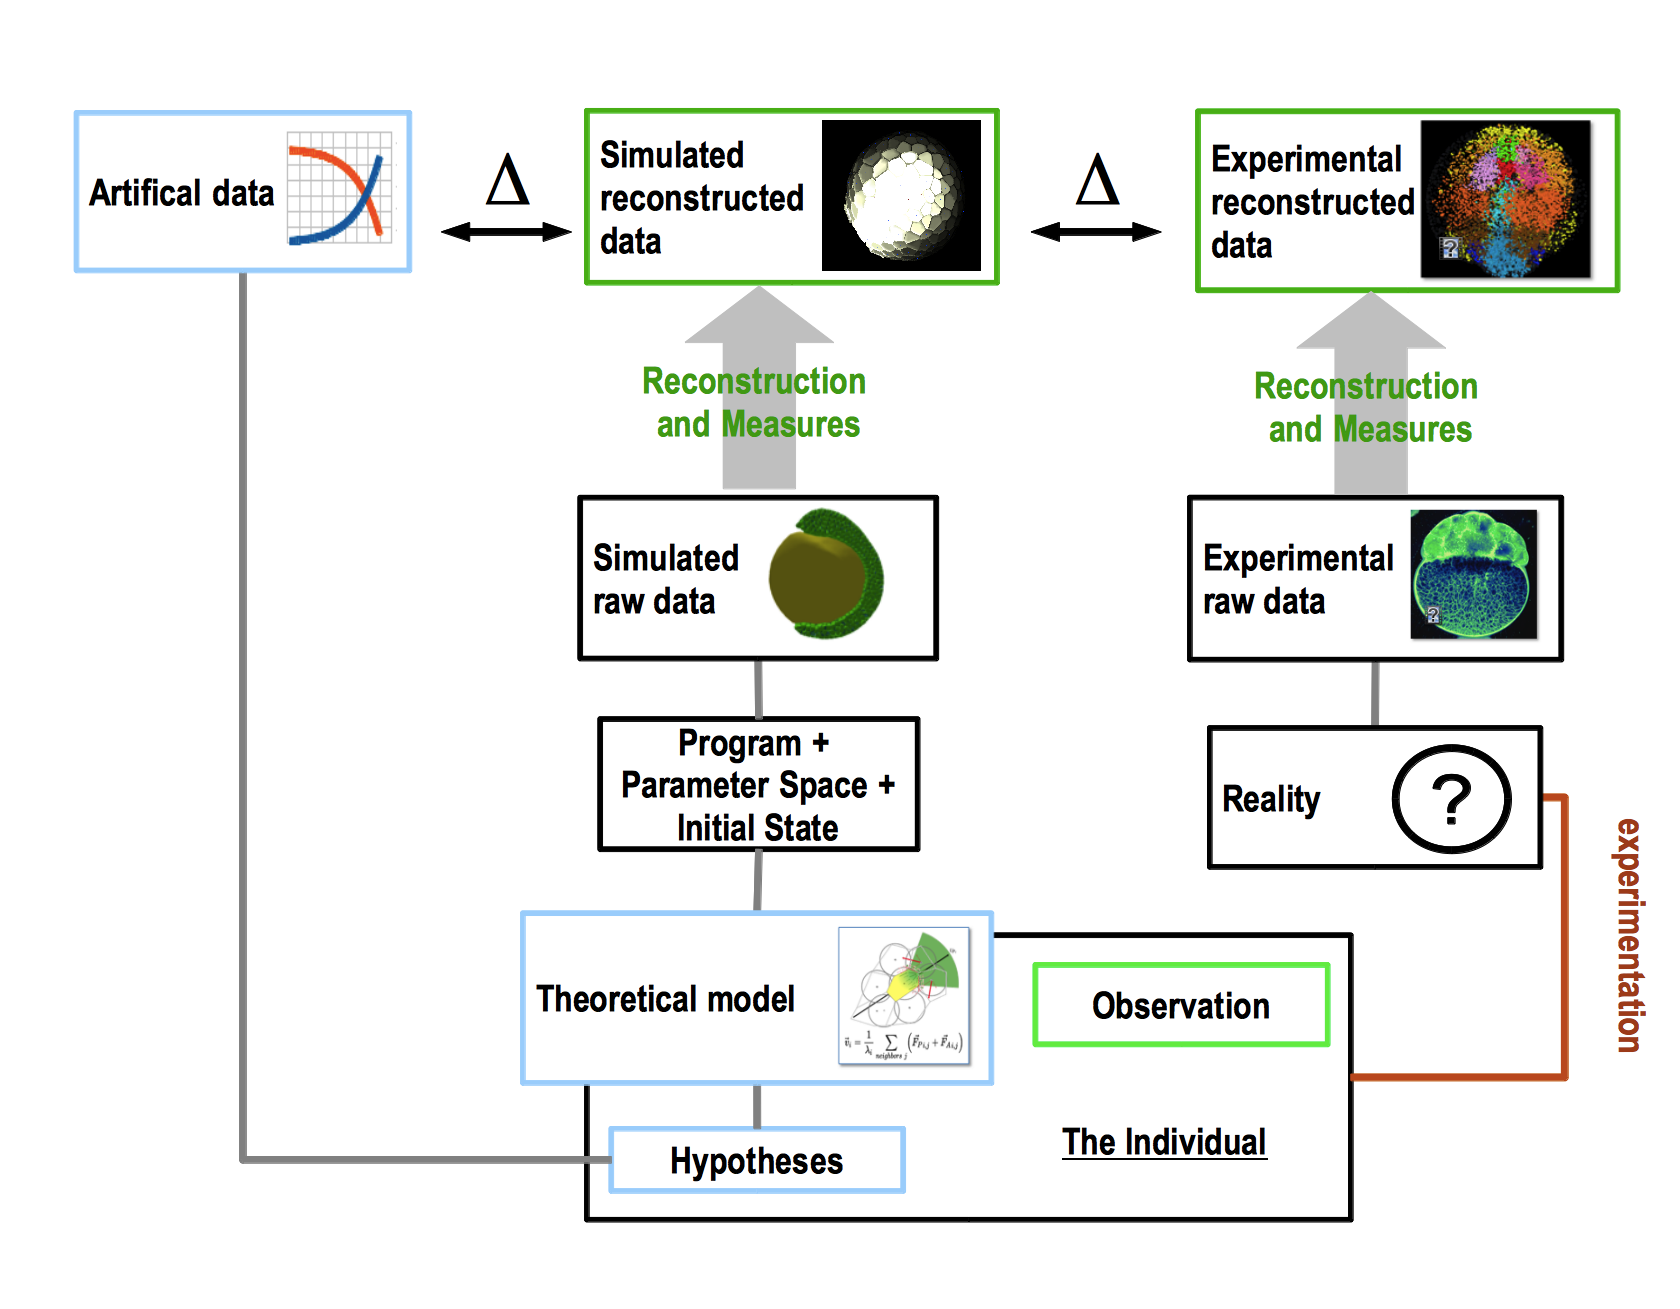
\includegraphics[width=0.95\textwidth]{../../images/experimental_science/experimental_science_cleaner.png}
\end{center}
\caption{\textbf{The chapter 8 involves all component of the methodological workflow introduced in Section 1.1.3.}}
\label{experimental_science_experimental_science_cleaner_chap8}
\end{figure}
%  ====================================================================== 


\subsection{Investigating the Yolk Biomechanical Properties}
%  ====================================================================== 


We assume that the early development of the embryo depends on \textit{viscoelastic properties} of the yolk. Using our simulation framework, our aim is to identify these properties by assessing their effect on later morphogenesis. In particular, we expect that yolk properties help maintain the integrity of the whole embryo, for example that the yolk should resist pressure exerted by the cells. At the same time, it should also undergo successive transformations by flattening at the sphere stage, and protruding at the doming stage. In addition, its active role in gastrulation is highly debated \cite{Behrndt:2012gy}. Several of these aspects will be investigated in the following sections. We show here that minimal viscoelastic properties are sufficient to account for some of the embryo's phenotypic features throughout cleavage and gastrulation.
%  ---------------------------------------------------------------------- 


\subsubsection{Hypotheses and Model}
%  ---------------------------------------------------------------------- 


Our model is based on state-of-the-art observations. The zebrafish zygote is a large cell filled with cytoplasm and lipid droplets. These two fluids start to segregate before the first divisions, then the cytoplasm is gradually sucked into the dividing cells (Fig. \ref{Case_0_Yolk_THG_thg}). A lipid bilayer membrane progressively separates the cells at the animal pole from the lipid droplets, forming an independent structure called the \textit{yolk cell}. After the $9^{th}$ division cycle, the marginal deep cells divide with one daugthter cell fusing with the yolk, forming a structure just beneath the cells called the \textit{yolk syncytial layer} (YSL). Another layer, the \textit{yolk cortical layer} (YCL), completely envelops the yolk (See below).
\begin{figure}
\begin{center}
\includegraphics[width=0.9\textwidth]{../../images/Cases_Studies/Case_0_Yolk/THG/thg.png}
\end{center}
\caption{\textbf{\textit{Third harmonic generation} (THG) imaging of the zebrafish embryo adapted from \cite{Olivier:2010jz}}. Snapshots from the movie \href{http://public.iscpif.fr/~delile/morphogenesis/manuscript/pragma/figure.html?name=Case_0_Yolk_1_THG_imaging_the_zebrafish_embryo_from_the_one_cell_stage}{.S.1} going from the one-cell stage to the 64-cell stage. Developmental timing (min) indicated top left. Scale bar (100 microns) indicated bottom left.}
\label{Case_0_Yolk_THG_thg}
\end{figure}

In this context, from the zygote stage, we make the approximation that the cells and the yolk are independent structures---but to capture their dynamical mechanical interactions, we model both of them in the same particle-based paradigm. Furthermore, we hypothesize that it is relevant to distinguish between an external "yolk membrane" (ym), which is composed of the YSL and YCL together, and the inner lipid droplets, or "yolk interior" (yi). Thus we use three types of particles: one for the cells (displayed in green in Fig. \ref{Case_0_Yolk_general_particles_yolk}) and two for the yolk: the membrane particles (in yellow) forming a 2D viscoelastic layer, and the interior particles (in red) representing the lipid droplets confined by the external layer. We expect the external membrane to keep its surface topology, whereas the internal structure can rearrange itself. This is a qualitative interpretation of imaging that provides plausible properties (\href{http://public.iscpif.fr/~delile/morphogenesis/manuscript/pragma/figure.html?name=Case_0_Yolk_1_THG_imaging_the_zebrafish_embryo_from_the_one_cell_stage}{.S.1}).
\begin{figure}
\begin{center}
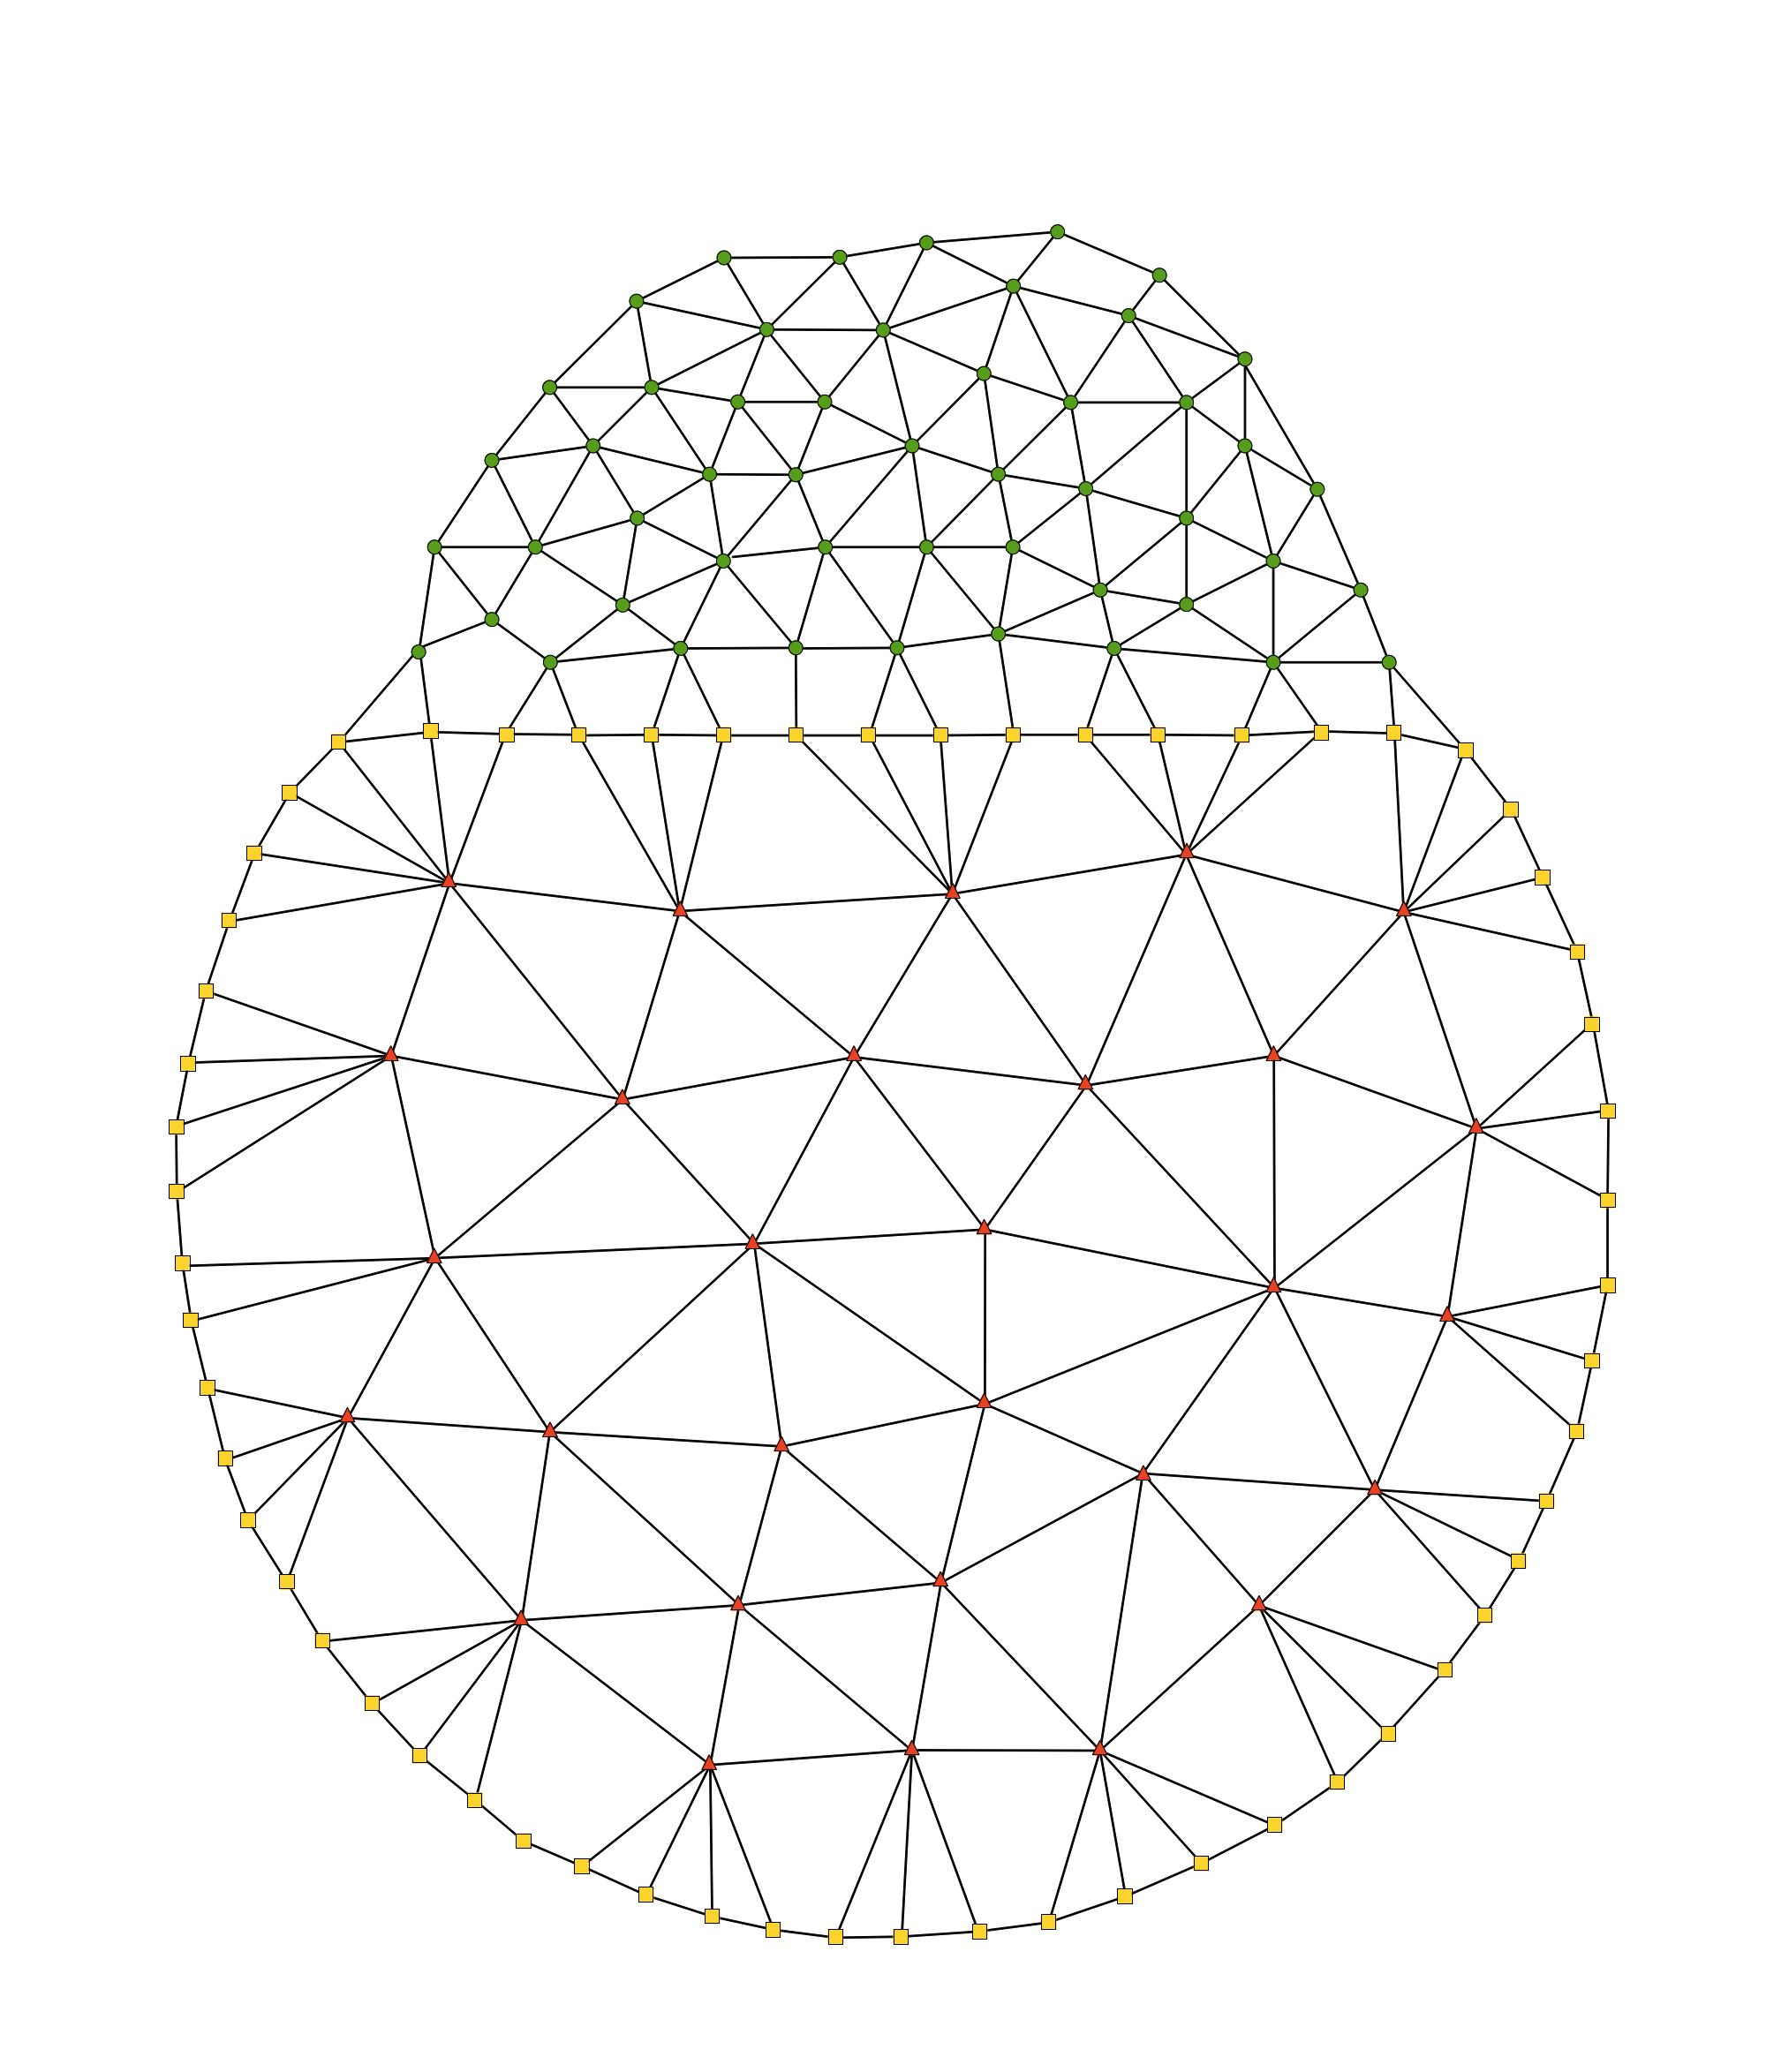
\includegraphics[width=0.6\textwidth]{../../images/Cases_Studies/Case_0_Yolk/general_particles_yolk.png}
\end{center}
\caption{\textbf{Abstract schema of the particle types in the modeled embryo.} Green particles represent the cells, yellow particles the external "yolk membrane" (ym), and red particles the inner lipid droplets or "yolk interior" (yi).}
\label{Case_0_Yolk_general_particles_yolk}
\end{figure}

\paragraph{The yolk membrane (ym)}
%  ++++++++++++++++++++++++++++++++++++++++++++++++++++++++++++++++++++++ 


In Fig. \ref{Case_0_Yolk_general_particles_yolk}, the yellow particles materialize the yolk membrane. Note that, whether we are talking of the YSL or the YCL, this "yolk membrane" is not only composed of a lipid bilayer but also a cytoskeleton that underlies it (acto-myosin network, micro-tubules, etc.). Here, the membrane topology is defined by a geodesic dome derived from an icosahedron, one of the five "Platonic solids", which remains invariant through time. An icosahedron's surface is composed of 20 identical equilateral triangles, 12 vertices and 30 edges. This topology is refined by subdividing each triangle into four new identical equilateral triangles. The new vertices are projected on the sphere. This process is repeated 4 times to approximate a spherical shape with 5120 triangles and 2562 vertices (Fig. \ref{Case_0_Yolk_blender_all_gl_zoom}). Although other Platonic solids could have been used without much difference, the icosahedron offers a better trade-off between stability (its elementary faces are triangles) and volume maximization (only the dodecahedron occupies a slightly larger volume, but its faces are pentagonal). In our geodesic dome, each vertex except the original 12 has 6 direct neighbors, the original vertices having only 5 direct neighbors. These direct neighbors are labeled "rank-1" neighbors. For each ym particle $i$, this neighborhood is denoted by $\mathcal{N}^{\mathrm{ym},1}_i$.

The forces exerted between ym particles are pure elastic forces. Each rank-1 neighborhood relationship is materialized by a linear spring, so that between two ym particles $(i,j)$, the force is simply:

$$\vec{F}^{\mathrm{ym}}_{ij} = -k_{\mathrm{ym}} (r_{ij} - r^{\mathrm{eq}}_{ij}) \vec{u}_{ij}$$

where $k_{\mathrm{ym}}$ is the stiffness constant controlling the ability to deform the neighborhood link under a given force applied to it (a higher $k_{\mathrm{ym}}$ creating a stiffer resistance), and $r^{\mathrm{eq}}_{ij}$ is the resting length of the neighborhood link (i.e. its length if no force is applied). Each ym-to-ym link has its own characteristic resting length. It is defined by the length of the link when the ideal geodesic dome is projected on a sphere whose volume is equal to the desired total yolk volume $V_{\mathrm{Y}}$, i.e. the radius is $R_{\mathrm{Y}} = (3V_{\mathrm{Y}}/4\pi)^{1/3}$. Concretely, the dozen 5-neighbor vertices have shorter resting lengths than all the other 6-neighbor vertices. Without this rescaling, the equilibrium shape would converge toward the original Platonic solid and not toward the sphere.

Since the ym neighborhood topology is invariant (ym particles do not "swarm", so the geodesic links remain the same), there is no plasticity in the yolk membrane alone. The original shape is recovered after local mechanical deformation (local pushing or pulling). Beyond a certain level of stress, however, the membrane mesh may get entangled and erratic behavior may occur. This is illustrated by an "abnormal" lip formed by the yolk membrane when ym particles are only interacting with their rank-1 neighbors (Fig. \ref{Case_0_Yolk_erratic_topology}A). We hypothesize that increasing the ym stiffness and the spatial range of particle interactions would prevent this undesirable feature. When constraining ym particles to rank-1 and rank-2 interactions, the blastoderm-yolk margin remains smooth (Fig. \ref{Case_0_Yolk_erratic_topology}B). Rank-2 neighbors of a yolk membrane particle are defined as the set of rank-1 neighbors plus their rank-1 neighbors (Fig. \ref{Case_0_Yolk_blender_all_gl_zoom}F). All the corresponding links are materialized by linear springs with the same stiffness coefficient $k_{\mathrm{ym}}$ and resting lengths $r^{\mathrm{eq}}$ defined by the same procedure as rank-1 neighbors. The rank-2 neighborhood set is denoted by $\mathcal{N}^{\mathrm{ym},2}_i$.
\begin{figure}
\begin{center}
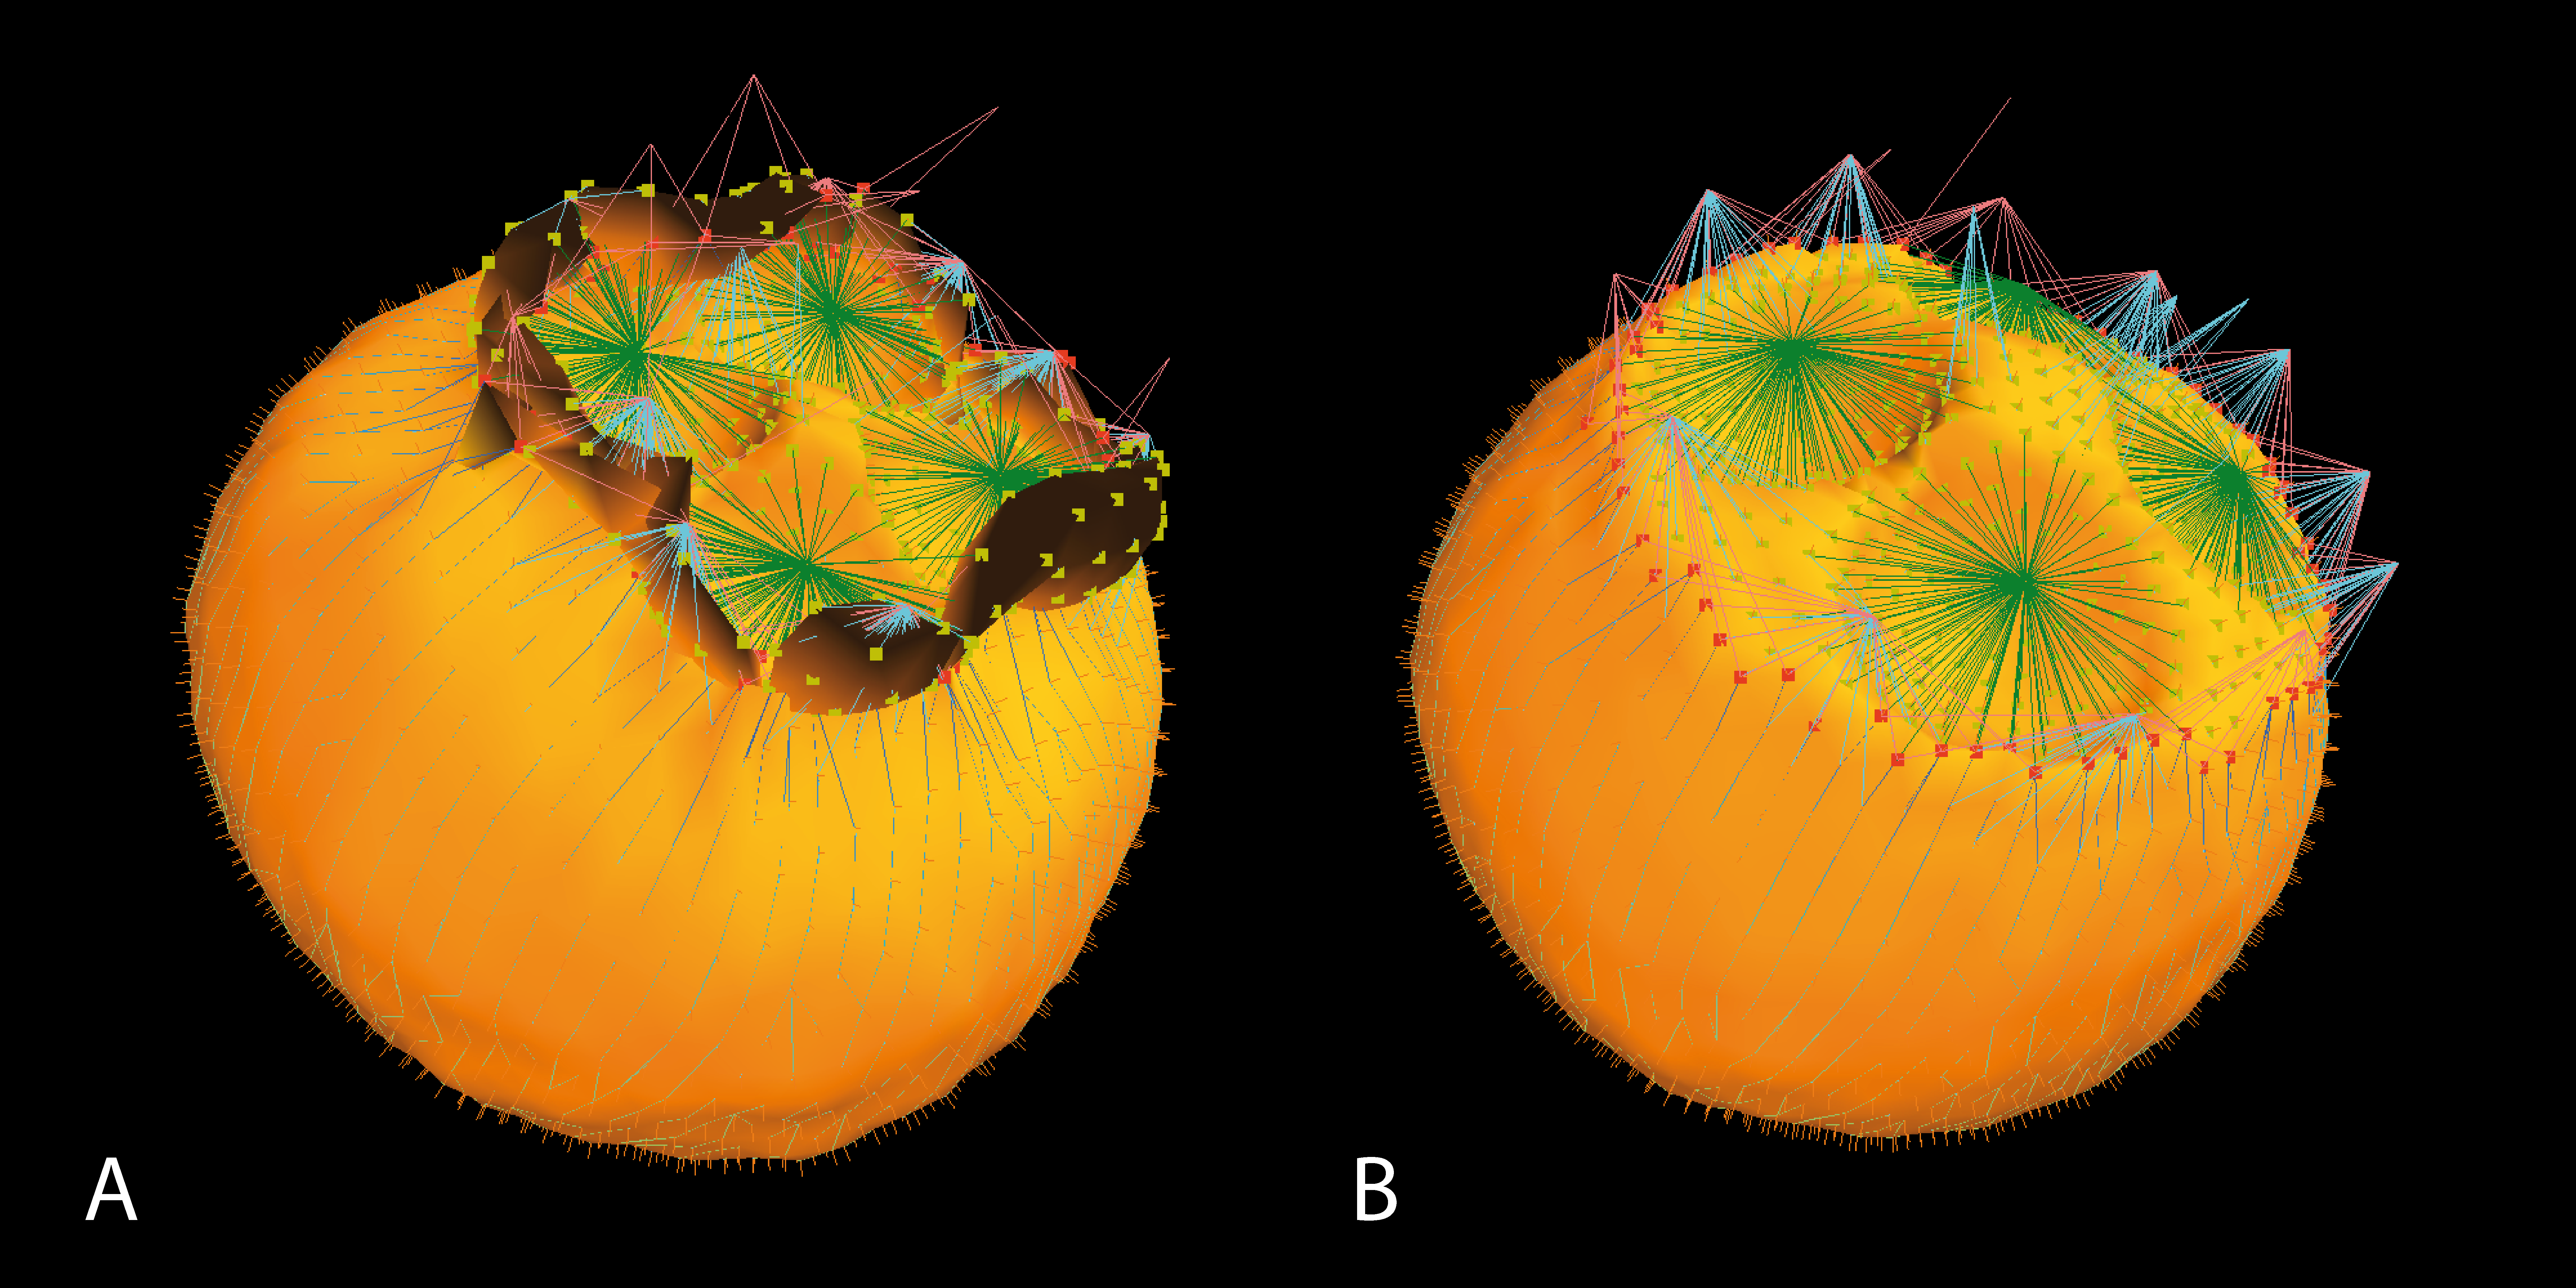
\includegraphics[width=0.9\textwidth]{../../images/Cases_Studies/Case_0_Yolk/erratic_topology.png}
\end{center}
\caption{\textbf{Yolk membrane behavior depending on its particles' topological interactions.} A: rank-1 interactions only. B: rank-1 + rank-2 interactions. }
\label{Case_0_Yolk_erratic_topology}
\end{figure}
\begin{figure}
\begin{center}
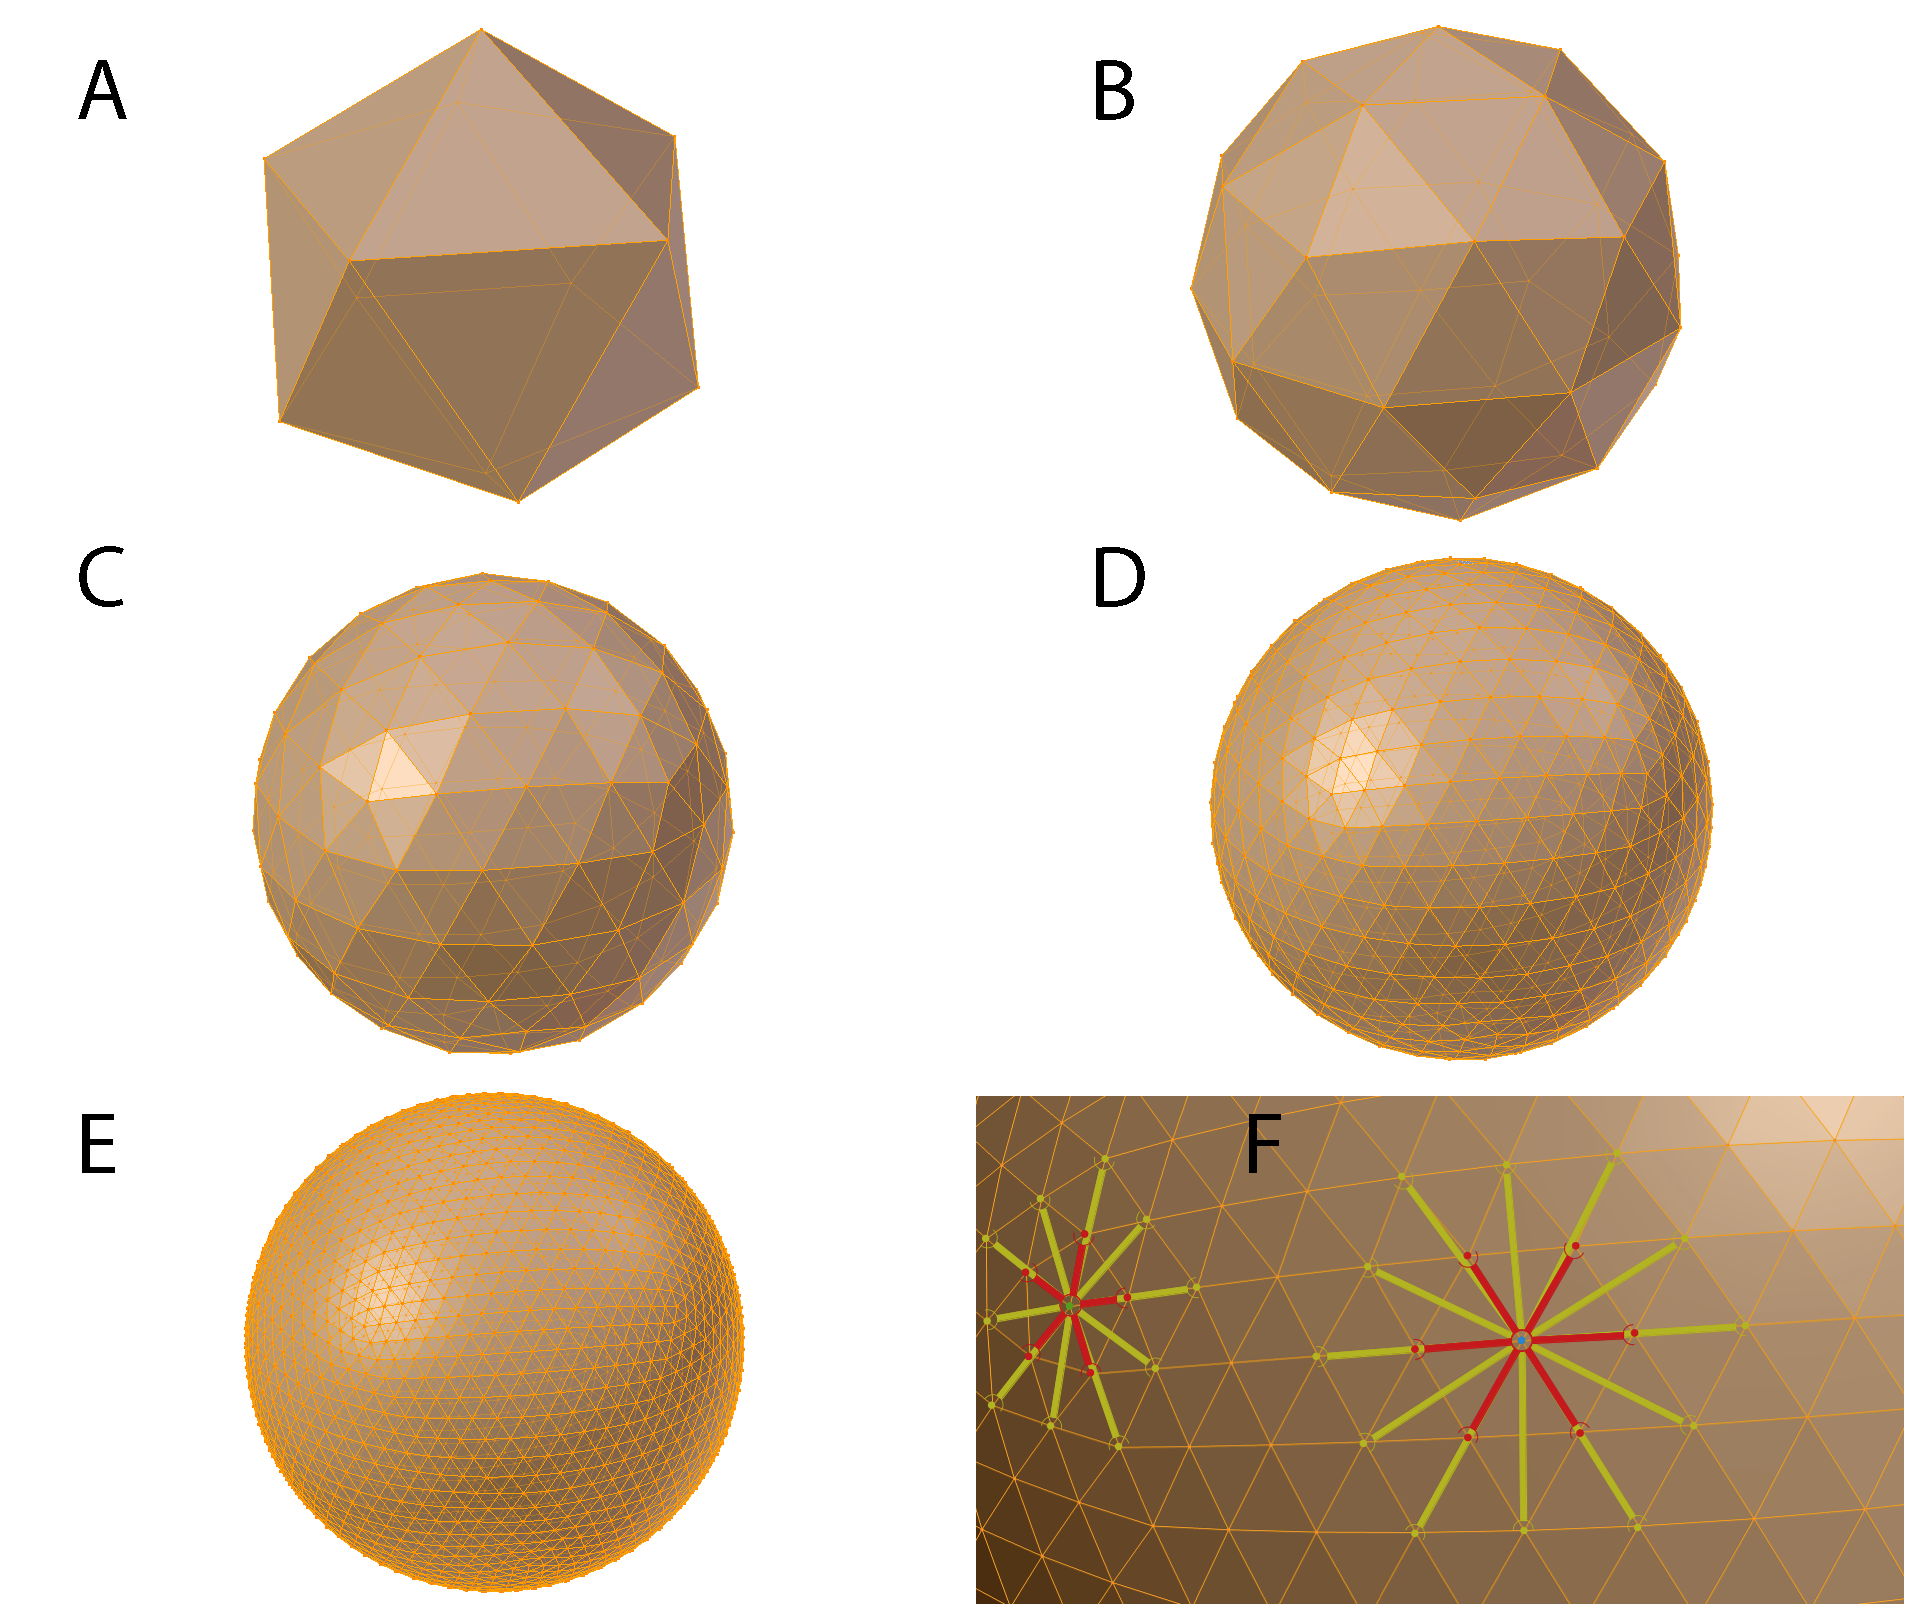
\includegraphics[width=0.9\textwidth]{../../images/Cases_Studies/Case_0_Yolk/blender/all_gl_zoom_letter.png}
\end{center}
\caption{\textbf{The structural topology of the yolk membrane is a geodesic dome.} A: Icosahedron. B,C,D,E: iterative subdivision of the original icosahedron to obtain the geodesic dome. F: the right vertex is a regular geodesic vertex and the left vertex is one of the 12 original icosahedral vertices. Rank-1 neighbors link in red, rank-2 neighbors link in yellow.}
\label{Case_0_Yolk_blender_all_gl_zoom}
\end{figure}

So far, we have idealized the yolk membrane as an "empty balloon". It must now be filled with a viscous fluid. In the real yolk, if the yolk membrane is damaged, inner material is expelled out of the membrane. This indicates that the inside pressure is higher than the outside. We hypothesized that this difference of pressure is due to the cortical tension exerted by the yolk membrane and introduce an additional parameter: $c_r \lt 1$, which is a dimensionless coefficient reducing the resting lengths within the yolk membrane. The above force equation then becomes:

$$ \vec{F}^{\mathrm{ym}}_{ij} = -k_{\mathrm{ym}} (r_{ij} - c_r r^{\mathrm{eq}}_{ij}).\vec{u}_{ij} $$

\paragraph{The yolk interior (yi)}
%  ++++++++++++++++++++++++++++++++++++++++++++++++++++++++++++++++++++++ 


The yolk membrane as modeled above has the ability to absorb and recover from tangential load but can hardly resist any load applied in a non-tangential manner. Inspired by the lipid droplets contours revealed by THG signals in Fig. \ref{Case_0_Yolk_THG_thg}, we fill the yolk interior (yi) with $N_{\mathrm{yi}}$ identical particles of volume $V_{\mathrm{yi}}$ and radius $R_{\mathrm{yi}}$ (red points in Fig. \ref{Case_0_Yolk_general_particles_yolk}). Practically, $N_{\mathrm{yi}} = 500$ particles were added in our simulation, which is less than the number of lipid droplets estimated from the 3D data, and represents a coarse-grained approximation. We assume that the ym particles' radius is equal to the yi particles' radius, so that the volume occupied by the $N_{\mathrm{yi}}$ particles is equivalent to the volume of a sphere minus the thickness of the ym layer, i.e. whose radius is $R_{\mathrm{Y}} - R_{\mathrm{ym}} = R_{\mathrm{Y}} - R_{\mathrm{yi}}$.

$$ N_{\mathrm{yi}} \frac{4}{3} \pi R_{\mathrm{yi}}^3 = \frac{4}{3} \pi (R_{\mathrm{Y}} - R_{\mathrm{yi}})^3 \;\;\Leftrightarrow\;\; R_{\mathrm{yi}} = \frac{R_{\mathrm{Y}}}{1 + \sqrt[3]{N_{\mathrm{yi}}}}$$

and with $R_{\mathrm{Y}} \gg R_{\mathrm{yi}}$, we get $R_{\mathrm{yi}} \approx R_{\mathrm{Y}} (N_{\mathrm{yi}})^{1/3}$. We apply the same rules as the ones described for cell-cell interactions in Chapter 3 to ym-yi and yi-yi pairs of particles. As in Section 3.2.2, the neighborhood of interactions is recalculated at every time step of the simulation, first through a metric criterion then by topological selection. This adaptive topology provides to the yolk a certain plasticity through passive rearrangement of the yi particles. Both ym-yi and yi-yi interaction forces have the same expression as the passive attraction/repulsion forces between deep cells particles (see Section 3.2.3):

$$\vec{F}^{\mathrm{y}}_{ij} = A_{ij}.\vec{F}^{\mathrm{y},\mathrm{lin}}_{ij} =  \begin{cases}  - w^{\mathrm{y}}_{\mathrm{rep}}(r_{ij}-r^{\mathrm{eq}}_{ij}) A_{ij}.\vec{u}_{ij} & \text{if }r_{ij} \lt r^{\mathrm{eq}}_{ij} \\  - w^{\mathrm{y}}_{\mathrm{adh}}(r_{ij}-r^{\mathrm{eq}}_{ij}) A_{ij}.\vec{u}_{ij} & \text{if }r_{ij} \geq r^{\mathrm{eq}}_{ij} \;\text{and }r_{ij} \lt r^{\mathrm{max}}_{ij} \\  \vec{0} & \text{if }r_{ij} \geq r^{\mathrm{max}}_{ij}  \end{cases}$$

where "y" stands for either ym-yi or yi-yi types of interactions, and $w^{\mathrm{y}}_{\mathrm{adh}}$ and $w^{\mathrm{y}}_{\mathrm{rep}}$ are unique yolk-specific stiffness coefficients common to both types.

\paragraph{Parameter space for the biomechanical properties of the yolk}
%  ++++++++++++++++++++++++++++++++++++++++++++++++++++++++++++++++++++++ 


In summary, putting together the ym and yi force expressions above, the equation of motion of the $N_{\mathrm{ym}}$ particles of the yolk membrane reads:

$$\vec{v}^{\mathrm{ym}}_{i} =  \frac{1}{\lambda_{0} {R_{\mathrm{ym}}}^2} \left( \sum_{j \in \mathcal{N}^{\mathrm{ym},2}_i} -k_{\mathrm{ym}} (r_{ij} - c_r r^{\mathrm{eq}}_{ij}).\vec{u}_{ij} + \sum_{j \in \mathcal{N}^t_i} \vec{F}^{\mathrm{y}}_{ij} \right)$$

and the equation of motion for the $N_{\mathrm{yi}}$ particles of the yolk interior is:

$$\vec{v}_{i} =  \frac{1}{\lambda_{0} {R_{\mathrm{yi}}}^2} \sum_{j \in \mathcal{N}^t_i} \left( \vec{F}^{\mathrm{y}}_{ij} \right)$$

where neighborhood $\mathcal{N}^{\mathrm{ym},2}_i$ contains only ym-type particles and $\mathcal{N}^t_i$ contains both ym and yi types. This system of equations is controlled by the following parameters: $\lambda_0$, $w^{\mathrm{y}}_{\mathrm{adh}}$, $w^{\mathrm{y}}_{\mathrm{rep}}$, $k_{\mathrm{ym}}$, $c_r$, the simulation time step $\Delta\!t_s$ and a number of other background parameters such as $R_{\mathrm{ym}}$, $R_{\mathrm{yi}}$, $a$, and $c^{\mathrm{max}}$ (in the expression of $A_{ij}$), which were a priori fixed or pre-calibrated when designing the simulation. The simulation, parameter space exploration and validation process described in the next subsection will allow us to estimate realistic values for the following ratios:
\begin{itemize}
	\item $\overline{w}^{\mathrm{y}}_{\mathrm{adh}} = w^{\mathrm{y}}_{\mathrm{adh}}/\lambda_0$
	\item $\overline{w}^{\mathrm{y}}_{\mathrm{rep}} = w^{\mathrm{y}}_{\mathrm{rep}}/\lambda_0$
	\item $\overline{k}_{\mathrm{ym}} = k_{\mathrm{ym}}/\lambda_0$
\end{itemize}

the last two undetermined or "free" parameters being the yolk membrane surface scaling parameter $c_r$ and the simulation time step $\Delta\!t_s$.
%  ---------------------------------------------------------------------- 


\subsubsection{Simulation, Parameter Space and Validation }
%  ---------------------------------------------------------------------- 


We expect the yolk to exhibit a specific behavior of \textit{deformation} under external stress followed by a behavior of \textit{resilience} through recovery. In order to assess the relevance of these properties, we designed an experimental protocol applied to both live specimens and simulated ones. As in most of the case studies explained in this Chapter 8, confronting measurements in both cases is our strategy to explore the parameter space, with the goals of:
\begin{itemize}
	\item qualitatively discussing the fitness landscape, and
	\item finding optimal parameters.
\end{itemize}

\paragraph{Experimental protocol: live specimen}
%  ++++++++++++++++++++++++++++++++++++++++++++++++++++++++++++++++++++++ 


A spherical 1-cell-stage embryo lying on its side in an agarose mold, a glass bead is pressed on the lateral side of the embryo for a period of time $\Delta\!T$, starting at $t_0$. The force is applied along an axis parallel to the agarose surface and, on the opposite side, the embryo is blocked by an agarose wall. Pressure is applied to the bead until it enters into the yolk by approximatively 40% of the yolk diameter. At $t_1 = t_0 + \Delta\!T$, the bead is removed and the yolk progressively recovers its initial shape. The operation is recorded with a 3CCD camera (Hitachi HV-D20) on a Leica MZ16F stereo microscope (Movie \href{http://public.iscpif.fr/~delile/morphogenesis/manuscript/pragma/figure.html?name=121120_121120_raw_lateral_embryo1}{.8.1}).


Qualitatively, the yolk is deformable with the yolk membrane surrounding the bead in a crater-like structure somewhat larger than the bead diameter. After removing the bead, the yolk quickly recovers its shape. The following measurements allow us to quantify this process. We measured every time interval $\Delta\!t_{\mathrm{y}} =$ 0.8 second the normalized length of the yolk along the compression axis, defined as the ratio of the deformed embryo's diameter $L$ over the relaxed embryo's diameter $L_{\mathrm{rel}}$ before compression.
\begin{figure}
\begin{center}
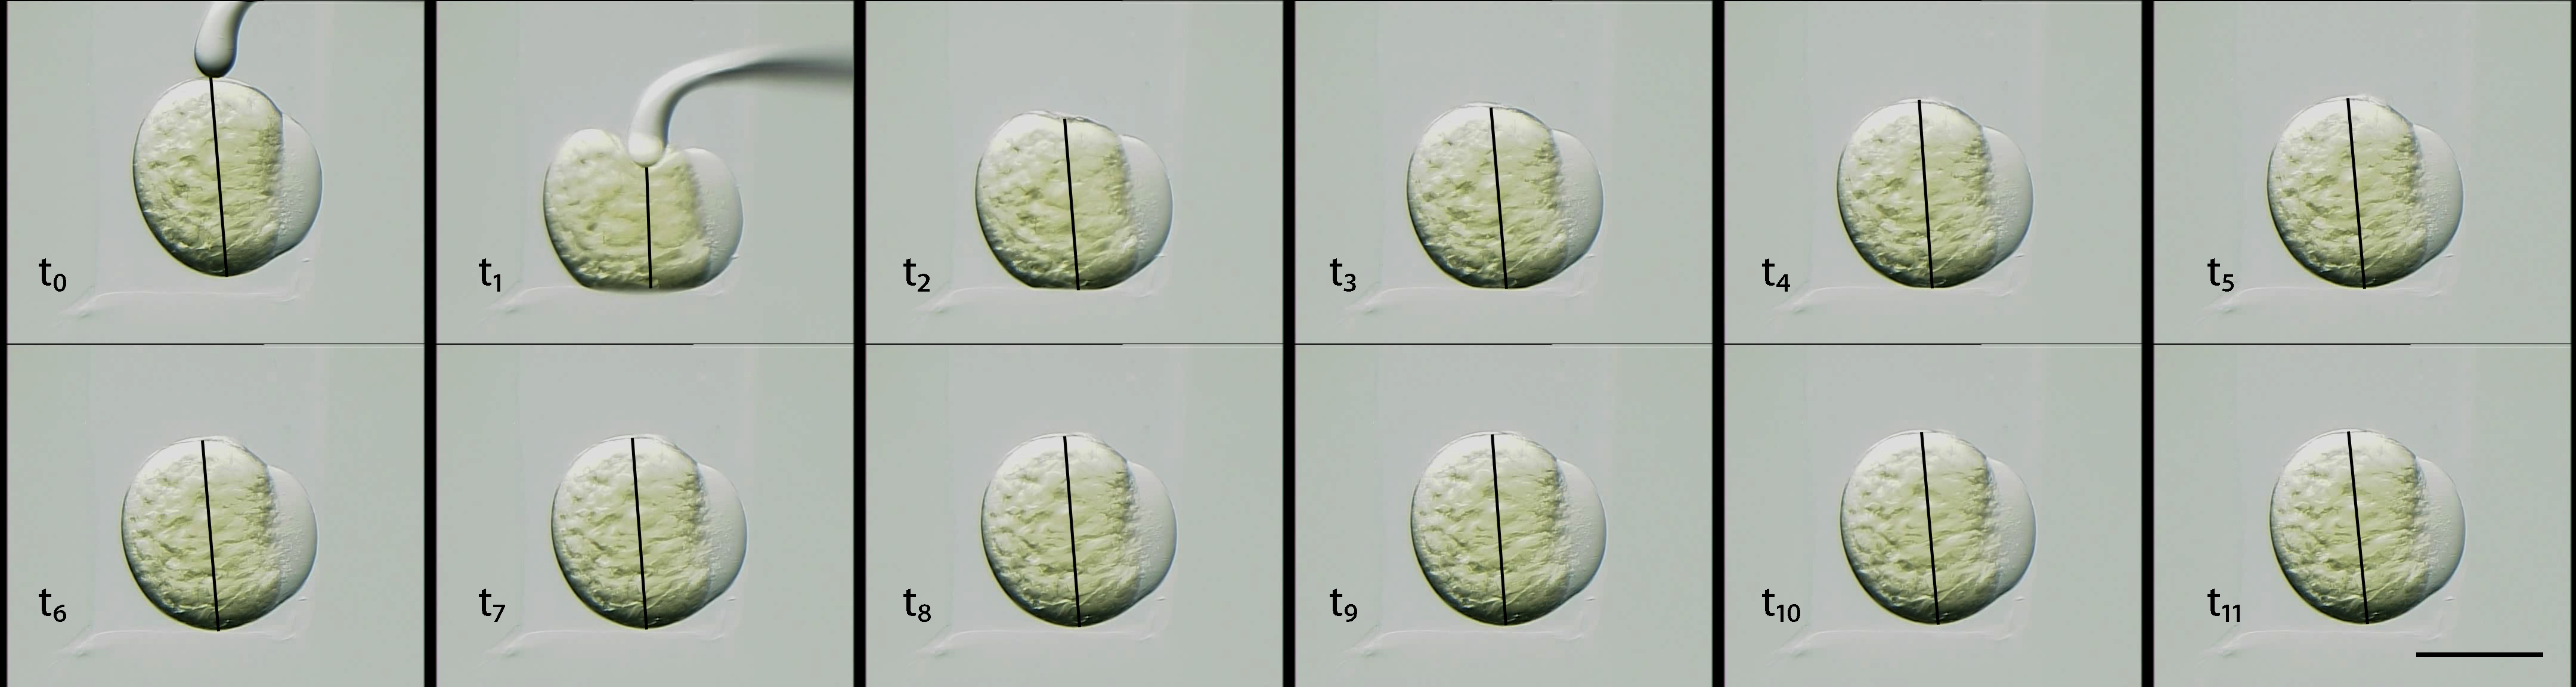
\includegraphics[width=0.95\textwidth]{../../images/Cases_Studies/Case_0_Yolk/121120/121120_raw_embryo1_m.png}
\end{center}
\caption{\textbf{Experimental deformation of the egg yolk.} 1-cell stage, lateral view, animal pole to the right. $t_0$: Onset of the deformation. $t_1$: Maximum deformation. Measurement is realized every 0.8 second. We measure the distance $L$ between the area pointed by the tip of the bead and the opposite side (black line). Scalebar 500 microns. }
\label{121120_121120_raw_embryo1_m}
\end{figure}
\begin{figure}
\begin{center}
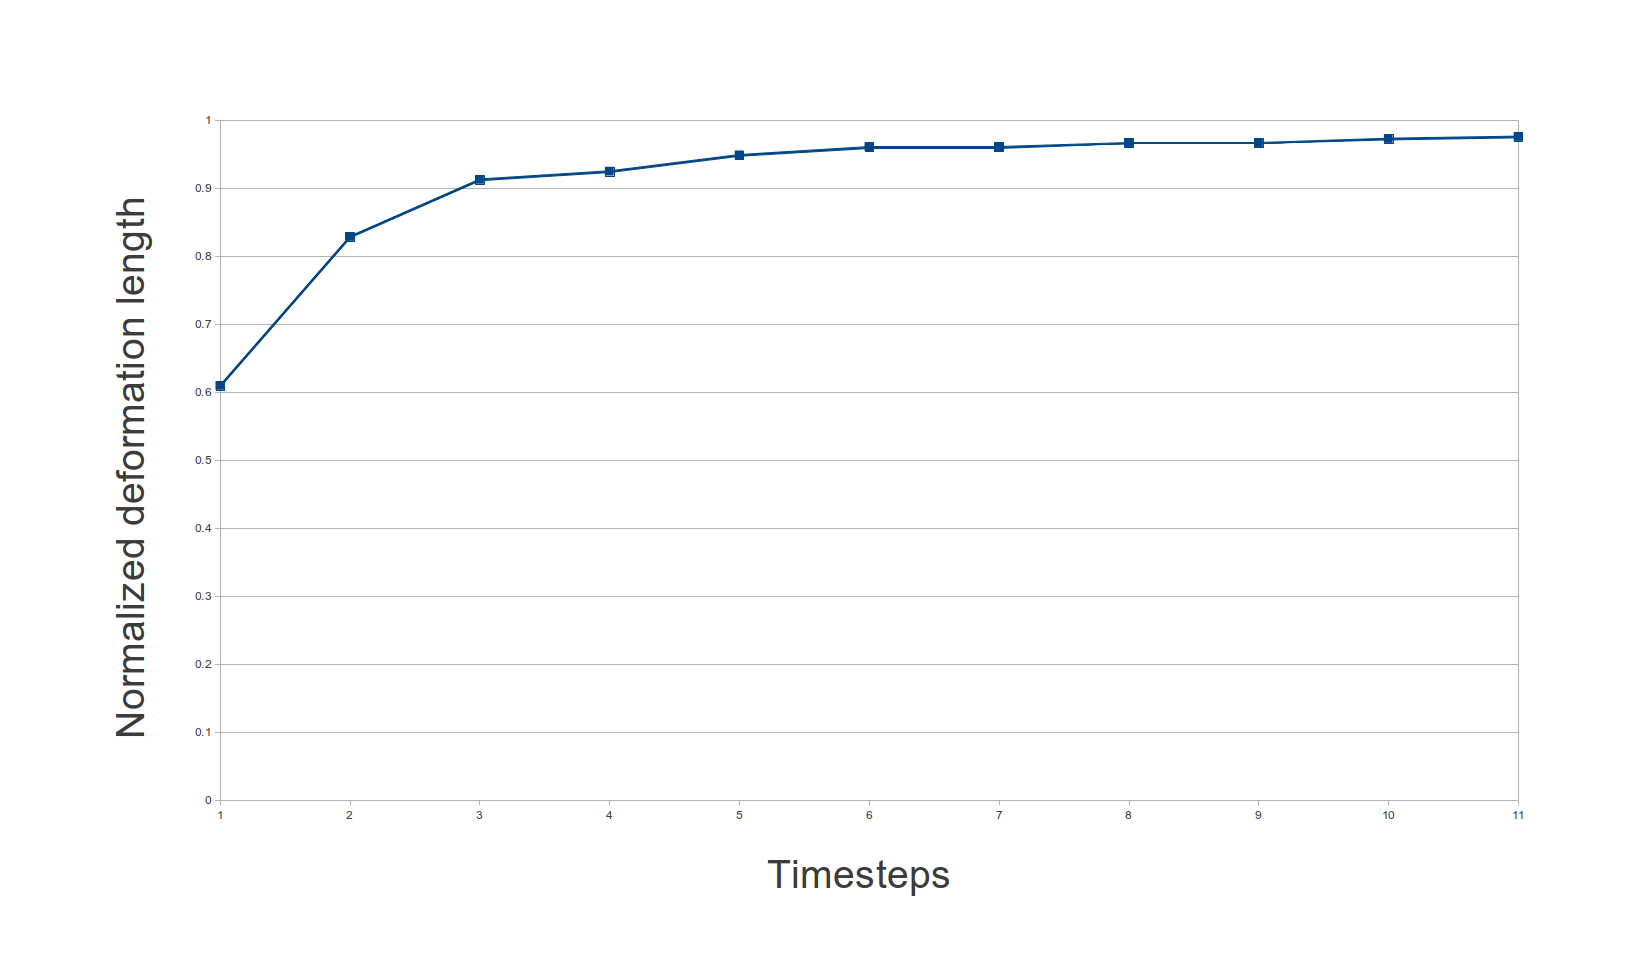
\includegraphics[width=0.8\textwidth]{../../images/Cases_Studies/Case_0_Yolk/plot_normalized_def.png}
\end{center}
\caption{\textbf{Plot of the normalized deformation length as a function of time.} The shape recovery is asymptotic toward the normalized length at $t_0$. Full recovery is nearly achieved by 8 seconds.}
\label{Case_0_Yolk_plot_normalized}
\end{figure}

\paragraph{Experimental protocol: simulation}
%  ++++++++++++++++++++++++++++++++++++++++++++++++++++++++++++++++++++++ 


The simulated experimental protocol mimics the live one described above. The algorithmic implementation of the model integrates an artificial spherical bead which is forced to move toward the center of the yolk. Yolk particles, whose original positions are now occupied by the bead, are displaced by being projected on the bead's surface. Similarly to the experimental live protocol, we specify the force necessary to induce the particles' motion but impose their displacement. The ball is removed when it has sunk to a depth equal to 40% of the initial yolk diameter.
\begin{figure}
\begin{center}
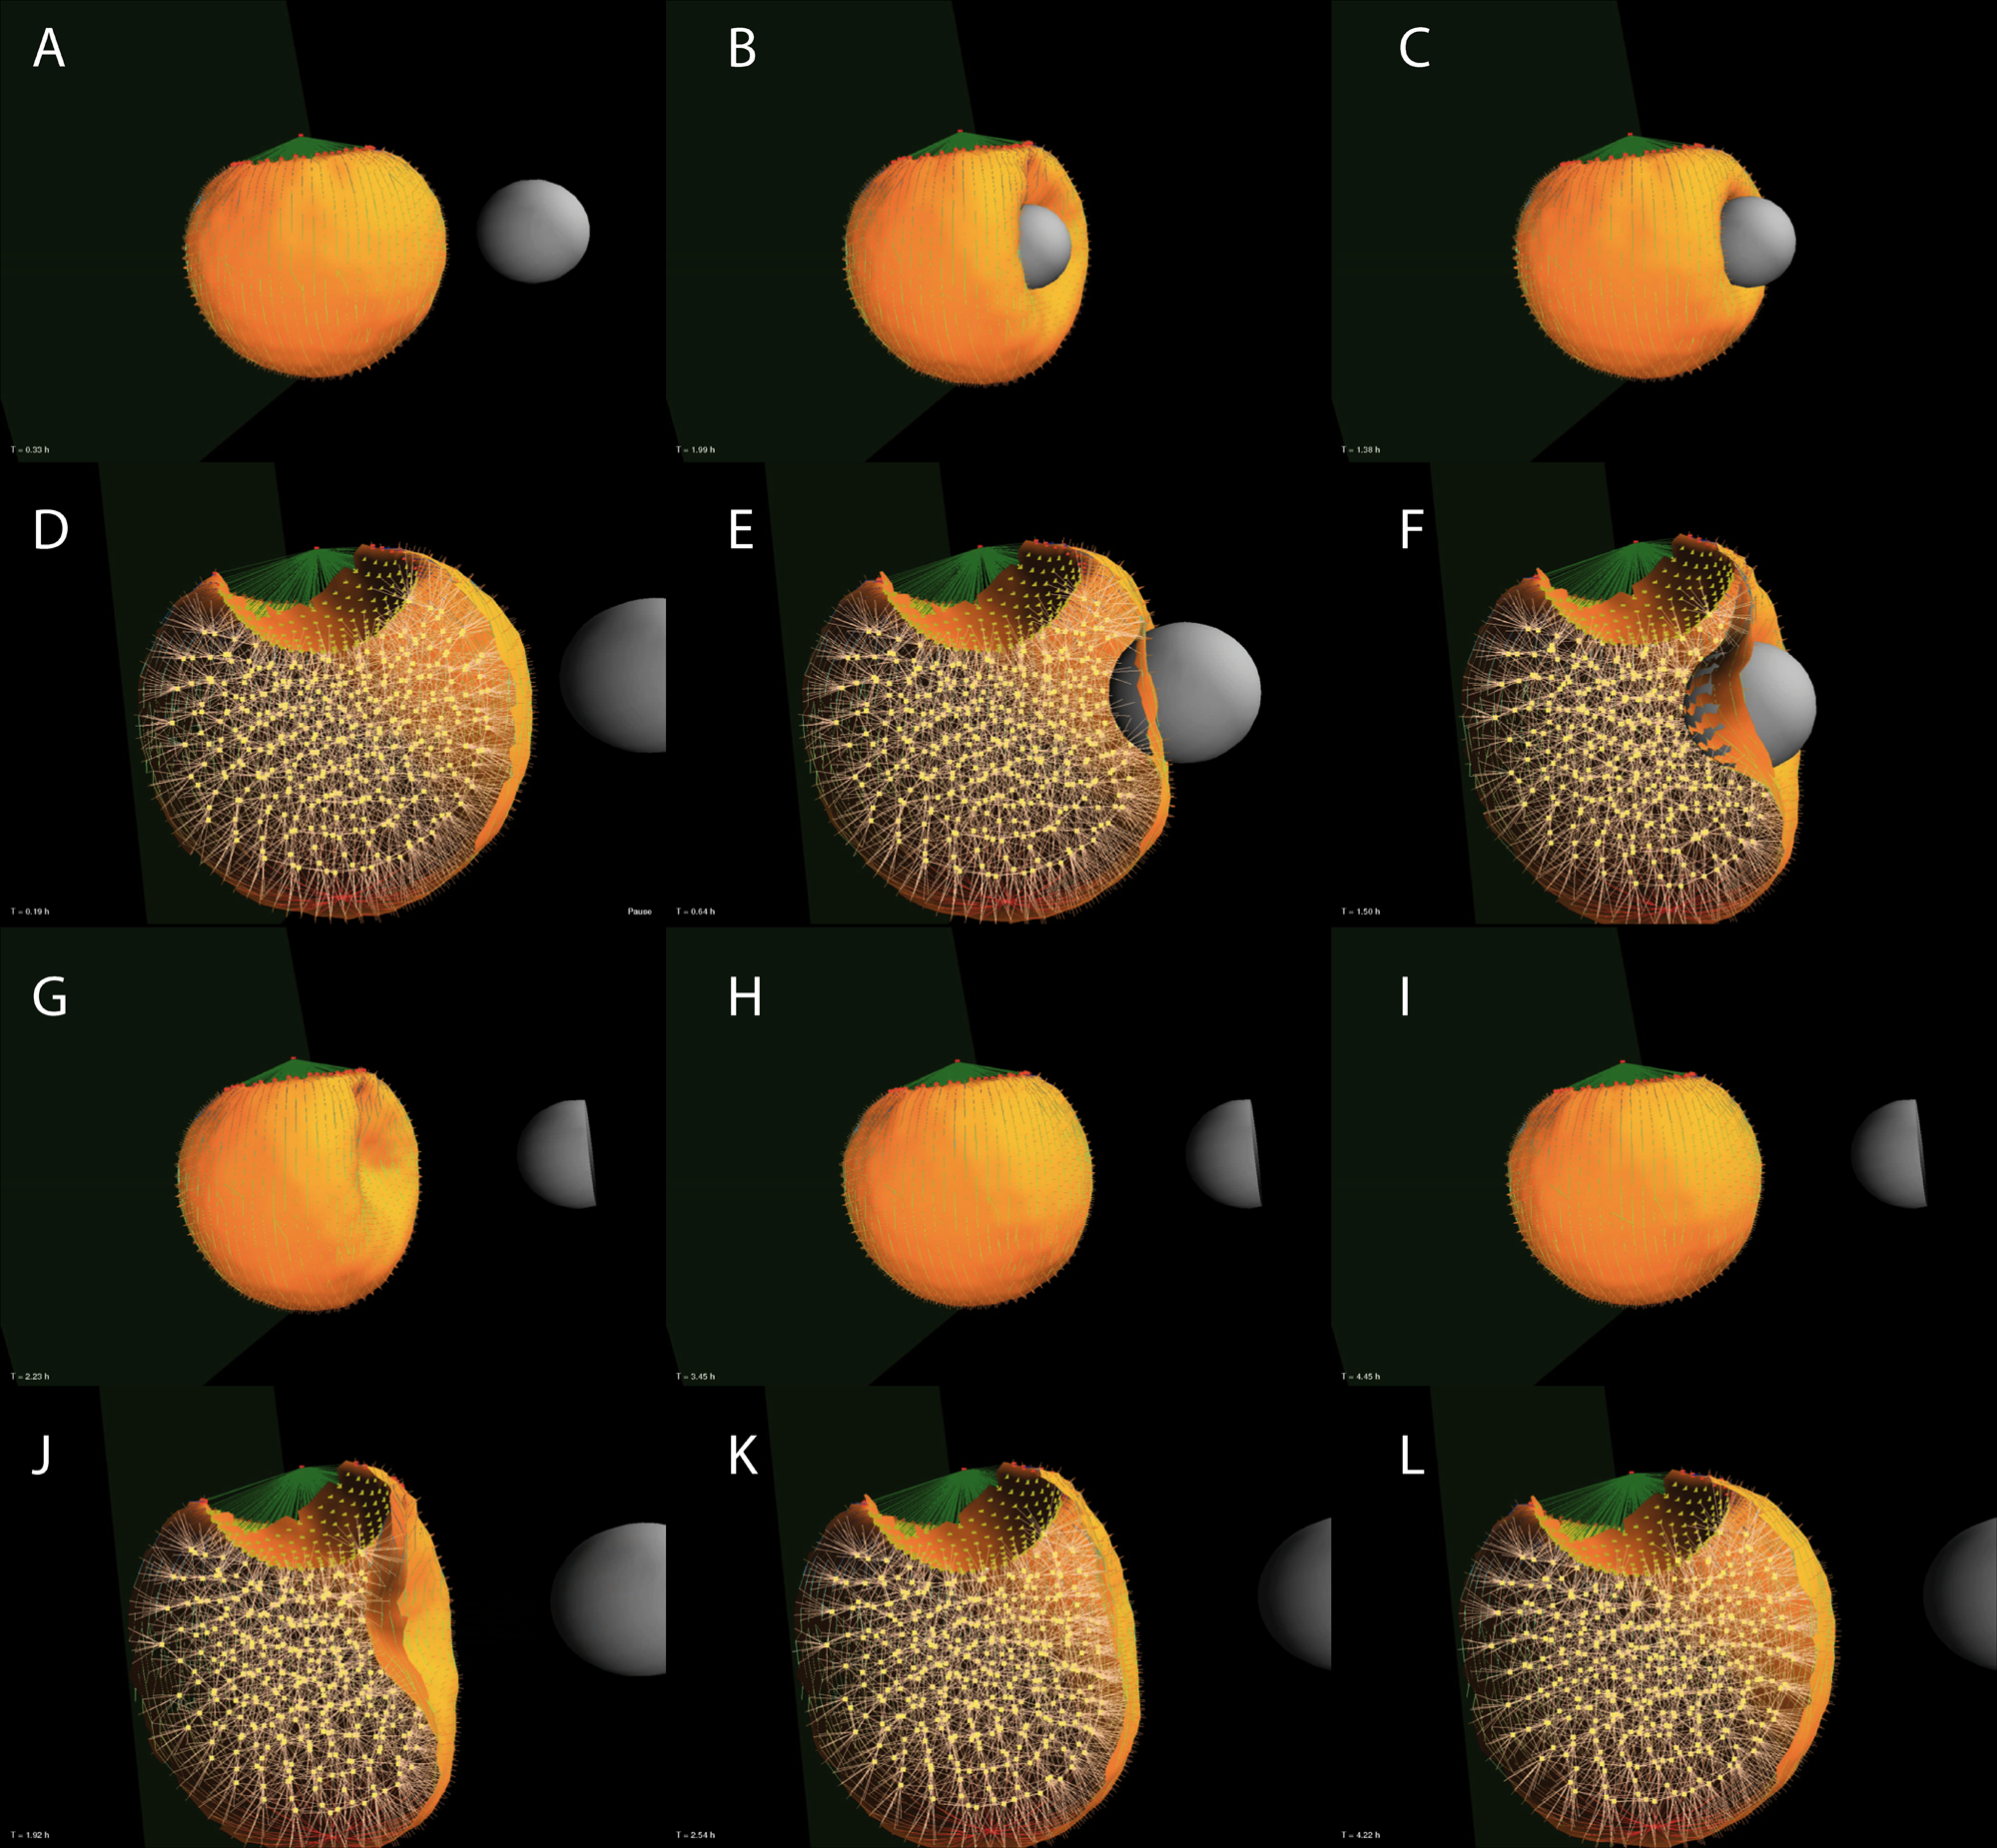
\includegraphics[width=0.7\textwidth]{../../images/Cases_Studies/Case_0_Yolk/simulation_example2.png}
\end{center}
\caption{\textbf{Snapshots of the simulated deformation and recovery.} First and third rows: entire yolk from an external point of view. Second and fourth rows: another yolk sliced to reveal the yolk interior particles. A,B,C,D,E,F: compression phase. G,H,I,J,K,L: relaxation phase.  Note that these simulated experiments have been realized by manually operating the spherical bead, whereas in the study the manipulation is automated. Original movies are available in Figs. \href{http://public.iscpif.fr/~delile/morphogenesis/manuscript/pragma/figure.html?name=Case_0_Yolk_yolk_external}{.S.3}\href{http://public.iscpif.fr/~delile/morphogenesis/manuscript/pragma/figure.html?name=Case_0_Yolk_yolk_relaxation_cut}{.S.4}}
\label{Case_0_Yolk_simulation_example}
\end{figure}

\paragraph{Fitness function}
%  ++++++++++++++++++++++++++++++++++++++++++++++++++++++++++++++++++++++ 


We define a fitness function $F_{\mathrm{Y,rel}}$ which allows us to confront the simulations and the measurements: it is an integral of the evolution (here, a discrete sum over time) of the absolute difference between the live and the simulated normalized length, starting at time $t_1$ when the pressure is removed, and ending at $t_n = t_1 + (n-1)\,\Delta\!t_{\mathrm{y}}$ with typically $n=10$. Denoting by $L^{\mathrm{s}}(t)$ and $L^{\mathrm{v}}(t)$ the deformed yolk diameters of the simulated and the live ("in vitro") specimens measured at time step $t$, the equation of the fitness function reads:

$$ F_{\mathrm{Y,rel}} = \sum_{t=t_1}^{t_n} \;\;\left | \frac{L^{\mathrm{s}}(t)}{L^{\mathrm{s}}_{\mathrm{rel}}} - \frac{L^{\mathrm{v}}(t)}{L^{\mathrm{v}}_{\mathrm{rel}}} \right | $$

where $L^{\mathrm{s}}_{\mathrm{rel}}$ and $L^{\mathrm{v}}_{\mathrm{rel}}$ are the initial uncompressed yolk diameters. Note that the lower the fitness values, the better the match.

\paragraph{Fitness landscape}
%  ++++++++++++++++++++++++++++++++++++++++++++++++++++++++++++++++++++++ 


We explore the parameter space of the simulation to find the best match with the measurements. This space is 4-dimensional, comprising $\overline{w}^{\mathrm{y}}_{\mathrm{adh}}$, $\overline{w}^{\mathrm{y}}_{\mathrm{rep}}$, $\overline{k}_{\mathrm{my}}$, and $c_r$, and was regularly sampled over the following ranges with the following numbers of values ("cardinalities"):
\begin{figure}
\begin{center}
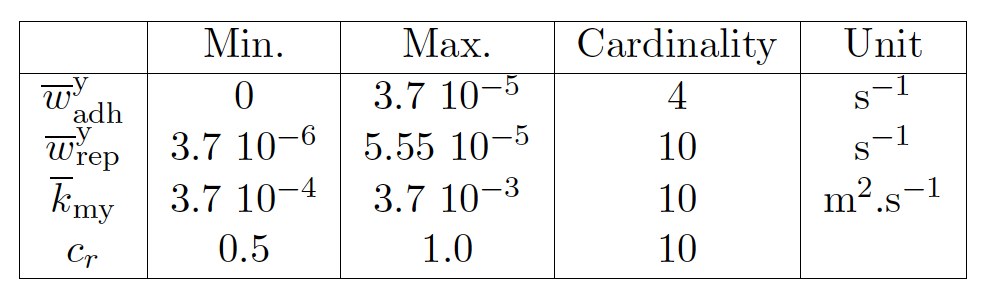
\includegraphics[width=0.5\textwidth]{../../images/Cases_Studies/Case_0_Yolk/parameter_space_table/parameter_space_table.png}
\end{center}
\caption{\textbf{Ranges, cardinalities and units of the four parameters explored in this study.}}
\label{parameter_space_table_parameter_space_table}
\end{figure}

For each "realization", i.e. simulation under a particular set of parameters, the fitness is evaluated. The simulation time step $\Delta\!t_s$ has been calibrated to match the slope of the relaxation curve obtained in the live experiment (Fig. \ref{Case_0_Yolk_all_curves_plot_fitness_ok}) and its calibrated value is here $\Delta\!t_s =$ 6.66667 milliseconds. This means that the yolk measurement time step $\Delta\!t_{\mathrm{y}}$ of 0.8 seconds is equivalent to 120 simulated time steps.
\begin{figure}
\begin{center}
\includegraphics[width=0.8\textwidth]{../../images/Cases_Studies/Case_0_Yolk/all_curves_plot_fitness_ok.png}
\end{center}
\caption{\textbf{Plots of the simulated normalized deformation length as a function of time.} The red thick curve represents the experimental live measurement. The simulated measurements are colored according to their fitness value (from red for the best fitness $F = 0.1609$ to blue for the worst $F = 7.1449$). In ordinate, the normalized length of the yolk diameter is plotted. In abscissa, the time from the moment the bead is pulled away from the yolk surface.}
\label{Case_0_Yolk_all_curves_plot_fitness_ok}
\end{figure}

This plot indicates that the simulated phenotype leads to a relaxation profile similar to the profile provided by the live experiment. However, another representation was needed to visualize the fitness pattern in the 4D parameter space. We developed an interface displaying the fitness as a 3D cube and selecting the fourth dimension manually (Fig. \ref{4D_fusion_vertical}).
\begin{figure}
\begin{center}
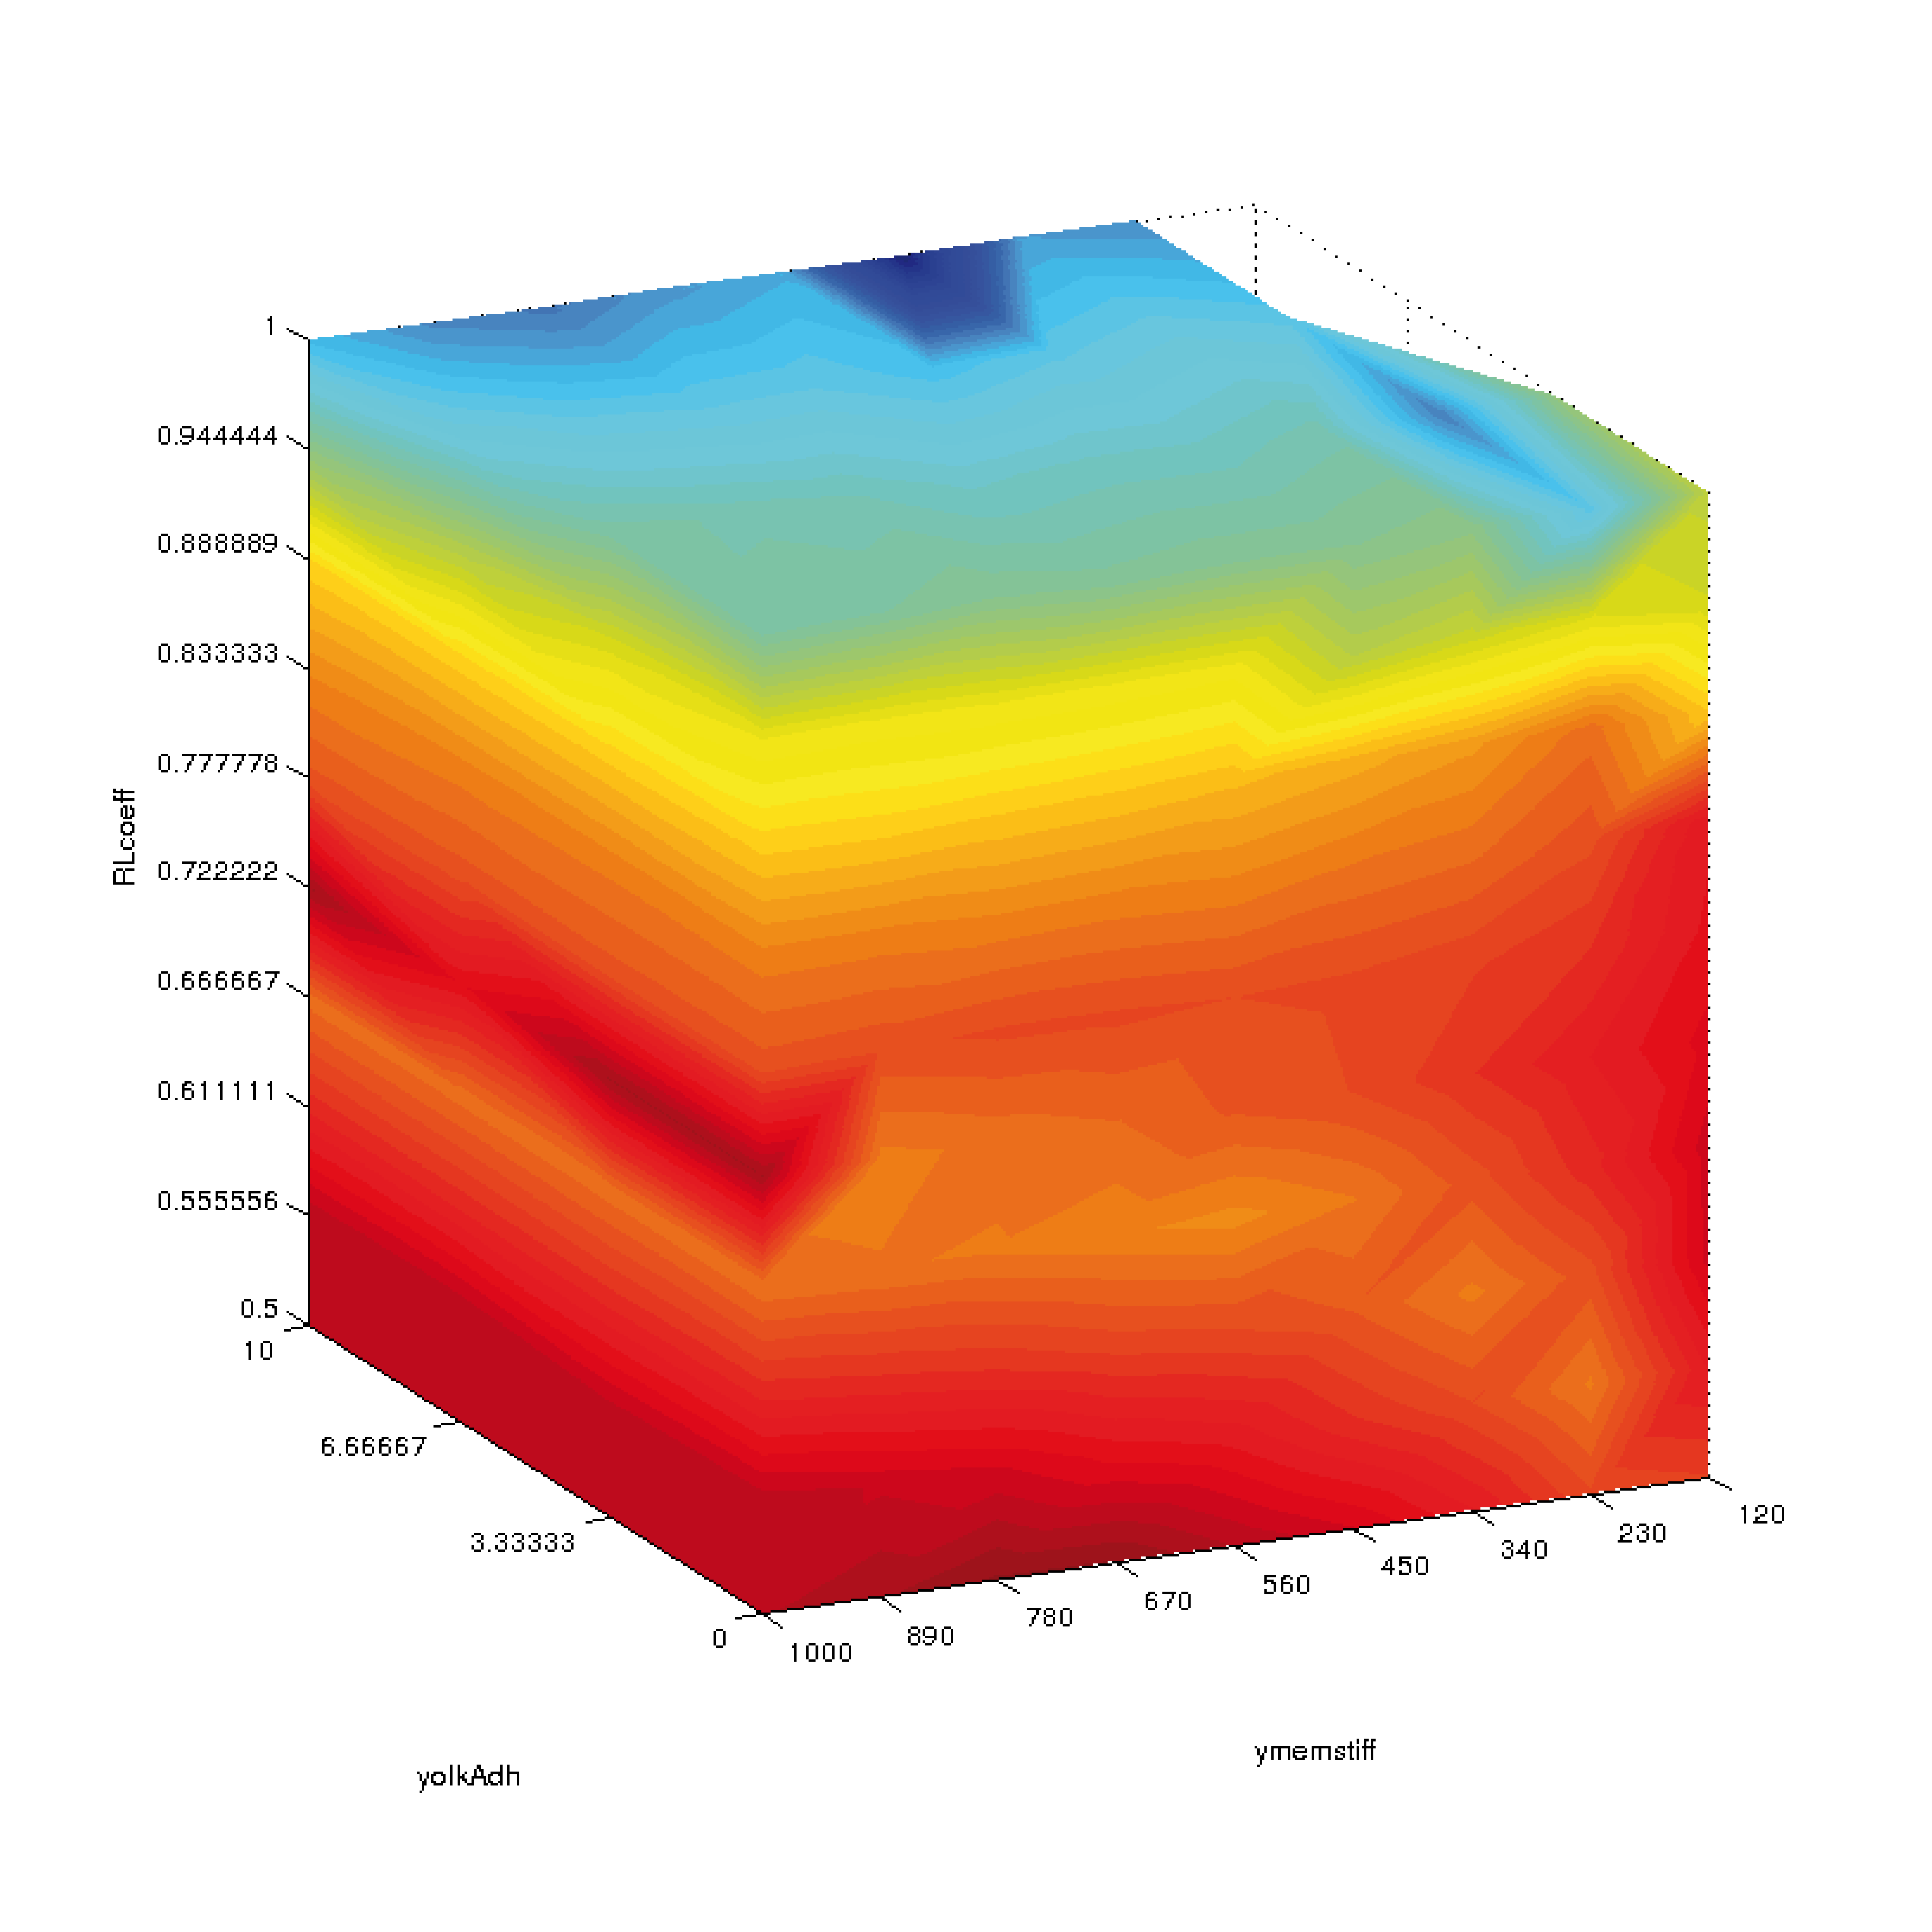
\includegraphics[width=0.8\textwidth]{../../images/Cases_Studies/Case_0_Yolk/4D/single_3D_plot.png}
\end{center}
\caption{\textbf{An example of 3D plot of the fitness landscape in parameter space.} This figure aims at presenting the coordinate system used in Fig. \ref{4D_fusion_vertical}. Here, the repulsion coefficient $\overline{w}^{\mathrm{y}}_{\mathrm{rep}}$ of the force exerted between yolk interior particles has a fixed value $3.7$ $10^{-6}$. The vertical axis is the coefficient $c_r$, which determines the equilibrium surface of the yolk membrane. The depth axis is the adhesion coefficient, $\overline{w}^{\mathrm{y}}_{\mathrm{adh}}$ which modulates the cohesion of the yolk interior particles. The width axis is the yolk membrane stiffness coefficient $\overline{k}_{\mathrm{ym}}$. It should be noted that the values plotted on the depth (resp. width) axis actually correspond to $w^{\mathrm{y}}_{\mathrm{adh}}$ (resp. $ k_{\mathrm{ym}}$) and should be divided by $\lambda_0$ to match the values of the table presented in Fig. \ref{parameter_space_table_parameter_space_table}.  }
\label{4D_single_3D_plot}
\end{figure}
\begin{figure}
\begin{center}

\includegraphics[width=0.8\textwidth]{../../images/Cases_Studies/Case_0_Yolk/4D/fusion_vertical.png}
\end{center}
\caption{\textbf{Fitness landscape of the yolk relaxation experiment.}   The left column represents the fitness landscape in parameter space. The middle column shows the normalized yolk volume difference between the simulated phenotype and the targeted volume of radius $R_{\mathrm{Y}}$. The right column is identical to the left one but keeping only the phenotypes that have a yolk volume less than 20 percent different from the targeted one. All the coordinates are described in Fig. \ref{4D_single_3D_plot}. Each row corresponds to a different value of the coefficient of repulsion between yolk interior particles $ \overline{w}^{\mathrm{y}}_{\mathrm{rep}} $. The value of $ \overline{w}^{\mathrm{y}}_{\mathrm{rep}} $ varies regularly between $3.7$ $10^{-6}$ for the top row to $5.55$ $10^{-5}$ for the bottom row.}
\label{4D_fusion_vertical}
\end{figure}

\paragraph{Fitness pattern analysis}
%  ++++++++++++++++++++++++++++++++++++++++++++++++++++++++++++++++++++++ 


We can observe patterns of low (i.e. optimal) fitness values in the left column. The shape of the isofitness patterns shows no changes along the depth axis, indicating that the adhesion coefficient between yolk interior particles does not impact the relaxation behavior of the yolk. Therefore, we can interpret these results by saying that it is the yolk membrane properties (stiffness and surface equilibrium) that account for the behavior of the system.

However, low values of yolk interior particle repulsion do induce a shrinking of the total yolk volume, as it can be seen in rows 1 to 5 of Fig. \ref{4D_fusion_vertical}. Conversely, as the yolk interior repulsion increases, the total yolk volume increases. From a biological point of view this feature does not make much sense as we would rather expect the yolk to be incompressible, thus it rather points to one of the limits of our model. For this reason, we decided to limit the exploration of the parameter space to repulsion coefficient values that keep the yolk volume within a 20 percent variation of the targeted volume (right column).

In addition, when the yolk interior repulsion increases and the membrane stiffness is too high for a small yolk equilibrium surface, the numerical simulation of the model diverges and the phenotype can no longer be computed. This creates more and more missing points in the left and central column from the top to the bottom rows. The "useful" space displayed in the right column indicate a single layer of low fitness value and the spatial orientation of this layer shows the benefits of increasing membrane stiffness \textit{and} membrane surface equilibrium.

Therefore, the model suggests that the yolk membrane is responsible for the yolk relaxation behavior, the yolk interior particles only filling the space and maintaining the yolk volume. Again, "yolk membrane" here refers to membrane \textit{and} cortex together, thus from a biological point of view the low fitness domain provides indications of appropriate surface equilibrium values for the yolk membrane + cortex ensemble.
%  ---------------------------------------------------------------------- 


\subsubsection{Discussion}
%  ---------------------------------------------------------------------- 


This very simple case study already illustrates both the potential and the limitations of our model, raising a number of generic questions. The choice of an agent-based framework led to the representation of the yolk and yolk membrane as collections of interacting particles. If this type of model seems indeed appropriate to mimic some of the observed properties of the biological system under study, the effect of yolk interior particles' repulsion and attraction coefficients on the yolk volume is unlikely to be very biologically relevant. We would rather think of the yolk interior as an incompressible liquid, although this hypothesis has not been validated experimentally either. In any case, large variations created by simulation must always be discarded as artifacts. Still, such shortcomings do not prevent exploring the membrane properties within a reasonable range of values and try to give a biological interpretation to the resulting fitness landscape.

The numerical implementation of the model contains a number of difficulties, including instabilities of the numerical integration that prevented to complete the calculation of certain phenotypes. It could still be said, however, that most of the parameter space points that were not explored were actually unlikely to correspond to the best fitness pattern. In addition, the computation time step that had to be set to fit the experimental scenario of the yolk relaxation is far too small, hence computationally expensive, for the simulation of embryo development until the end of gastrulation, i.e. 10 hours post fertilization (hpf).

Interpreting the calculated fitness landscape first raised the problem of the representation and visualization of high-dimensional data. Furthermore, we did not fully explore the parameter space here. Some of the observed behaviors suggest that several isofitness layers are created by exploring the yolk interior's repulsion values. From row 4 in the left column of Fig. \ref{4D_fusion_vertical}, the coexistence of two low isofitness layers suggests that a periodic behavior might happen. Further exploration of values along the vertical axis should be done. Hence, we so far have no conclusive explanation of this behavior of the model. In general, the biological and quantitative interpretation of this model is an issue. We expect at some point to be able to derive realistic physical quantities from the simulation parameters. Since the simulation values are scaled by the viscosity factor $\lambda_0$, additional stress-strain measurements would be needed to tune this parameter other than arbitrarily.

In conclusion, this simple experimental protocol should open the way to a more extensive study that would (i) provide measurements for a cohort of individuals, (ii) compare the yolk behavior in different locations at different developmental times, (iii) control the applied force and possibly replace the pushing strategy by pulling with a known aspiration force. In addition, the measurement of the deformation might be more precise and accurate than accomplished here. Finally, in addition to designing a fitness function and finding its optimal (i.e. lowest) values, the model should also propose a definition for a domain of \textit{viability}. The fitness landscape and domain of viability might then be adjusted together by exploring other desirable properties of the yolk compatible with later morphogenetic events, such as doming or the typical constriction accompagnying gastrulation movements.
%  ====================================================================== 


\subsection{Cell Proliferation Rate Along the Cell Lineage}
%  ====================================================================== 


Cell proliferation increases the number of embryonic cells and is the basis for cell diversification in time and space. The proliferation rate of embryonic cells is characteristic of their potentialities and is subjected to regulation in time, then in space, leading to different mitotic domains and, at later embryonic and larval stages, to cell populations with very different proliferation rates.

Our model should be useful to test different theoretical rules modulating the cell proliferation rate along the cell lineage. However, except for the cells of the enveloping layer (EVL; see Section 8.4), the cell cycle in our model is uncoupled from other cellular mechanisms and in particular from biomechanical properties. This means that we are not making any hypothesis on the possible correlation between the cell cycle length and morphogenetic events. However, we should be able to investigate the possible correlation of cycle length with cell volume and test simple lengthening rules, such as a geometric progression, which were proposed by state-of-the-art studies \cite{Kane:1993wp}.

Proliferation during cleavage stages is under maternal control. Proliferation along the cell lineage has been measured precisely for the first 10 cell cycles in early zebrafish embryos by Olivier et al. \cite{Olivier:2010jz} (Fig. \ref{Case_1_Division_Olivieretal}).
\begin{figure}
\begin{center}
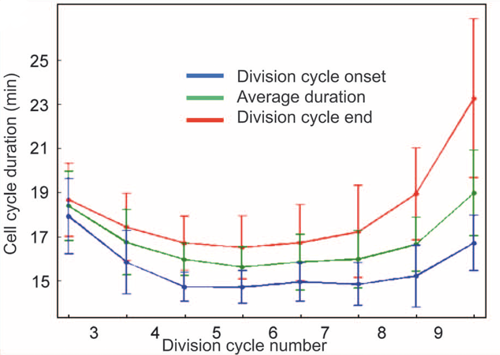
\includegraphics[width=0.4\textwidth]{../../images/Cases_Studies/Case_1_Division/Olivieretal_small.png}
\end{center}
\caption{\textbf{Mean cell cycle duration (green) compared with cycle duration at the beginning (blue) and the end (red) of the division cycle, averaged over six embryos.} Image and caption adapted from \cite{Olivier:2010jz}.}
\label{Case_1_Division_Olivieretal}
\end{figure}

This quantitative study suggests a single dynamic regime for this developmental period, during which the cell cycle length is first shortening then lengthening, although this variation in duration remains quite small (no more than a few minutes). Cell cycle lengthening is supposed to reflect the exhaustion of maternal factors driving the cell cycle progression. It has been postulated that the lengthening of the cell cycle during blastula stages correlates with the ratio of the nucleus size over the cell size. This correlation, however, would not exist any longer by cell cycle 14 \cite{Kane:1996uk}. In Olivier et al. \cite{Olivier:2010jz}, no correlation was found between cycle duration and cell volume for the first 10 cell cycles. Rather, cell cycle length was observed to be dependent on the cell position within the blastoderm. That study proposed that division asynchrony is the rule and increases from cycle 2 to cycle 10 (Fig. \ref{Case_1_Division_Olivieretal2}).
\begin{figure}
\begin{center}
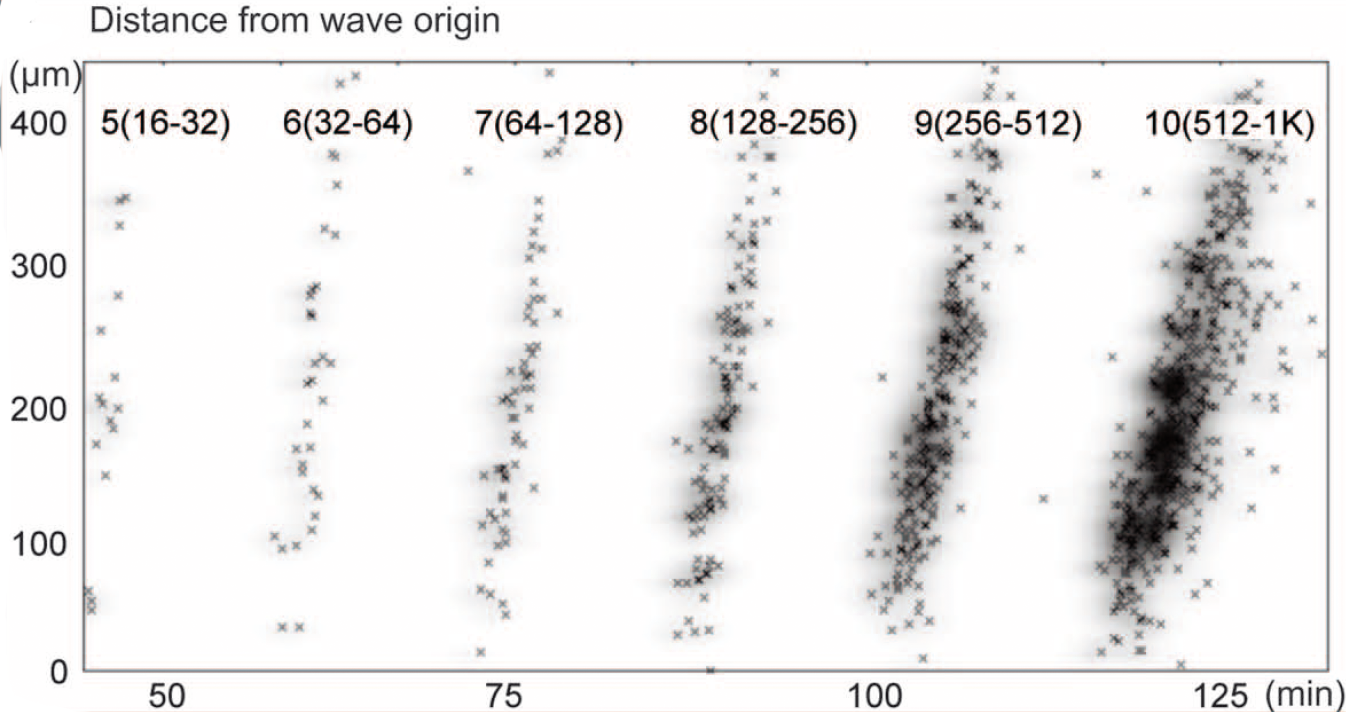
\includegraphics[width=0.4\textwidth]{../../images/Cases_Studies/Case_1_Division/Olivieretal2.png}
\end{center}
\caption{\textbf{Scatter plot of mitosis time as a function of distance to the pseudo-wave origin.} Image and caption adapted from \cite{Olivier:2010jz}.}
\label{Case_1_Division_Olivieretal2}
\end{figure}

This conclusion differs somewhat from the work by Kane and Kimmel \cite{Kane:1993wp} indicating a measurable asynchrony by the midblastula transition only (Fig. \ref{kane_kimmel_1993_cell_cycle}). This discrepancy might however solely reflect the measurements method's sensitivity and precision.
\begin{figure}
\begin{center}
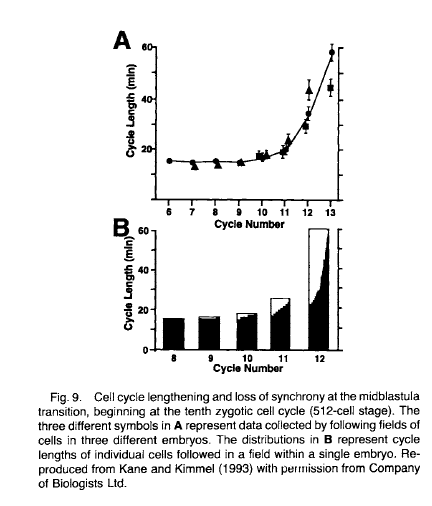
\includegraphics[width=0.4\textwidth]{../../images/Cases_Studies/Case_1_Division/kane_kimmel_1993_cell_cycle.png}
\end{center}
\caption{\textbf{Cell cycle lengthening and loss of synchrony at the midblastula transition.} Adapted from \cite{Kane:1993wp}.}
\label{kane_kimmel_1993_cell_cycle}
\end{figure}

Measurements plotted in Fig. \ref{kane_kimmel_1993_cell_cycle} highlight the progression of cell cycle duration throughout the midblastula transition starting at cycle 10 (512 to 1024 cells, 3 hpf). The cell cycle length increases very significantly as soon the zygotic transcription begins and throughout cycles 11 and 12 \cite{Kane:1993wp}. Cycle 12 should be completed around the sphere stage (4 hpf). According to Kane and Kimmel \cite{Kane:1993wp}, cell cycle lengthening would respond to a single dynamical regime during blastula and early gastrula stages, with the cell cycle length progressing as a linear function of 1/cell volume (Fig. \ref{kane_kimmel_1993_cell_cycle_3}). Such a correlation would lead to a geometric progression of cell cycle lengthening, doubling at each cycle. It should however be noted that this rule does fit with the measurements provided in the paper.
\begin{figure}
\begin{center}
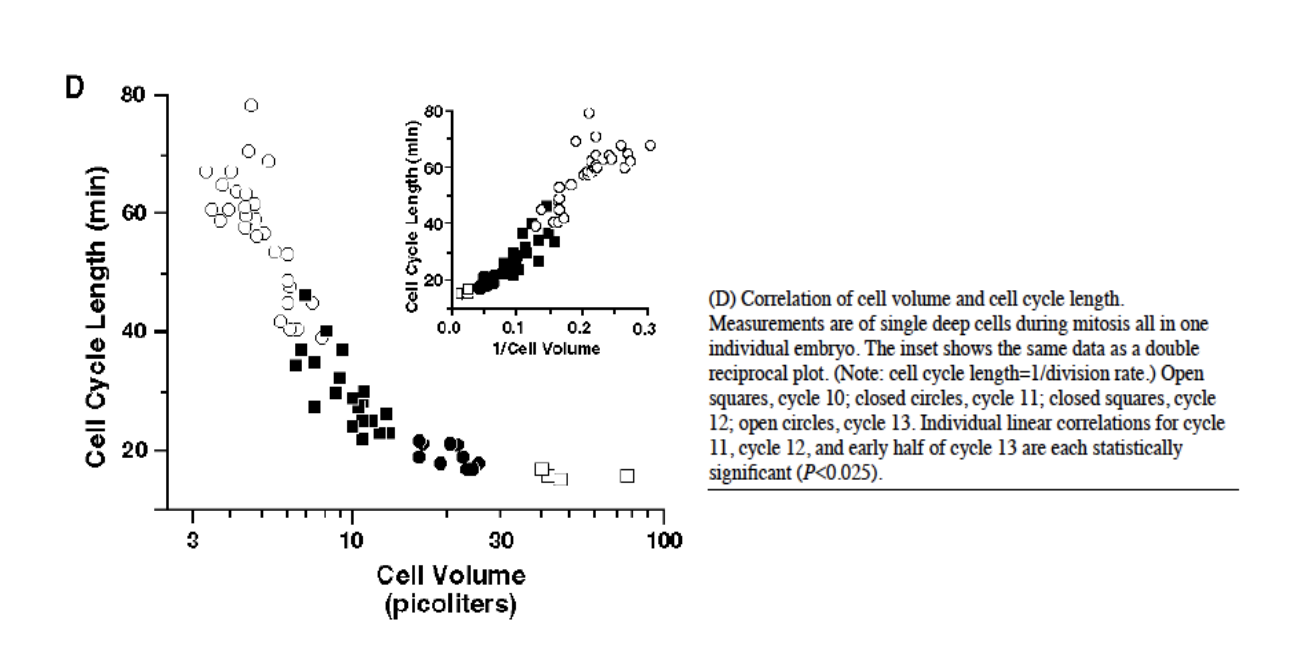
\includegraphics[width=0.8\textwidth]{../../images/Cases_Studies/Case_1_Division/kane_kimmel_1993_cell_cycle_3.png}
\end{center}
\caption{\textbf{Correlation of cell volume and cell cycle length for cycles 10 to 13. } Adapted from \cite{Kane:1993wp}.}
\label{kane_kimmel_1993_cell_cycle_3}
\end{figure}

According to Kane and Kimmel, gastrulation would proceed during cell cycle 14. Cell proliferation during gastrulation continues to slow down dramatically so that, on average, cells divide only once between 6 and 10 hpf. It has also been shown that gastrulation is not impaired by the inhibition of cell divisions. If cell proliferation is indeed required to provide a minimal number of cells for further morphogenetic movements, gastrulation appears quite robust to perturbations of the cell cycle. For example, in \textit{emi1} (\textit{early mitotic inhibitor-1}), homozygous mutant defective in the expression of this negative regulator of the Anaphase Promoting Complex \cite{Zhang:2008gw}, gastrulation and somitogenesis proceed while mitotic activity stopped at the beginning of gastrulation (shield stage 6 hpf).

The state-of-the-art data and analysis leave open a number of questions. First, precise measurements of the cell cycle duration along the cell lineage and other parameters including the cell volume and nucleus volume, when discussing correlations between the cell cycle length and the cell volume or nucleo-cytoplasmic ratio, are lacking except for the first 10 cycles \cite{Olivier:2010jz}. Without precise phenomenological reconstructions, it is very difficult to make relevant hypotheses on the dynamic regimes controlling the cell proliferation rate along the cell lineage. The model proposed by Kane and Kimmel for the progression of the cell cycle duration in 1/V readily leads to a geometric progression rule that should be further tested and discussed. In addition, increasing asynchrony of cell divisions should be better characterized to provide the most precise phenomenology for a further investigation of the underlying mechanisms.
%  ---------------------------------------------------------------------- 


\subsubsection{Hypotheses and Model}
%  ---------------------------------------------------------------------- 


In our model, we make the approximation that through the first 10 divisions, cell cycle length is constant and constrained to reach the 1,000-cell stage by 3 hpf, i.e. at the time of midblastula transition. We are then looking for an appropriate model of cell cycle lengthening and subsequent desynchronization. Our approximation does not exclude, however, that the desynchronization might obey the same rule throughout the first 14 or 15 cell cycles. From the study by Kane and Kimmel \cite{Kane:1993wp}, we understand that the cell cycle duration might slow down according to a geometric progression. Indeed, the authors suggest a progression as a linear function of 1/V. As cells are expected to divide at constant volume until the end of gastrulation, the cell volume should be divided and the cell cycle should double. Yet, as already discussed, this does not match the data (Fig. \ref{kane_kimmel_1993_cell_cycle_2}).
\begin{figure}
\begin{center}
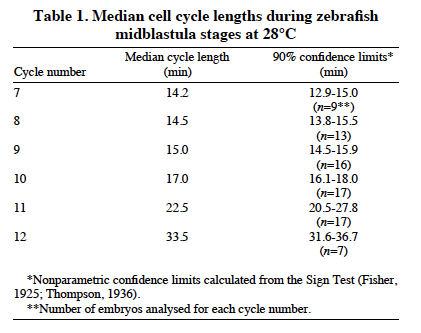
\includegraphics[width=0.4\textwidth]{../../images/Cases_Studies/Case_1_Division/kane_kimmel_1993_cell_cycle_2.png}
\end{center}
\caption{\textbf{Median cell cycle lengths during blastula stages.} Adapted from \cite{Kane:1993wp}.}
\label{kane_kimmel_1993_cell_cycle_2}
\end{figure}

We propose to test two different hypotheses corresponding to either a geometric or an arithmetic progression of cell cycle lengthening. In each model, two parameters determine the cell cycle progression: one for the mean of the distribution and the other for its range. In the following, the length of the cell cycle is denoted by $L_{\mathrm{cc}}$. It is function of an integer value $n$ representing its iteration, e.g. $L_{\mathrm{cc}}(12)$ is the length of the 12$^{\mathrm{th}}$ cell cycle. The iteration from which the cell cycle increases is denoted by $n_{\mathrm{start}}$ and the last iteration by $n_{\mathrm{end}}$. Similarly, the timing of a cell cycle is denoted by $T_{\mathrm{cc}}$.

\paragraph{Geometric progression of the cell cycle}
%  ++++++++++++++++++++++++++++++++++++++++++++++++++++++++++++++++++++++ 


A geometric progression of the cell cycle iteratively multiplies the length of the cell cycle by a value, the \textit{common ratio}, denoted by $r$:

$$\forall n \in \left[ n_{\mathrm{start}}, n_{\mathrm{end}} \right], L_{\mathrm{cc}}(n+1) = r \cdot L_{\mathrm{cc}}(n)$$

We suppose that the common ratio follows a uniform distribution centered on $r_0$ and with a range of $w_r$:

$$r = \mathcal{U}(r_0 - \frac{w_r}{2}, r_0 + \frac{w_r}{2})$$

During the development of a simulated embryo, each cell division requires the generation of a new random common ratio $r$ determined with the parameters $r_0$ and $w_r$. We also make the assumption that the cell cycle length is always increasing after each division, so the common ratio $r$ must be larger than 1. It implies the following constraint on the parameters of the study:

$$w_r \leq 2(r_0 -1)$$
\begin{figure}
\begin{center}
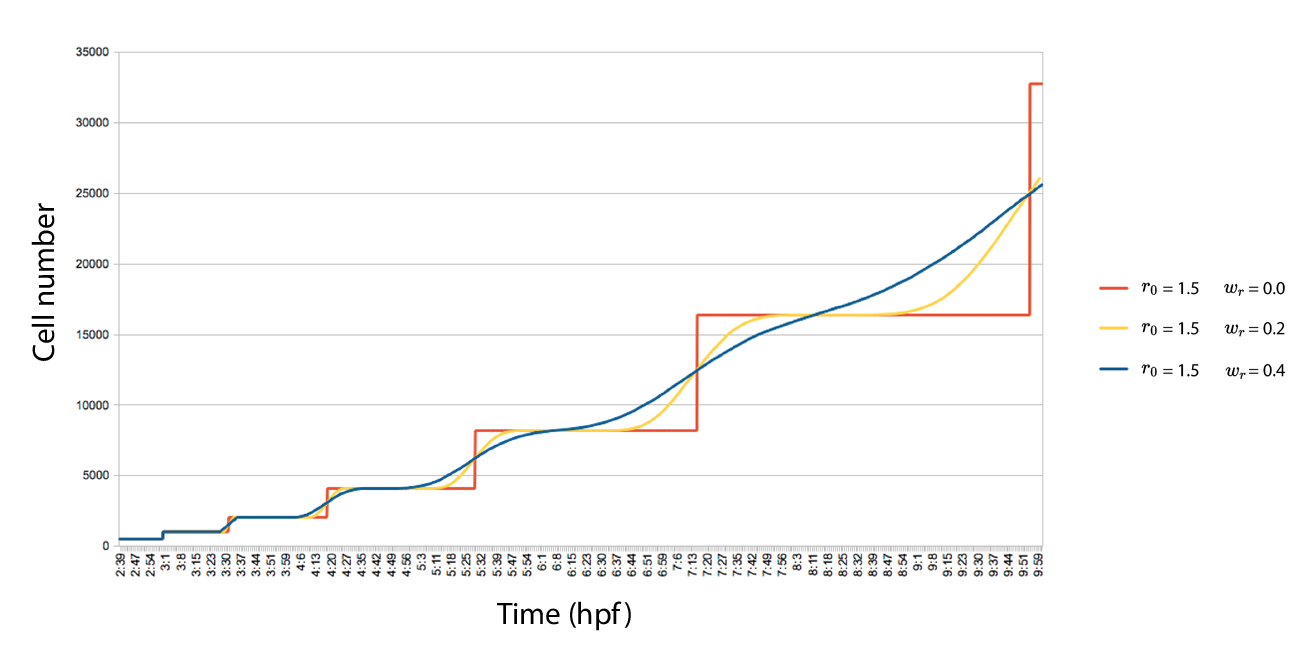
\includegraphics[width=0.8\textwidth]{../../images/Cases_Studies/Case_1_Division/cell_number_plot/cell_number_plot.png}
\end{center}
\caption{\textbf{Theoretical cell number as a function of time of development in the geometric progression scenario.} In ordinate, the number of simulated cells. In abscissa, time of development starting at 2h39. Three geometric progression scenario are plotted. Each of them starts from an initial simulated cell population comprising 512 cells with identical cell cycle length (see text), and identical common ratio ($r_0 = 1.5$). In red, the asynchrony is zero, all cells divide simultaneously at each cycle ($w_r = 0$). In yellow, cell cycles are desynchronizing reasonably at each cycle ($w_r = 0.2$), plateaus are still occurring in between mitosis cycles. In blue, a larger desynchronization ($w_r = 0.4$) leads to a progressive disappearance of the plateau as the cell population increases. }
\label{cell_number_plot_cell_number_plot}
\end{figure}

\paragraph{Arithmetic progression of the cell cycle}
%  ++++++++++++++++++++++++++++++++++++++++++++++++++++++++++++++++++++++ 


An arithmetic progression of the cell cycle iteratively sums the length of the cell cycle by a constant value, the \textit{common difference}, denoted by $d$:

$$\forall n \in \left[ n_{\mathrm{start}}, n_{\mathrm{end}} \right], L_{\mathrm{cc}}(n+1) = d + L_{\mathrm{cc}}(n)$$

As before, we assume that the common difference follows a uniform distribution centered on $d_0$ and with a range of $w_d$.

$$d = \mathcal{U}(d_0 - \frac{w_d}{2}, d_0 + \frac{w_d}{2})$$

During the development of a simulated embryo, each cell division requires the generation of a new random common difference $d$ determined with the parameters $d_0$ and $w_d$. We also make the assumption that the cell cycle length is always increasing after each division, so the common difference $d$ must be larger than 0. It implies the following constraint on the parameters of the study:

$$w_d \leq 2 r_0$$
%  ---------------------------------------------------------------------- 


\subsubsection{Simulation, Parameter Space and Validation}
%  ---------------------------------------------------------------------- 


\paragraph{Cell cycle length measurement through the reconstructed lineage tree}
%  ++++++++++++++++++++++++++++++++++++++++++++++++++++++++++++++++++++++ 


To explore the parameter space and evaluate the fitness of the two hypothesized cell cycle rules (geometric and arithmetic), we manually selected a small population of cells from cell cycle 9 (512-cell stage) at approximately 2h40 hpf and followed them through the lineage tree produced by the reconstruction workflow (described in Chapter 7) until cell cycle 15.


\begin{figure}
\begin{center}
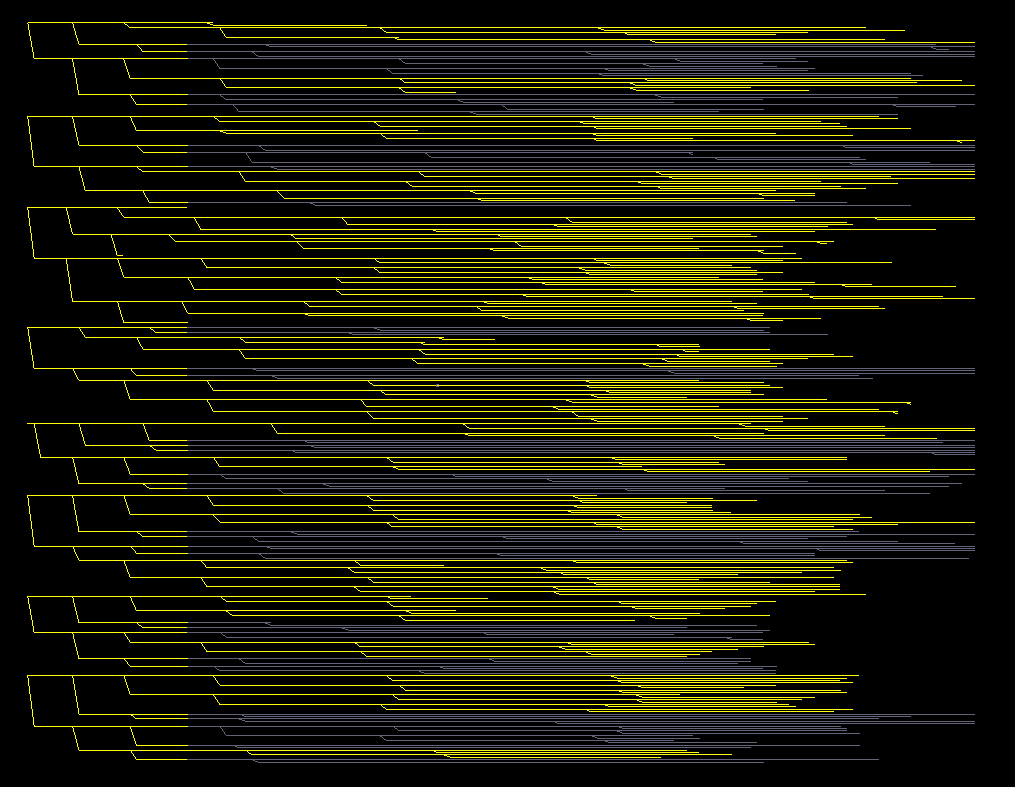
\includegraphics[width=0.9\textwidth]{../../images/Cases_Studies/Case_1_Division/071222bF_t_selection_1_all_T_121224_lineage_tree_no_evl.png}
\end{center}
\caption{\textbf{Lineage tree of the selected cell population.} The selected population consists in eight cells picked at the time of cell cycle 9. At cycle 9 they divide quasi-synchronously (one cell out of the eight divides one time step, i.e. 3 min, after the others). The selected cells contribute to the formation of the EVL. As this differentiated tissue is expected to have a specific cell cycle dynamics (see Case Study 8.4), EVL cells were removed from the selected cell population after division cycle 11. EVL cell lineage removed from the analyzed data is indicated by the grey branches. Cell cycle 11 occurs at the onset of the epiboly at the time of doming, prior to what is usually considered as gastrulation (6 hpf). The selected cells tracking was checked and corrected as far as possible in time.}
\label{Case_1_Division_071222bF_t_selection_1_all_T_121224_lineage_tree_no_evl}
\end{figure}
\begin{figure}
\begin{center}
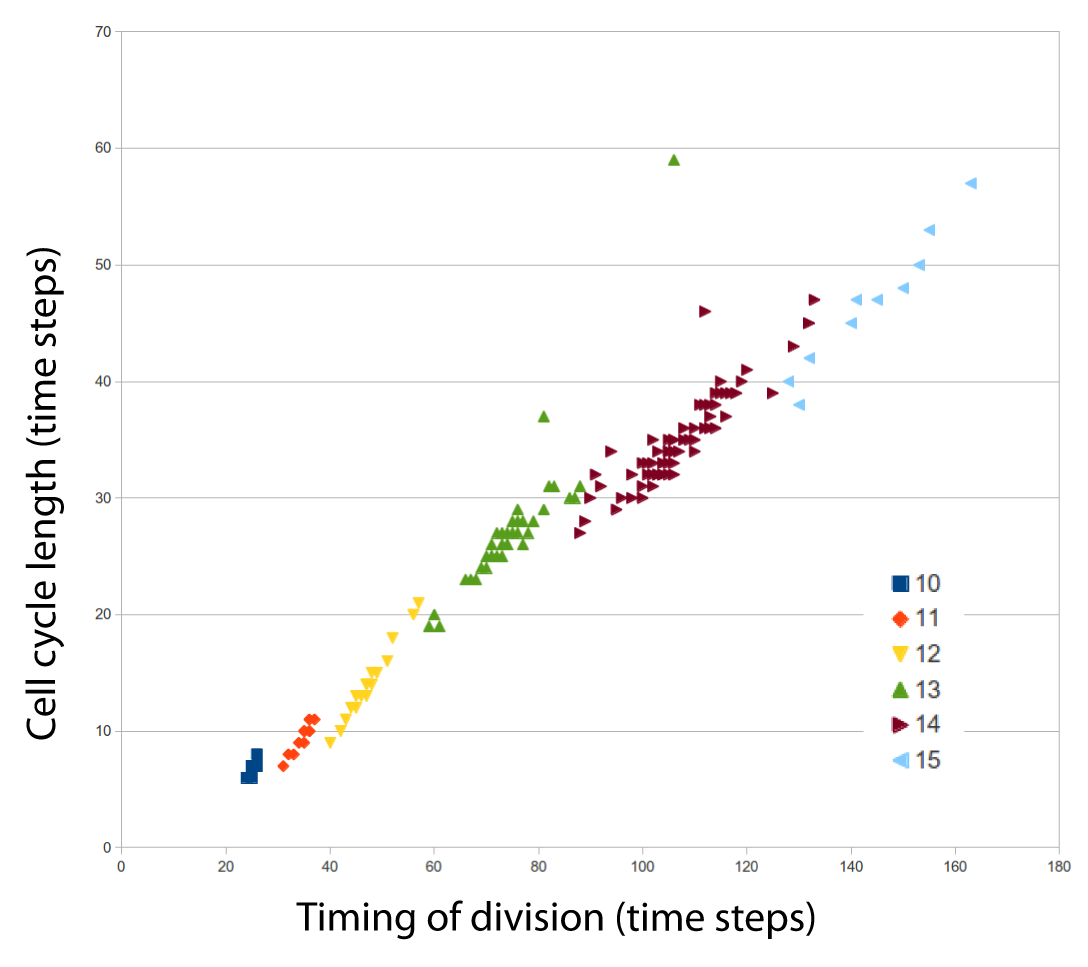
\includegraphics[width=0.9\textwidth]{../../images/Cases_Studies/Case_1_Division/071222bF_t_selection_1_all_T_121224_cellcyclelength_per_generation.png}
\end{center}
\caption{\textbf{Plot of the cell cycle length for cells selected among the deep cells, as a function of the timing of the divisions.} Colors and numbers represent the iteration of the cell cycle as indicated on the right. A cell is plotted at the time of a division as a function of the timing of its mother's division. Timing is indicated in time steps.}
\label{Case_1_Division_071222bF_t_selection_1_all_T_121224_cellcyclelength_per_generation}
\end{figure}


As we do not have the complete data for cell cycle 15, this data is not included in the study. In addition, we interpret the three points that are outside the clouds to be caused by tracking errors that were not found by eye inspection of the raw data. These three points have also been removed from the study.
\begin{figure}
\begin{center}
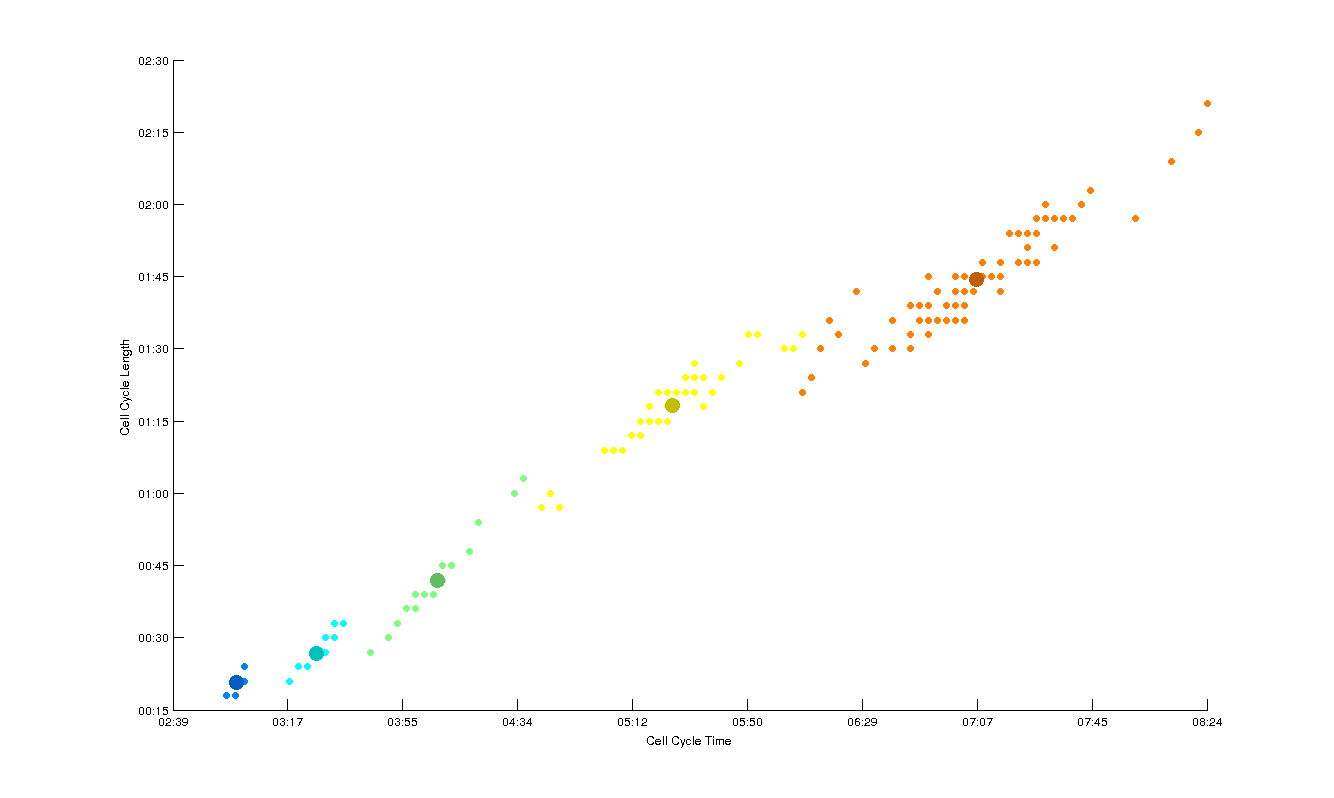
\includegraphics[width=0.95\textwidth]{../../images/Cases_Studies/Case_1_Division/071222bF_t_selection_1_all_T_121224_cellcyclelength_per_generation_MATLAB_mean.png}
\end{center}
\caption{\textbf{Plot of the cell cycle length as a function of the cell cycle time for the cell population selected in the digital specimen.} The blue color represents the $10^{th}$ cell cycle, light blue, the $11^{th}$, green, the $12^{th}$, yellow, the $13^{th}$, and orange, the $15^{th}$. Small dots correspond to single cells at the time of mitosis and large dots are the mean of the division timing for the corresponding cell cycle. The data is the same as Fig. \ref{Case_1_Division_071222bF_t_selection_1_all_T_121224_cellcyclelength_per_generation} without cell cycle 15 and after elimination of the three outliers discussed above. This data is used for confronting live experimental and simulated data.}
\label{071222bF_t_selection_1_all_T_121224_cellcyclelength_per_generation_MATLAB_mean}
\end{figure}

\paragraph{Simulated cell cycles}
%  ++++++++++++++++++++++++++++++++++++++++++++++++++++++++++++++++++++++ 

%  Nous avons besoin ici je pense des films des embryons simules qui correspondent a tes deux types de progression. Tes donnees live sont sorties d'une imagerie 3D+temps, je m'attends a ce que tes donnees simulees sortent d'un film d'embryons simules en developpement. 


We simulated two developments with respectively a geometric progression and an arithmetic progression of the cell cycle length between cycle 9 and cycle 14. To account for the desynchronization of the cell cycles, we took the common ratio and common difference as uniform distributions, as described above. We derived from these simulations the same kind of plot as for the live experimental data (Fig. \ref{071222bF_t_selection_1_all_T_121224_cellcyclelength_per_generation_MATLAB_simu_arrow}). However, unlike for the live experiment, we were able here to plot all the cells of the embryo.
\begin{figure}
\begin{center}
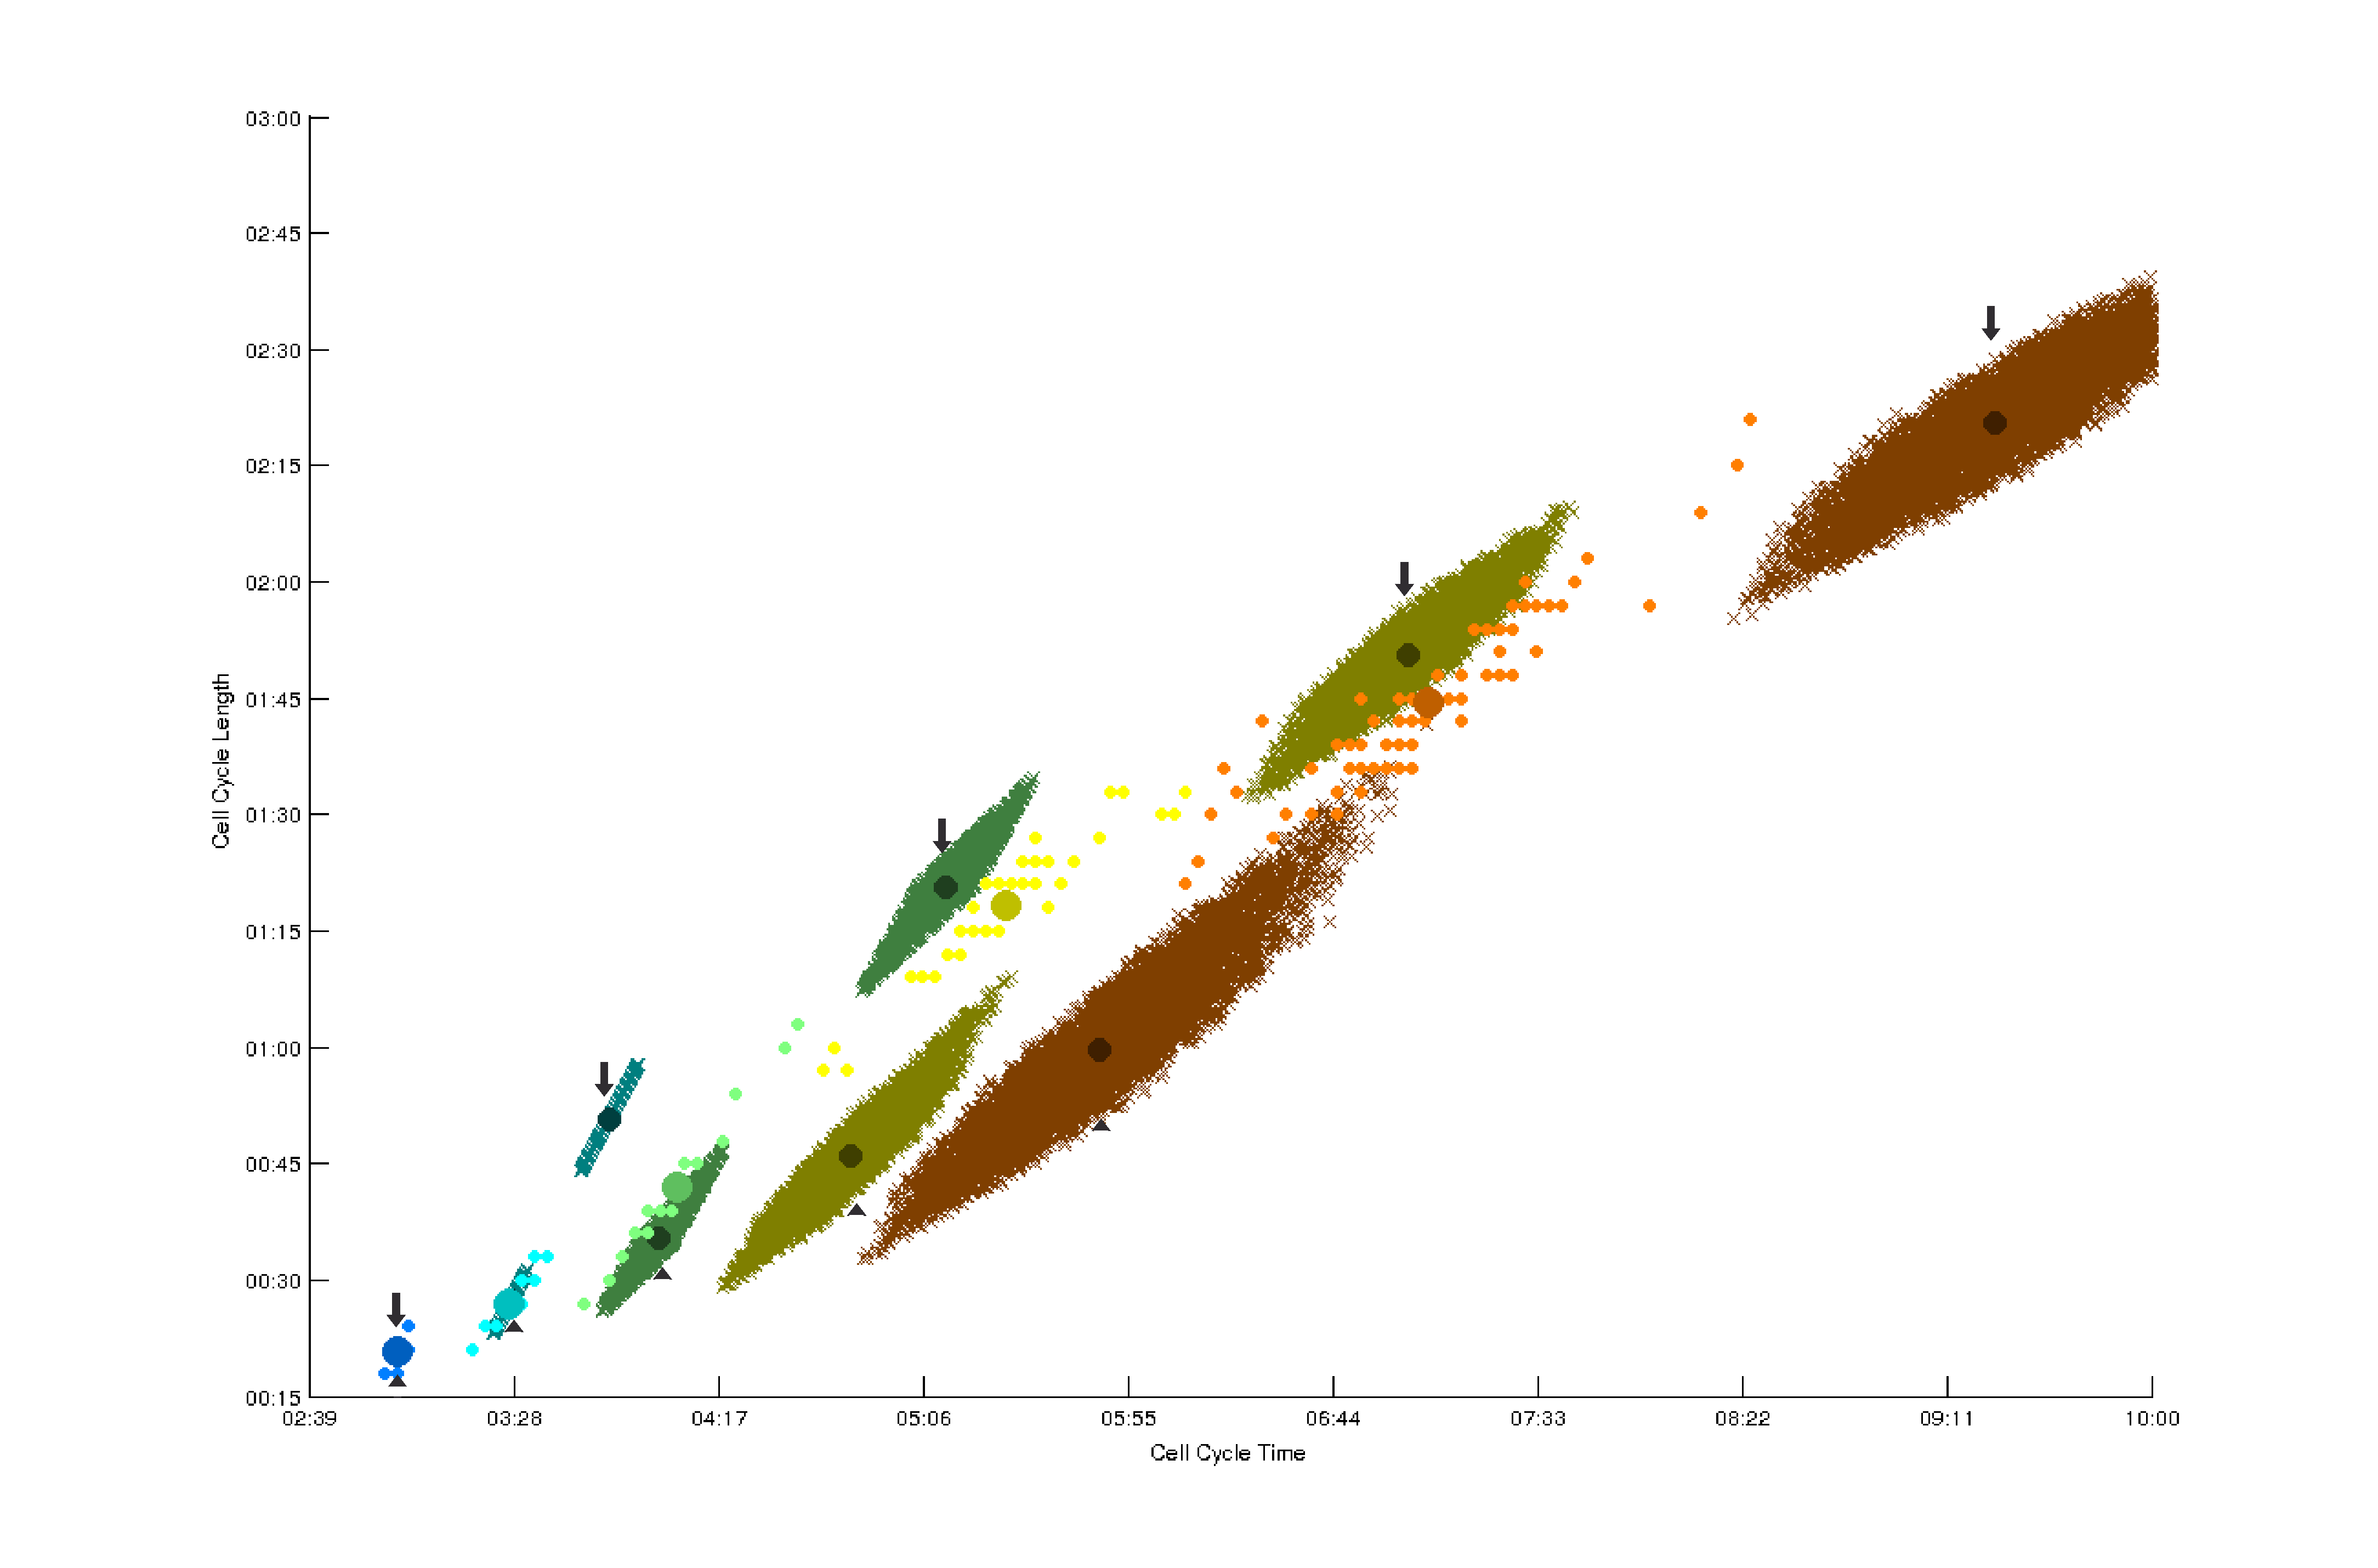
\includegraphics[width=0.95\textwidth]{../../images/Cases_Studies/Case_1_Division/071222bF_t_selection_1_all_T_121224_cellcyclelength_per_generation_MATLAB_simu_arrow.png}
\end{center}
\caption{\textbf{Plot of the cell cycle length as a function of the the cell cycle time for two simulated embryonic developments.} In addition to the live cells plot, we provide two simulated distributions, one corresponding to a geometric progression, indicated by arrowheads ($r_0 = 1.3$ and $w_r = 0.4$, and one corresponding to an arithmetic progression, indicated by arrows ($d_0 = 30 \mathrm{min}$ and $w_d = 14 \mathrm{min}$). For the sake of visualization, we picked here parameters that obviously did not provide the best fitness but kept the clouds separated.}
\label{071222bF_t_selection_1_all_T_121224_cellcyclelength_per_generation_MATLAB_simu_arrow}
\end{figure}

\paragraph{Fitness function}
%  ++++++++++++++++++++++++++++++++++++++++++++++++++++++++++++++++++++++ 


The fitness function used to evaluate the adequacy of the proposed cell cycles is multi-objective. Four objective subfunctions will be evaluated for each set of parameters:
\begin{itemize}
	\item $F_{\mu}(T_{\mathrm{cc}})$, the mean of the cell cycle timing for each generation,
	\item $F_{\sigma}(T_{\mathrm{cc}})$, the standard deviation of the cell cycle timing for each generation,
	\item $F_{\mu}(L_{\mathrm{cc}})$, the mean of the cell cycle length for each generation,
	\item $F_{\sigma}(L_{\mathrm{cc}})$, the standard deviation of the cell cycle length for each generation.
\end{itemize}

All four objectives are expressed through the same type of generic objective function:

$$F_{\mu}(T_{\mathrm{cc}}) = \sum_{n=n_{\mathrm{start}}}^{n_{\mathrm{end}}} \frac{ \left | \mu[T_{\mathrm{cc}}^{\mathrm{s}}(n)] - \mu[T_{\mathrm{cc}}^{\mathrm{v}}(n)] \right |}{\mu[T_{\mathrm{cc}}^{\mathrm{v}}(n)]}$$

$$F_{\sigma}(T_{\mathrm{cc}}) = \sum_{n=n_{\mathrm{start}}}^{n_{\mathrm{end}}} \frac{ \left | \sigma[T_{\mathrm{cc}}^{\mathrm{s}}(n)] - \sigma[T_{\mathrm{cc}}^{\mathrm{v}}(n)] \right |}{\sigma[T_{\mathrm{cc}}^{\mathrm{v}}(n)]}$$

$$F_{\mu}(L_{\mathrm{cc}}) = \sum_{n=n_{\mathrm{start}}}^{n_{\mathrm{end}}} \frac{ \left | \mu[L_{\mathrm{cc}}^{\mathrm{s}}(n)] - \mu[L_{\mathrm{cc}}^{\mathrm{v}}(n)] \right |}{\mu[L_{\mathrm{cc}}^{\mathrm{v}}(n)]}$$

$$F_{\sigma}(L_{\mathrm{cc}}) = \sum_{n=n_{\mathrm{start}}}^{n_{\mathrm{end}}} \frac{ \left | \sigma[L_{\mathrm{cc}}^{\mathrm{s}}(n)] - \sigma[L_{\mathrm{cc}}^{\mathrm{v}}(n)] \right |}{\sigma[L_{\mathrm{cc}}^{\mathrm{v}}(n)]}$$

where $n_{\mathrm{start}}=10$, $n_{\mathrm{start}}=14$, $L_{\mathrm{cc}}^{\mathrm{v}}(n)$ (resp. $T_{\mathrm{cc}}^{\mathrm{v}}(n)$) is the ensemble of cell cycle timing (resp. length) measured on the real embryo at cell cycle $n$, $L_{\mathrm{cc}}^{\mathrm{s}}(n)$ (resp. $T_{\mathrm{cc}}^{\mathrm{s}}(n)$) is the ensemble of cell cycle timing (resp. length) measured on the simulated embryo at cell cycle $n$, $\mu$ is the mean operator and $\sigma$ the standard deviation operator. Each absolute difference is normalized by the value of the experimental measure, such that the contribution of each cell cycle generation's mean or standard deviation has the same influence on the objective function.

These four objective functions are then merged into a global fitness function through a weighted sum method. Applied to the parameter space, this generates four objective landscapes for each proposed model (Fig. \ref{071222bF_t_selection_1_all_T_121224_fitness_geo_ok} and Fig. \ref{071222bF_t_selection_1_all_T_121224_fitness_ari_ok}). As the aim of this study is to compare the two hypothesized cell cycle rules (geometric and arithmetic) through a global fitness function, each landscape value is normalized to contribute equally to the global fitness function. Various methods of normalization can be used \cite{Marler:2004ha}. Here, we simply divide each objective function by the maximum objective function value over both cell cycle rule landscapes:

$$\overline{F} = \frac{F}{\max(F^{\mathrm{geo}}, F^{\mathrm{ari}})}$$

where $F$ stands for any of the above four objective functions. The global fitness $F_{\mathrm{cc}}$ function is then the average of the four normalized objective functions:

$$F_{\mathrm{cc}} = \frac{1}{4}\left(\overline{F_{\mu}}(T_{\mathrm{cc}}) + \overline{F_{\sigma}}(T_{\mathrm{cc}}) + \overline{F_{\mu}}(L_{\mathrm{cc}}) + \overline{F_{\sigma}}(L_{\mathrm{cc}})\right)$$

\paragraph{Fitness landscape}
%  ++++++++++++++++++++++++++++++++++++++++++++++++++++++++++++++++++++++ 

\begin{figure}
\begin{center}
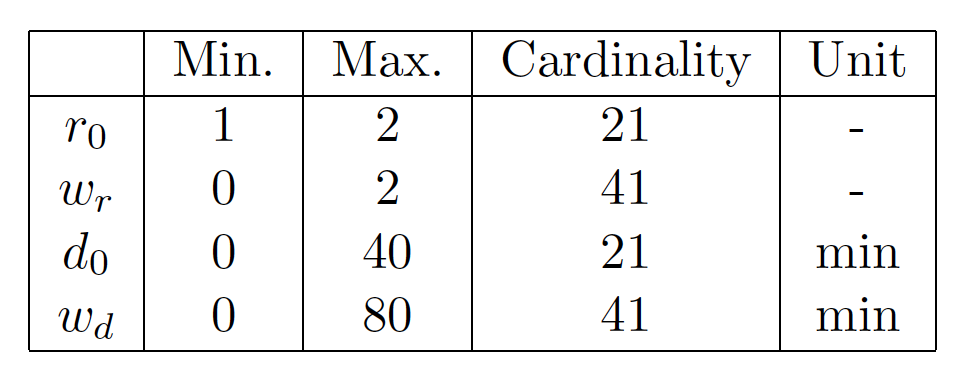
\includegraphics[width=0.5\textwidth]{../../images/Cases_Studies/Case_1_Division/parameter_space_table/parameter_space_table.png}
\end{center}
\caption{\textbf{Ranges, cardinalities and units of the four parameters explored in this study.}}
\label{Case_1_Division_parameter_space_table_parameter_space_table}
\end{figure}
\begin{figure}
\begin{center}
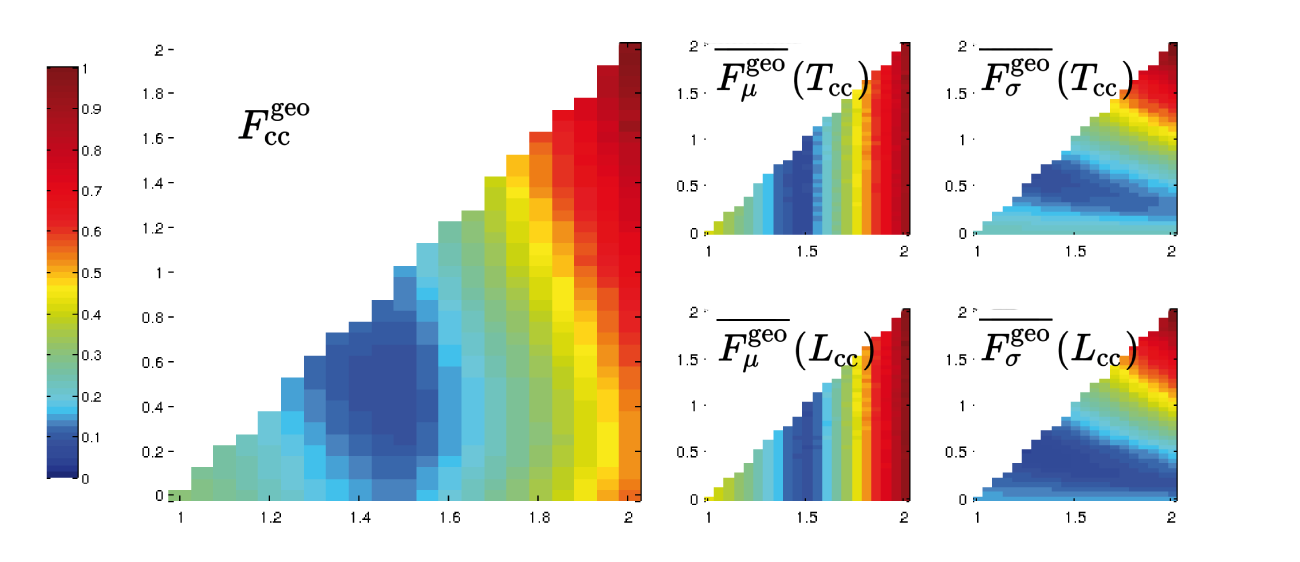
\includegraphics[width=0.95\textwidth]{../../images/Cases_Studies/Case_1_Division/071222bF_t_selection_1_all_T_121224_fitness_geo_ok.png}
\end{center}
\caption{\textbf{Fitness landscapes of the \textit{geometric} progression rule in parameter space.} The left plot is the global fitness landscape. In the right part of the figure: the top left plot is the landscape of the mean of the cell cycle time's normalized objective function $\overline{F^{\mathrm{geo}}_{\mu}}(T_{\mathrm{cc}})$, the top right plot is the landscape of the standard deviation of the cell cycle time's normalized objective function $\overline{F^{\mathrm{geo}}_{\sigma}}(T_{\mathrm{cc}})$, the bottom left plot is the landscape of the mean of the cell cycle length normalized objective function $\overline{F^{\mathrm{geo}}_{\mu}}(L_{\mathrm{cc}})$, the bottom right plot is the landscape of the standard deviation of the cell cycle length normalized objective function $\overline{F^{\mathrm{geo}}_{\sigma}}(L_{\mathrm{cc}})$. The color map of all five plots follows the same color bar presented on the left. Each plot provides the cell cycle distribution center $r_0$ on the abscissa axis and the distribution range coefficient $w_r$ on the ordinate axis. Both parameters are explored in the range presented in Fig. \ref{Case_1_Division_parameter_space_table_parameter_space_table}}
\label{071222bF_t_selection_1_all_T_121224_fitness_geo_ok}
\end{figure}
\begin{figure}
\begin{center}
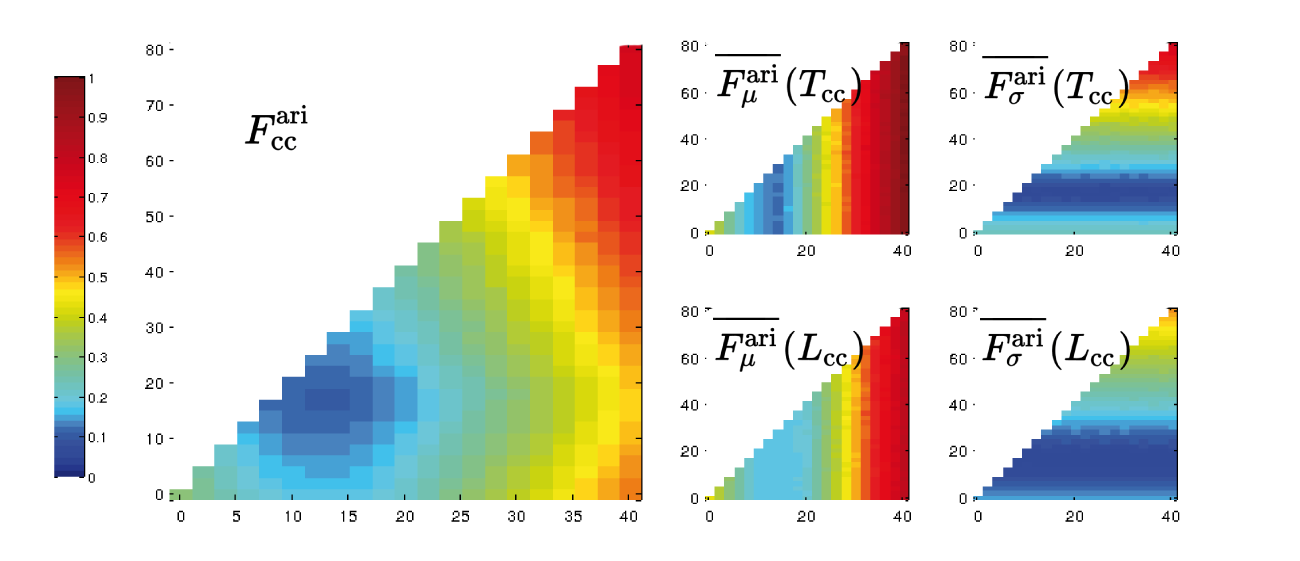
\includegraphics[width=0.95\textwidth]{../../images/Cases_Studies/Case_1_Division/071222bF_t_selection_1_all_T_121224_fitness_ari_ok.png}
\end{center}
\caption{\textbf{Fitness landscapes of the \textit{arithmetic} progression rule in parameter space.} The left plot is the global fitness landscape. In the right part of the figure: the top left plot is the landscape of the mean of the cell cycle time's normalized objective function $\overline{F^{\mathrm{ari}}_{\mu}}(T_{\mathrm{cc}})$, the top right plot is the landscape of the standard deviation of the cell cycle time's normalized objective function $\overline{F^{\mathrm{ari}}_{\sigma}}(T_{\mathrm{cc}})$, the bottom left plot is the landscape of the mean of the cell cycle length normalized objective function $\overline{F^{\mathrm{ari}}_{\mu}}(L_{\mathrm{cc}})$, the bottom right plot is the landscape of the standard deviation of the cell cycle length normalized objective function $\overline{F^{\mathrm{ari}}_{\sigma}}(L_{\mathrm{cc}})$. The color map of all five plots follows the same color bar presented on the left. Each plot provides the cell cycle distribution center $d_0$ on the abscissa axis and the distribution range coefficient $w_d$ on the ordinate axis. Both parameters are explored in the range presented in Fig. \ref{Case_1_Division_parameter_space_table_parameter_space_table}}
\label{071222bF_t_selection_1_all_T_121224_fitness_ari_ok}
\end{figure}
\begin{figure}
\begin{center}
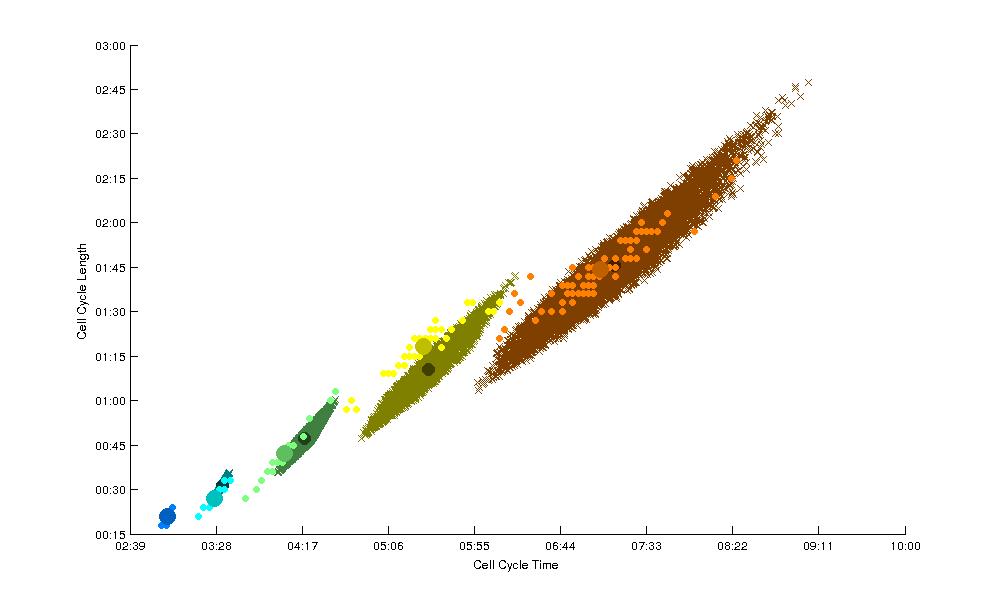
\includegraphics[width=0.95\textwidth]{../../images/Cases_Studies/Case_1_Division/071222bF_t_selection_1_all_T_121224_best_fitness_geo_c1_1.5_c2_0.4.png}
\end{center}
\caption{\textbf{Plot of the cell cycle length $L_{\mathrm{cc}}$ as a function of the cell cycle time $T_{\mathrm{cc}}$ for the simulated embryonic development with the best set of parameters for the \textit{geometric} progression rule.} This phenotype has also the best fitness of this study ($r_0 = 1.5$, $w_r = 0.4$).}
\label{071222bF_t_selection_1_all_T_121224_best_fitness_geo_c1_1.5_c2_0.4}
\end{figure}
\begin{figure}
\begin{center}
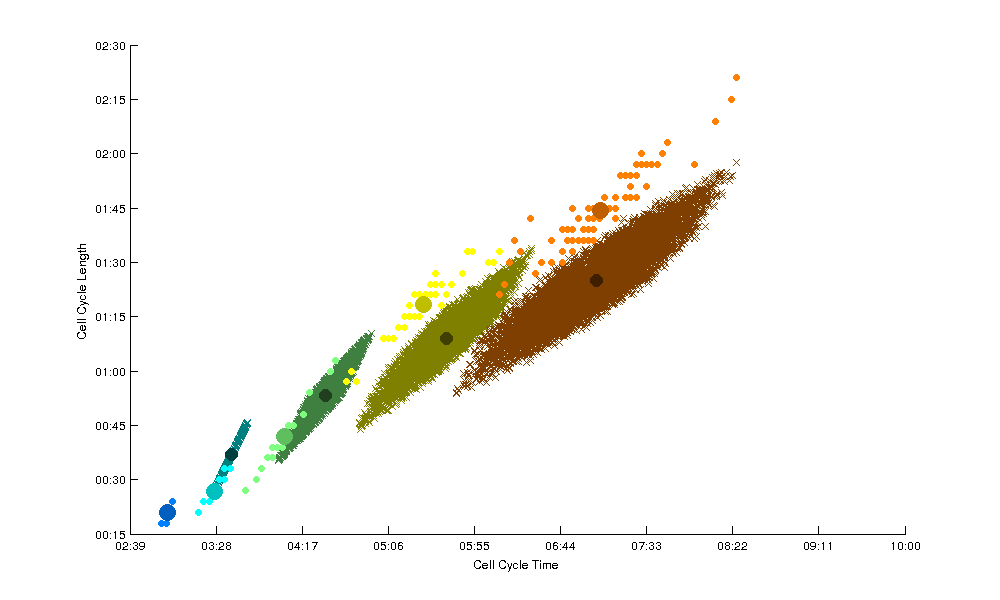
\includegraphics[width=0.95\textwidth]{../../images/Cases_Studies/Case_1_Division/071222bF_t_selection_1_all_T_121224_best_fitness_ari_c1_140_c2_180.png}
\end{center}
\caption{\textbf{Plot of the cell cycle length $L_{\mathrm{cc}}$ as a function of the cell cycle time $T_{\mathrm{cc}}$ for the simulated cells generated with the best set of parameters for the \textit{arithmetic} progression rule.} This phenotype corresponds to the following parameters: $d_0 = 14\,\mathrm{min}$, $w_d = 18\,\mathrm{min}$.}
\label{071222bF_t_selection_1_all_T_121224_best_fitness_ari_c1_140_c2_180}
\end{figure}
%  ---------------------------------------------------------------------- 


\subsubsection{Discussion}
%  ---------------------------------------------------------------------- 


Although the best fitness is realized by the geometric progression, the differences between the real and the simulated phenotypes derived from the two rules are rather close. These values would become more clearly distinct with a larger number of cycles, but this would not be very meaningful biologically, as the regulation of cell proliferation is expected to diversify at later stages and become dependent on cell location and/or lineage.

The best fitness for the arithmetic progression rule does not perform well for the mean time of each cell generation (Fig. \ref{071222bF_t_selection_1_all_T_121224_fitness_ari_ok} bottom left small plot). Thus the overall performance could have been different, i.e. resulting in a slight advantage for the geometric progression model, if the mean objective functions had been assigned a higher weight than the standard deviation functions in the global fitness expression $F_{\mathrm{cc}}$.

Interestingly, the hypothesis of a geometric progression was proposed by Kane. However, this author hypothesized a progression function of 1/V, meaning a common ratio of 2, assuming that at each cell division the cell volume is divided by 2 until the end of gastrulation. Kane's experimental data was not consistent with a common ratio of 2, however, and our best fitness suggests a common ratio of 1.5 instead. If the global cell volume conservation hypothesis was not correct, we could reconcile the two studies and calculate the expected volume evolution.

To account for the desynchronization of cell divisions, the common ratio and common difference for the geometric and arithmetic progressions were assumed to obey uniform distributions. This was an ad hoc choice and the possibility that other distributions would provide better fitness should also be explored. In addition, we simplified the system by assuming the first 9 cycles synchronous. Although this might be considered a reasonable approximation, in fact consistent with our data since our 8 cells divided almost synchronously at cycle 9, this might also hide other important features of the system. The point is that our model is probably more helpful to analyze the desynchronization dynamics, and decide whether it fits different regimes throughout the first 14 or 16 cell cycles or whether, on the contrary, the same type of distribution is suitable to evaluate the dispersion of division times. To test this hypothesis, we might rely on the measurements provided by Olivier et al., which indicate that asynchrony starts at cycle 2 and increases through successive cycles.

\subsection{Shaping the zebrafish gastrula  }

  We aim at documenting the rules in terms of cell-cell interactions and cell-yolk interactions that shape the zebrafish blastula. As shown from previous work \cite{Olivier:2010jz}, by the 16-cell stage, the 4 central cells tend to divide more orthogonal to plane tangent to the sphere, leading to a two layers blastoderm. Through successive divisions, the blastoderm acquires an increasing hight over the yolk until the high stage from which it seems to start flattening, giving rise to the so-called sphere stage (Fig. \ref{Case_2_Cleavage_kimmel_1995}).   
\begin{figure}
\begin{center}
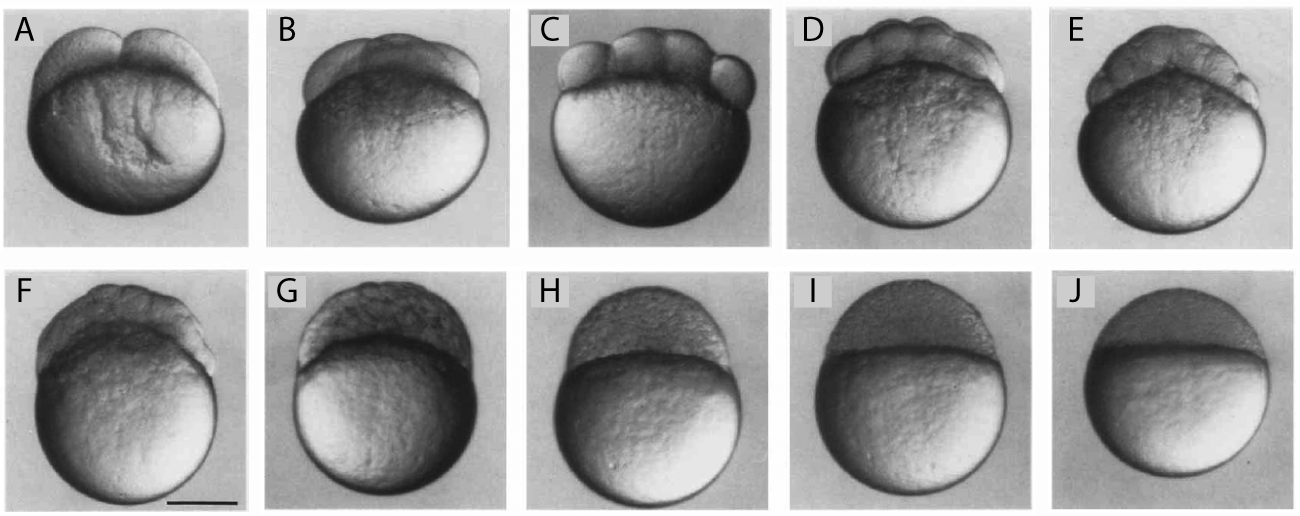
\includegraphics[width=0.7\textwidth]{../../images/Cases_Studies/Case_2_Cleavage/kimmel_1995.png}
\end{center}
\caption{\textbf{Cleavage and blastula period.} From zfin.org, Kimmel et al. Developmental Dynamics 203:253-310 (1995) \cite{Kimmel:1995kn}, Top panel : Embryos during the cleavage period. Face views, except for B, which shows the embryo twisted about the animal-vegetal axis, roughly 45 degrees from the face view. A: 2-cell stage (0.75 h). B: 4-cell stage (1 h). C. 8-cell stage (1.25 h). D: 16-cell stage (1.5 h). E: 32-cell stage (1.75 h). F. 64-cell stage (2 h). Scale bar: 250 µm. Bottom panel : Face views of embryos during the blastula period. A: 256-cell stage (2.5 h). B: high stage (3.3 h). C. transition between the high and oblong stages (3.5 h). D. transition between the oblong and sphere stages (3.8 h). E: dome stage (4.3 h). F. 30percent-epiboly stage (4.7 h). Scale bar: 250 µm.}
\label{Case_2_Cleavage_kimmel_1995}
\end{figure}
\begin{figure}
\begin{center}
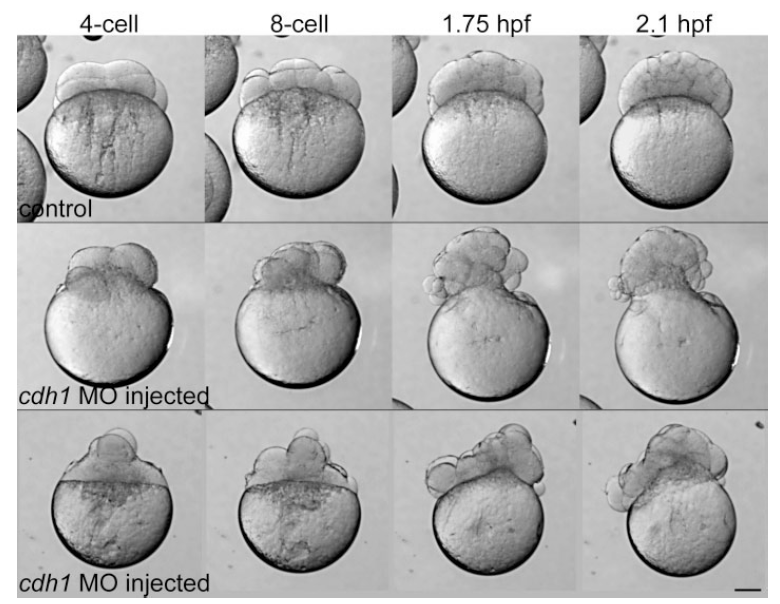
\includegraphics[width=0.7\textwidth]{../../images/Cases_Studies/Case_2_Cleavage/babb_2004.png}
\end{center}
\caption{ajout julien. from \cite{Babb:2004kx}}
\label{Case_2_Cleavage_babb_2004}
\end{figure}

\subsubsection{Hypotheses and Model  }

  We hypothesize that until early blastula stages (high stage), blastoderm shaping arises from cell proliferation, cell division orientation, cell-cell and cell-yolk attraction and repulsion with negligible intrinsic cell motility. Cell proliferation at cleavage and blastula stages have been discussed in the previous section (8.2). Cell division orientation has been quantified \cite{Olivier:2010jz}. At first orthogonal to each other, division planes are described to become more and more randomly oriented. We however expect stronger biomechanical constraints at the blastoderm surface to correlate with biased cell division orientation. Division orientation in the outmost cell layer of the blastoderm distinguishes the EVL (enveloping layer differentiating at the surface of the embryo to form and epithelium réf XXXX) and inner cell lineages and the EVL is expected to be a close compartment at the sphere stage. EVL cells behavior will be investigated in the section 8.4. Cell divisions at the blastoderm yolk interface lead to the formation of the yolk syncytial layer (YSL) around cell cycle 9 (Ref XXX).  

  We hypothesize that from the 8-cell stage until the high-stage, and thus before the differentiation of the EVL, cell-cell and cell-yolk attraction and repulsion are the major parameters underlying blastoderm shaping with a single dynamical regime. We expect by exploring the parameter space defined by the corresponding 4 parameters to find the conditions for shaping the blastoderm according to the quantitative data obtained from live imaging. 

\subsubsection{Simulation, Parameter Space and Validation }

  Prior to a more systematic exploration of the 4D parameter space defined by the cell-cell and cell-yolk attraction, we performed a first confrontation of reconstructed and simulated data with a first set of parameters chosen to provide blastoderm width and height roughly fitting the observations from Fig. \ref{Case_2_Cleavage_kimmel_1995}. We implemented the simultaneous visualization of raw and simulated data with the experimental data from \cite{Olivier:2010jz}. Three data sets from this paper with IDs 081014h, 080917h and 081024h provided live imaging of zebrafish embryos throughout the first 10 cell divisions with THG signal as shown in Fig. \ref{Case_0_Yolk_THG_thg} and SHG signal revealing mitotic spindles. In addition to the reconstructed cell lineage for each of these data sets, the paper proposes a prototypic embryo calculated from 6 different specimens by averaging cell dipoles length at the time of cell division and cell division orientation.   


  Measure 1: is based on the calculation of 3D alpha-shapes. At each time step, we compute (from CGAL http://www.cgal.org/) the 3D alpha-shape from the embryo cell center set. 

  Measure 2: is based on the calculation of 2D alpha shapes. The latter is achieved by projecting by revolution around the AV axis, each cell position on a half plane delimited by the animal-vegetal (AV) axis ((Fig. \ref{Case_2_Cleavage_schematics_lowres})). This operation allowed us to compute a 2D alpha-shape of the projected centers providing measurements easier to analyze than the 3D alpha-shape.  
\begin{figure}
\begin{center}
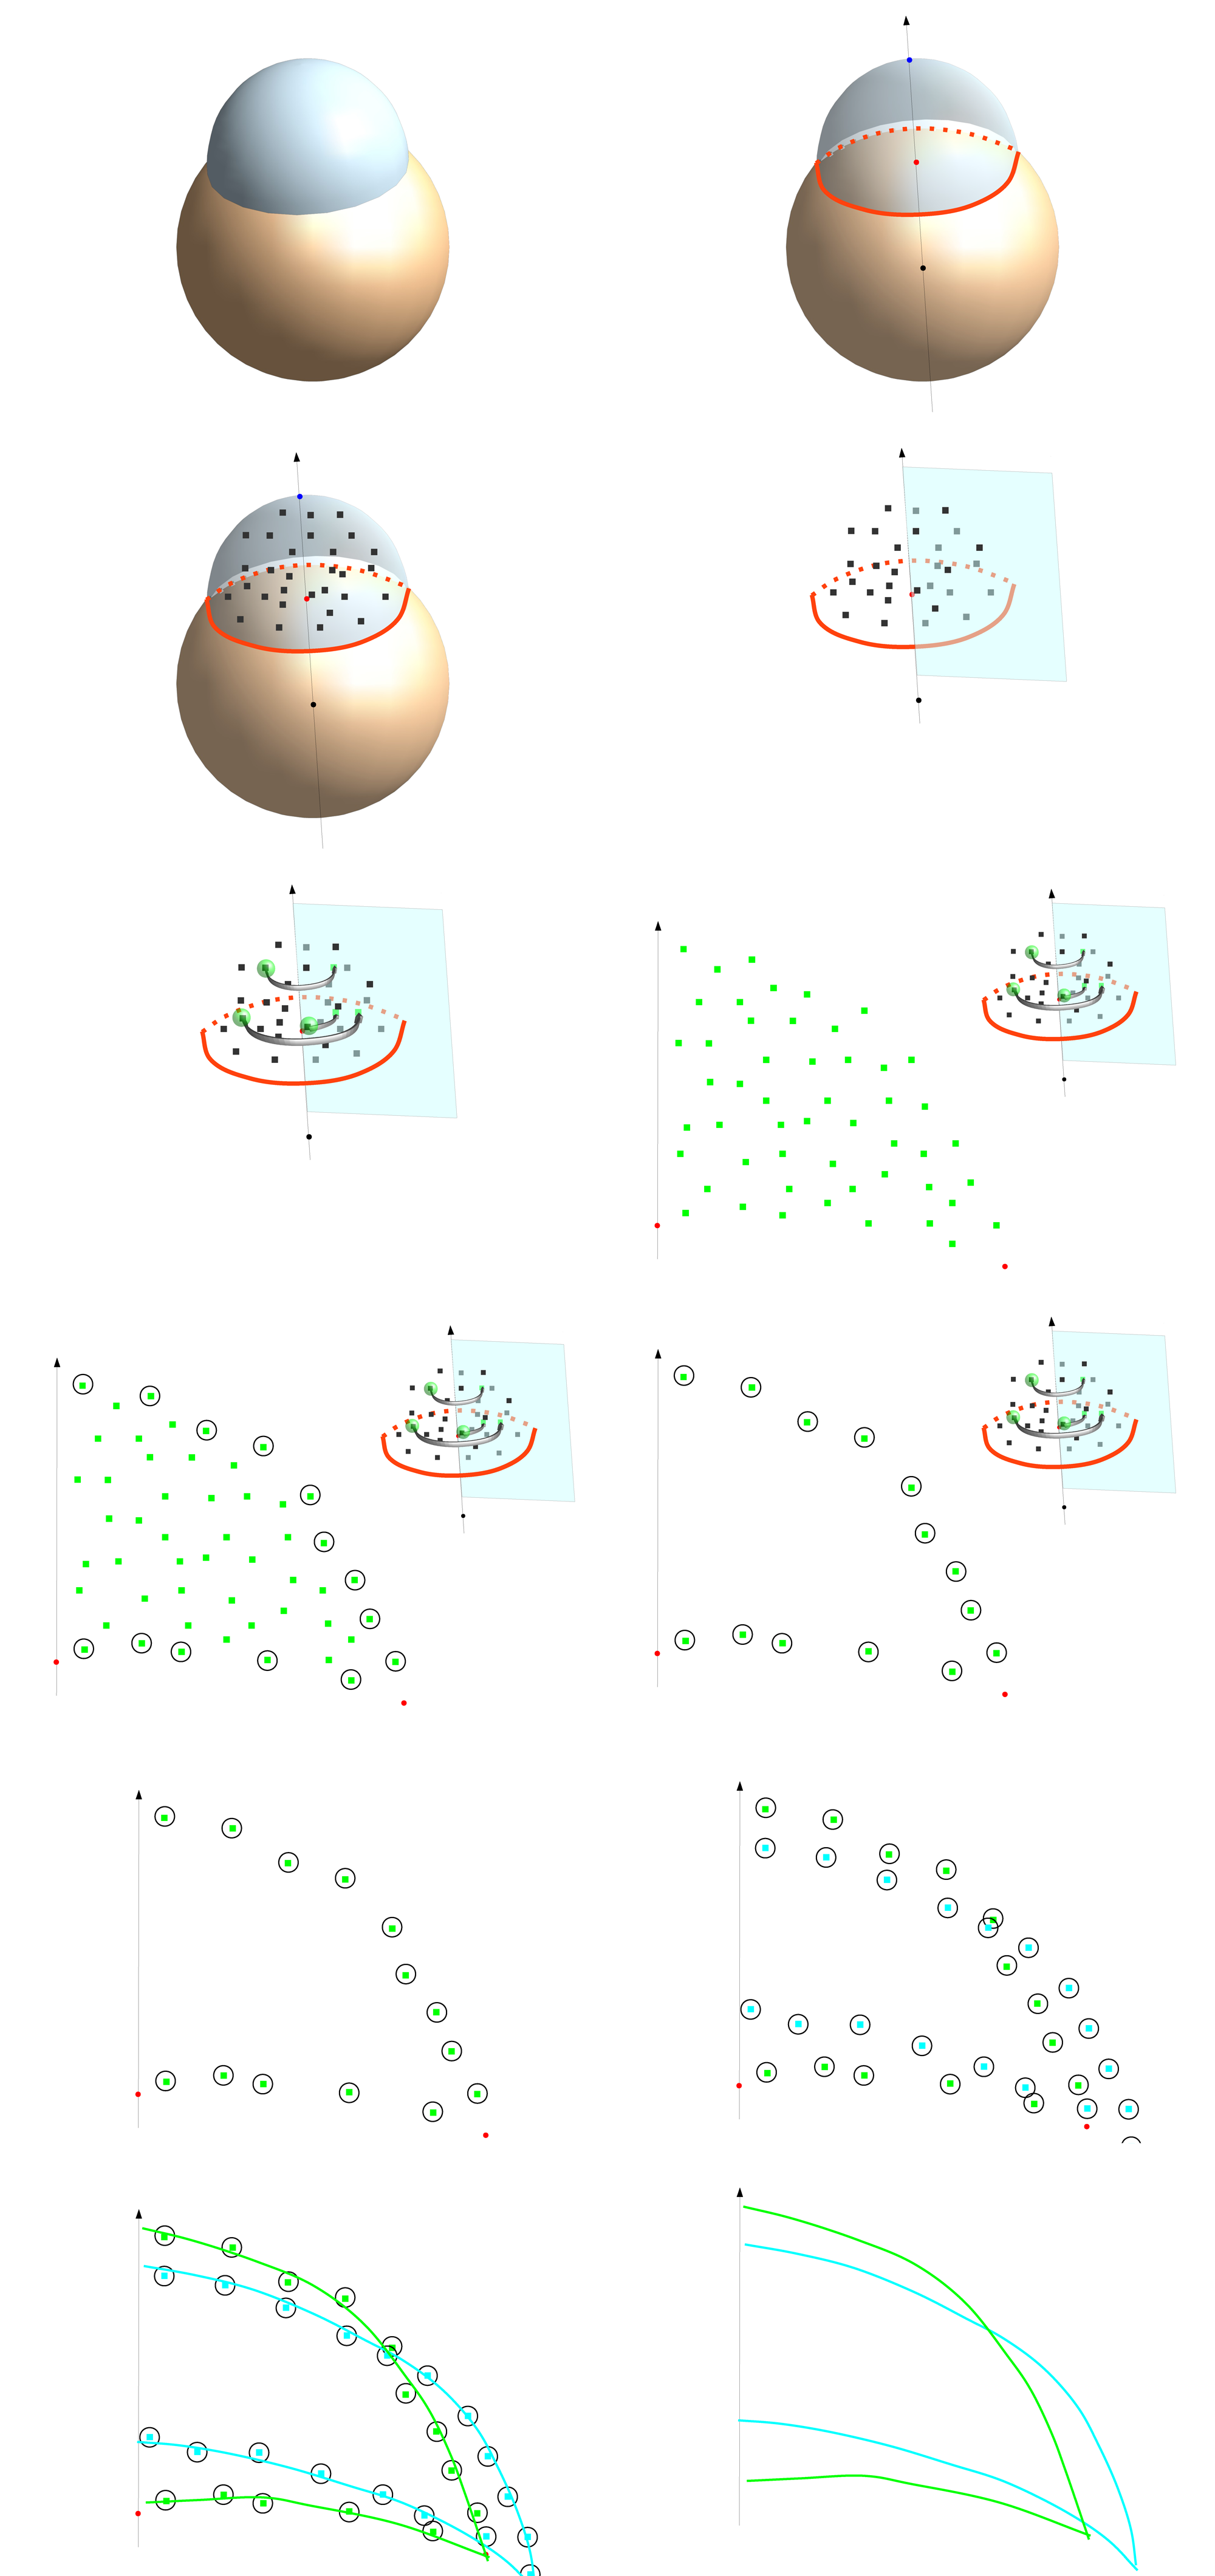
\includegraphics[width=0.7\textwidth]{../../images/Cases_Studies/Case_2_Cleavage/schematics_lowres.png}
\end{center}
\caption{\textbf{A 2D alpha shape strategy for assessing the embryo shape evolution.}}
\label{Case_2_Cleavage_schematics_lowres}
\end{figure}

  A possible measurement to characterize the embryo shape and then compare different embryos is to infer the blastoderm contours, both to get its outside surface and inner surface contacting the yolk. Each curve can be described with a limited number of parameters and we can then predict the shape changes through the evolution of these parameters. This strategy is relevant to characterize both the embryo shape evolution and shape differences between two embryos at the same stage.  

\subparagraph{Fitness Function}

  We propose one fitness function for each type of measurement:  

  Fitness from measure 1 is provided by counting the number of cells from the simulated data set which are outside the alpha-shape of the experimental data set and vice versa. In the best case, the sum of these "outside" centers is null. This sum will be the fitness function for this measure.   

  Fitness from measure 2 is provided by the sum of the differences between the parameters describing the outside and inside curves fitting the blastoderm shape.  

\subsubsection{Discussion  }

   The proposed measures and fitness are currently implemented. Alternatively to the 2 measures proposed, a third one might be implemented and used. We should be able to get from the BioEmergences reconstruction workflow the algorithmic segmentation of the outside and inside surface of the blastoderm from 3D+time imaging of live embryos either imaged with THG or by 2PEF of fluorescently stained cell membranes. This strategy should provide the best approximation (validated by eye inspection) of the blastoderm shape.   

  We expect from this study an optimal shape of the blastoderm that will be used as an initial condition for assessing the properties underlying further development (doming and epiboly). 

  We also expect from this quantitative study of the blastoderm evolution, some indication of the homogeneity of the process. In other words we should be able to propose whether the blastoderm shape evolution goes through different phases, possibly indicating changes at a more microscopic level in terms of cell adhesion, cell tension, cell intrinsic motility, cell yolk interaction, EVL differentiation. 

\subsection{Cell behaviors in the enveloping cell layer compartment  }

  The enveloping cell layer differentiating during blastula stages has been long hypothesized to be an extra embryonic compartment. Recent studies rather suggest a striking parallel between EVL and mammals epidermis (Ref XXXX). EVL through differentiation steps reinforces its epithelial properties. EVL biomechnical properties are expected to be essential for further gastrulation steps where EVL is hypothesized to stand increasing tension.  

\textbf{Intuition adeline:}
\begin{itemize}
	\item moins de division au pole animale qu'a la marge
	\item divisions simultanée avec les voisines
\end{itemize}

\textbf{EVL cell growth}

  Fundulus -> nice picture in Fink, R. & Cooper, M., 1996. Apical membrane turnover is accelerated near cell–cell contacts in an embryonic epithelium. Developmental Biology, 174(2), pp.180–189. \cite{Fink:1996un}
\begin{figure}
\begin{center}
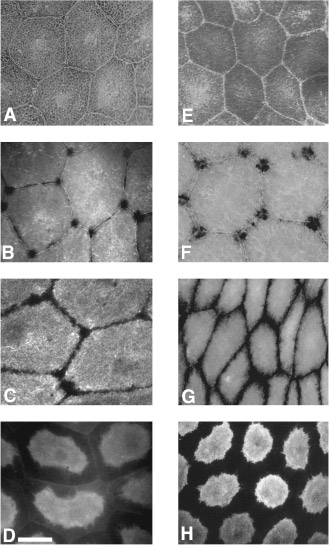
\includegraphics[width=0.4\textwidth]{../../images/Cases_Studies/Case_3_EVL/growth/fink_1996.png}
\end{center}
\caption{Regional membrane turnover within the apical membranes of Fundulus enveloping layer cells. Pairs of photographs showing the temporal progression of membrane turnover (seen as loss of fluorescence) of EVL cells labeled with fluorescent lectin (A–D) and lipid (E–H). Embryos stained with fluorescent lectin initially show a uniform pattern of fluorescence \cite{Fink:1996un}}
\label{growth_fink_1996.png}
\end{figure}

\subsubsection{Hypotheses and Model }

   see Fukazawa, C. et al., 2010. poky/chuk/ikk1 is required for differentiation of the zebrafish embryonic epidermis. Developmental Biology, 346(2), pp.272–283. \cite{Fukazawa:2010bh}

   see Dodd, M.E. et al., 2009. The ENTH domain protein Clint1 is required for epidermal homeostasis in zebrafish. Development, 136(15), pp.2591–2600. \cite{Dodd:2009hf}

   see Goonesinghe, A. et al., 2012. Desmosomal cadherins in zebrafish epiboly and gastrulation. BMC developmental biology, 12, p.1. \cite{Goonesinghe:2012di}
\begin{itemize}
	\item From which time step do we suppose that the 2 populations remain separated ?
\end{itemize}

\textbf{Model:}

   Formation at cycle N:  

   When the division cycle reaches its N_evl_formation th occurence (N_evl_formation  = ), the external cells perform a radial division (normal to the embryo surface) and the external (internal) daughter cell become part of the EVL (IC) population. The externality property is determined by an topological method called "alpha-shaping". The initial EVL lateral radius R_lat is equal to the initial zygote radius divided by the 2^(numgeneration / 3) so the same radius has its sister IC. The apico-basal radius Rap is computed to conserve the yolk volume .5*(4/3)*PI*Ric0^3 * (1/2)^(numgeneration) divided by the surface of the cell (PI * Rlat^2)  

   Mechanical equilibrium: transfer IC->EVL, EVL->IC  

   For a given period of time after the EVL formation, the cell may be transfer between the two population in both direction (IC->EVL, EVL->IC). The criteria for the transfer is based on geometrical consideration (alpha shaping).    The dimension of the EVL->IC conversion gives a regular radius of its generation, the inverse conversion gives a regular Rlat for its generation and the Rab accordingly (see initrialization)  

   size control:   

   "cylindrical" cell -> two dimensional parameters: R_lateral and R_apicobasal (PartRadius and PartRadius(i+NUMEVLCELLmax))  

   volume is supposed constant -> V = Rl^2 * Rap  

   Initially... params_const.EVLPartRadiusLat0...  

   cell pressure:  

   The cell pressure/tension is approximated by the average of the force intensity applied on it.  

   Attention, discussion: pas de division par la surface... et la moyenne annule complétement les assymetries dans l'orientatino des forces. example pression > 0 selon un axe, tension > 0 selon l'axe orthogonale -> moyenne nulle...  

   cell growth :  

   if the pressure is above a given threshold (mecha_params.EVLgrowthTheshold), the lateral radius R_lateral is inrcreased by a given amount (Rlat * params_const.EVL_growth_ratio_lateral = 1.01 * Rlat) and, to conserve the volume, the apico-basal radius R_ap is decreased (Rap = Rap / (params_const.EVL_growth_ratio_lateral*params_const.EVL_growth_ratio_lateral))  

   cell cycle:  

   if the cell lateral radius is above a given threshold (mecha.params.EVLSiveLimit * params_const.EVLPartRadiusLat0) (and if the EVL cell is not in the mphase), a division is triggered.   

   Cell division:  

   The daughter cells have identical size, they maintain their apicobasal radius and the lateral radius is reduced by factor (1/2)^(1/2) to have Vdaugthr = (1 / 2) Vmother  

   The axis of division is selected random in the tangential plane.  

   Cell mechanics  

   -> in between EVL cells  

   -> with the deep cells  

   -> with the yolk  

   -> margin   

\subsubsection{Simulation, Parameter Space and Validation }

   We have implemented standard epithelium measure (see Escudero, L.M. et al., 2011. Epithelial organisation revealed by a network of cellular contacts. Nature communications, 2, p.526. link \cite{Escudero:2011cv}) ie:  
\begin{itemize}
	\item cell area
	\item Degree of a node
	\item clustering coefficient
	\item average degree of neighbors
	\item histogram
\end{itemize}

   Each measure can be spatially discriminated through a mosaic of zones along the Animal-Vegetal axis and the Antero-Posterior axis (see video below).  



\subsubsection{Discussion  }

\subsection{Intercalation Patterns  }

  Introduction du case study (+ celle la thèse): 

  le modèle permet de dépasser la simple observation des cinématiques (vitesses, pattern intercalation) en postulant une mécanique élémentaire sous-jacente. 

  Intercalations (en tant que cinématique) are mandatory. 

  different episodes 
\begin{itemize}
	\item from high -> sphere
	\item from sphere -> shield
	\item from shield -> end of gastrulation (plusieurs phases au cours des dernière phases)
\end{itemize}

  2 type d'intercalation 
\begin{itemize}
	\item radial
	\item mediolateral
\end{itemize}

  meme si grands nombres d'étude dans la litterature, il n'existe pas d'études quantitatives de la contribution de ces diff type d'intercalation, contribution temporellement regionalement(à la fois Axes DV et AP), et en fonction des feuillets embryonnaires (epiblast, hypoblast)  

  correlation avec la vitesse d'épibolie, vitesse de convergence 

  jusque là, on a pensé l'intercalation avec une granularité que est celle de la cellule (schema classique voir review gaelle / liliana). Transition,  

  distinguer intercalation intra et inter feuillets 
\begin{itemize}
	\item intra -> les unes / aux autres dans le feuillet
	\item inter -> extérieur au feuillet, pas d'intercalations radiaires (car couches concentriques) 
\end{itemize}

  on acquiert une motilité intrinseque (ref litterature), une orientation et multipolarité (1, 2, plus?) 

  si on est dans une situation ou il n'y pas de motilité cellulaire, il ne se passe rien. 

  tout le monde montre qu'il y a une motilité intrinseque (ref.), il s'agit de montrer que, la régulation de ces méchanismes locaux est suffisante pour reproduire l'épibolie, internalization, CE. 

  Discussion (intercalation pattern / ou autres ?): on s'interesse à la transition de high à dome sans passer par sphere. 

  Une hypothèse pour le flattening du sphere: 
\begin{itemize}
	\item protrusions orientées vers yolk 
	\item tension sur la marge car etalement sur le plan tangent à la surface
	\item ->flattening jusqu'à un certain point, fragilisation du cortex, qui permet le doming
\end{itemize}

  Parametres jusqu'à 50pc epiboly: 

  choix de la source du champ de polarization: EVL ou yolk 

  Determination de l'axe de polarization: mode de propagation du champ de polarization:  
\begin{itemize}
	\item 1. gradient local ( moyenne des liens de voisinages pondérée par la difference de concentration d'une substance )
	\item 2. alignement en fonction des axes de polarization des voisines (pondéré par une substance, idéalement état de la cellule "polarisée" ou non)
\end{itemize}

  Protrusion related parameters: 
\begin{itemize}
	\item a. monopolaire ou bi_polaire (chapitre 3)
	\item b. intensité de la protrusion (chapitre 3)
	\item c. protrusion target, function of cell types (chapitre 5)
	\item d. axe de polarization
\end{itemize}  + on ajoute un paremetre supplementaire, la stochasticité de l'orientation. Ce parametre n'est pas dans le modele par défaut de MECAGEN. Il permet de discuter l'influence de l'axe sur le comportement      

  Methodology du case study: 

  deux possibilités: 
\begin{itemize}
	\item tout explorer (approche case 1 et 2)
	\item partir d'un point visuellement determiné, et explorer son environnement immédiat.
\end{itemize}

  Mesures 

  ->macroscopique:  
\begin{itemize}
	\item recouvrement du yolk: ratio surface evl / surface totale
	\item emincissement du blastoderme (high->50%epiboly): ratio (distance AV embryon / distance AV yolk) 
\end{itemize}

  ->microscopique:  
\begin{itemize}
	\item pattern locaux d'intercalation/dispersion clonale -> mesure ingrid sur 8 clones
	\item dispersion clonale radiale: supposée nulle
	\item back dispersion non clonale radiale: met en évidence l'intensité de l'intercalation radiale. à partir de 6 cellules au pas de temps 100, voisinage des cellules corrigées
	\item dispersion clonale tangentielle: clone par clone, écart-type sur un disque tangent à la surface
\end{itemize}
\begin{figure}
\begin{center}
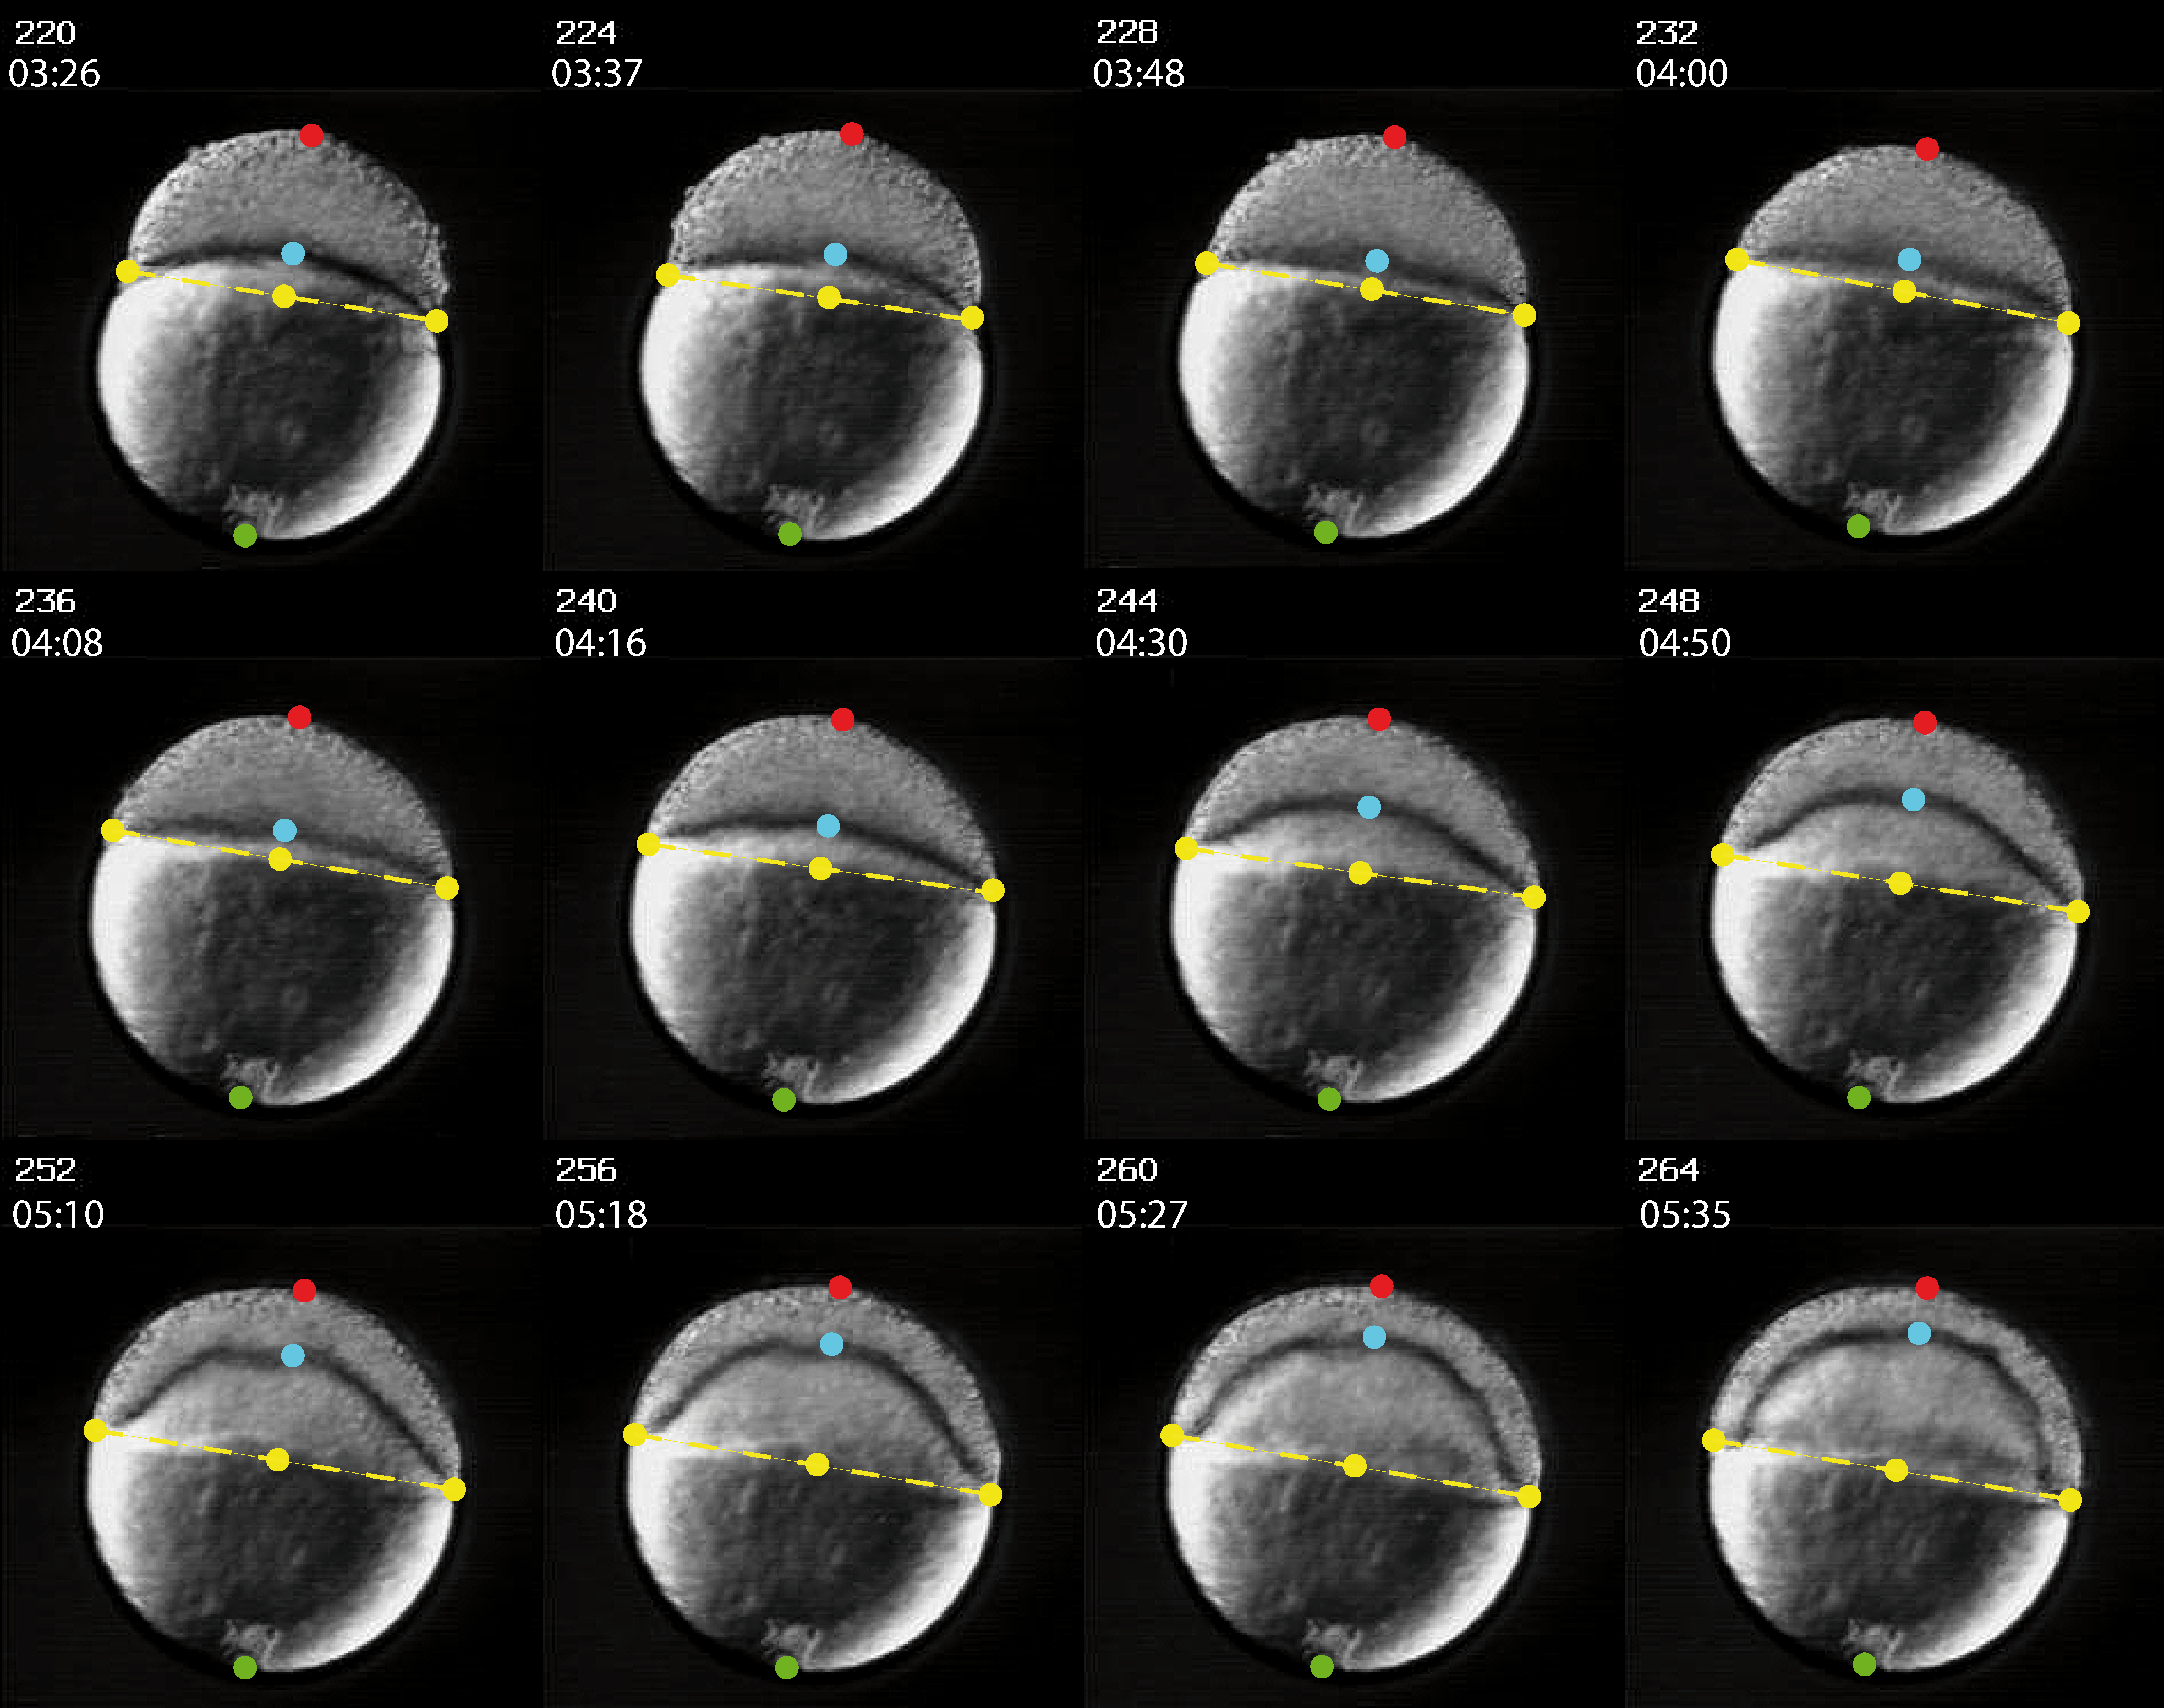
\includegraphics[width=0.8\textwidth]{../../images/Cases_Studies/Case_4_intercalation/kane_dev/fusion.png}
\end{center}
\caption{\textbf{Macroscopic landmarks of the epibolic deformation.} The snapshots of the zebrafish development from the oblong stage to 50 percent epiboly are extracted from the movie \href{http://public.iscpif.fr/~delile/morphogenesis/manuscript/pragma/figure.html?name=Zebra_Zebrafish_Development_kane}{.S.5} by Karlstrom and Kane \cite{Karlstrom:1996wo}. Colored dots has been manually added by visual estimating the following morphological macroscopic measures: the red dot gives the position of the animal region of the embryo, the green dot gives the position of the vegetal region of the embryo, the blue dot gives the animal region of the yolk cell, the two lateral yellow dots gives the position of the margin and the central yellow dot is the projection of margin dots on the animal-vegetal axis. The time value displayed below the image id is the time in hour post fertilization given by \cite{Karlstrom:1996wo}. This times does not scale linearly with the image ids and have been renormalized.}
\label{kane_dev_fusion}
\end{figure}
\begin{figure}
\begin{center}
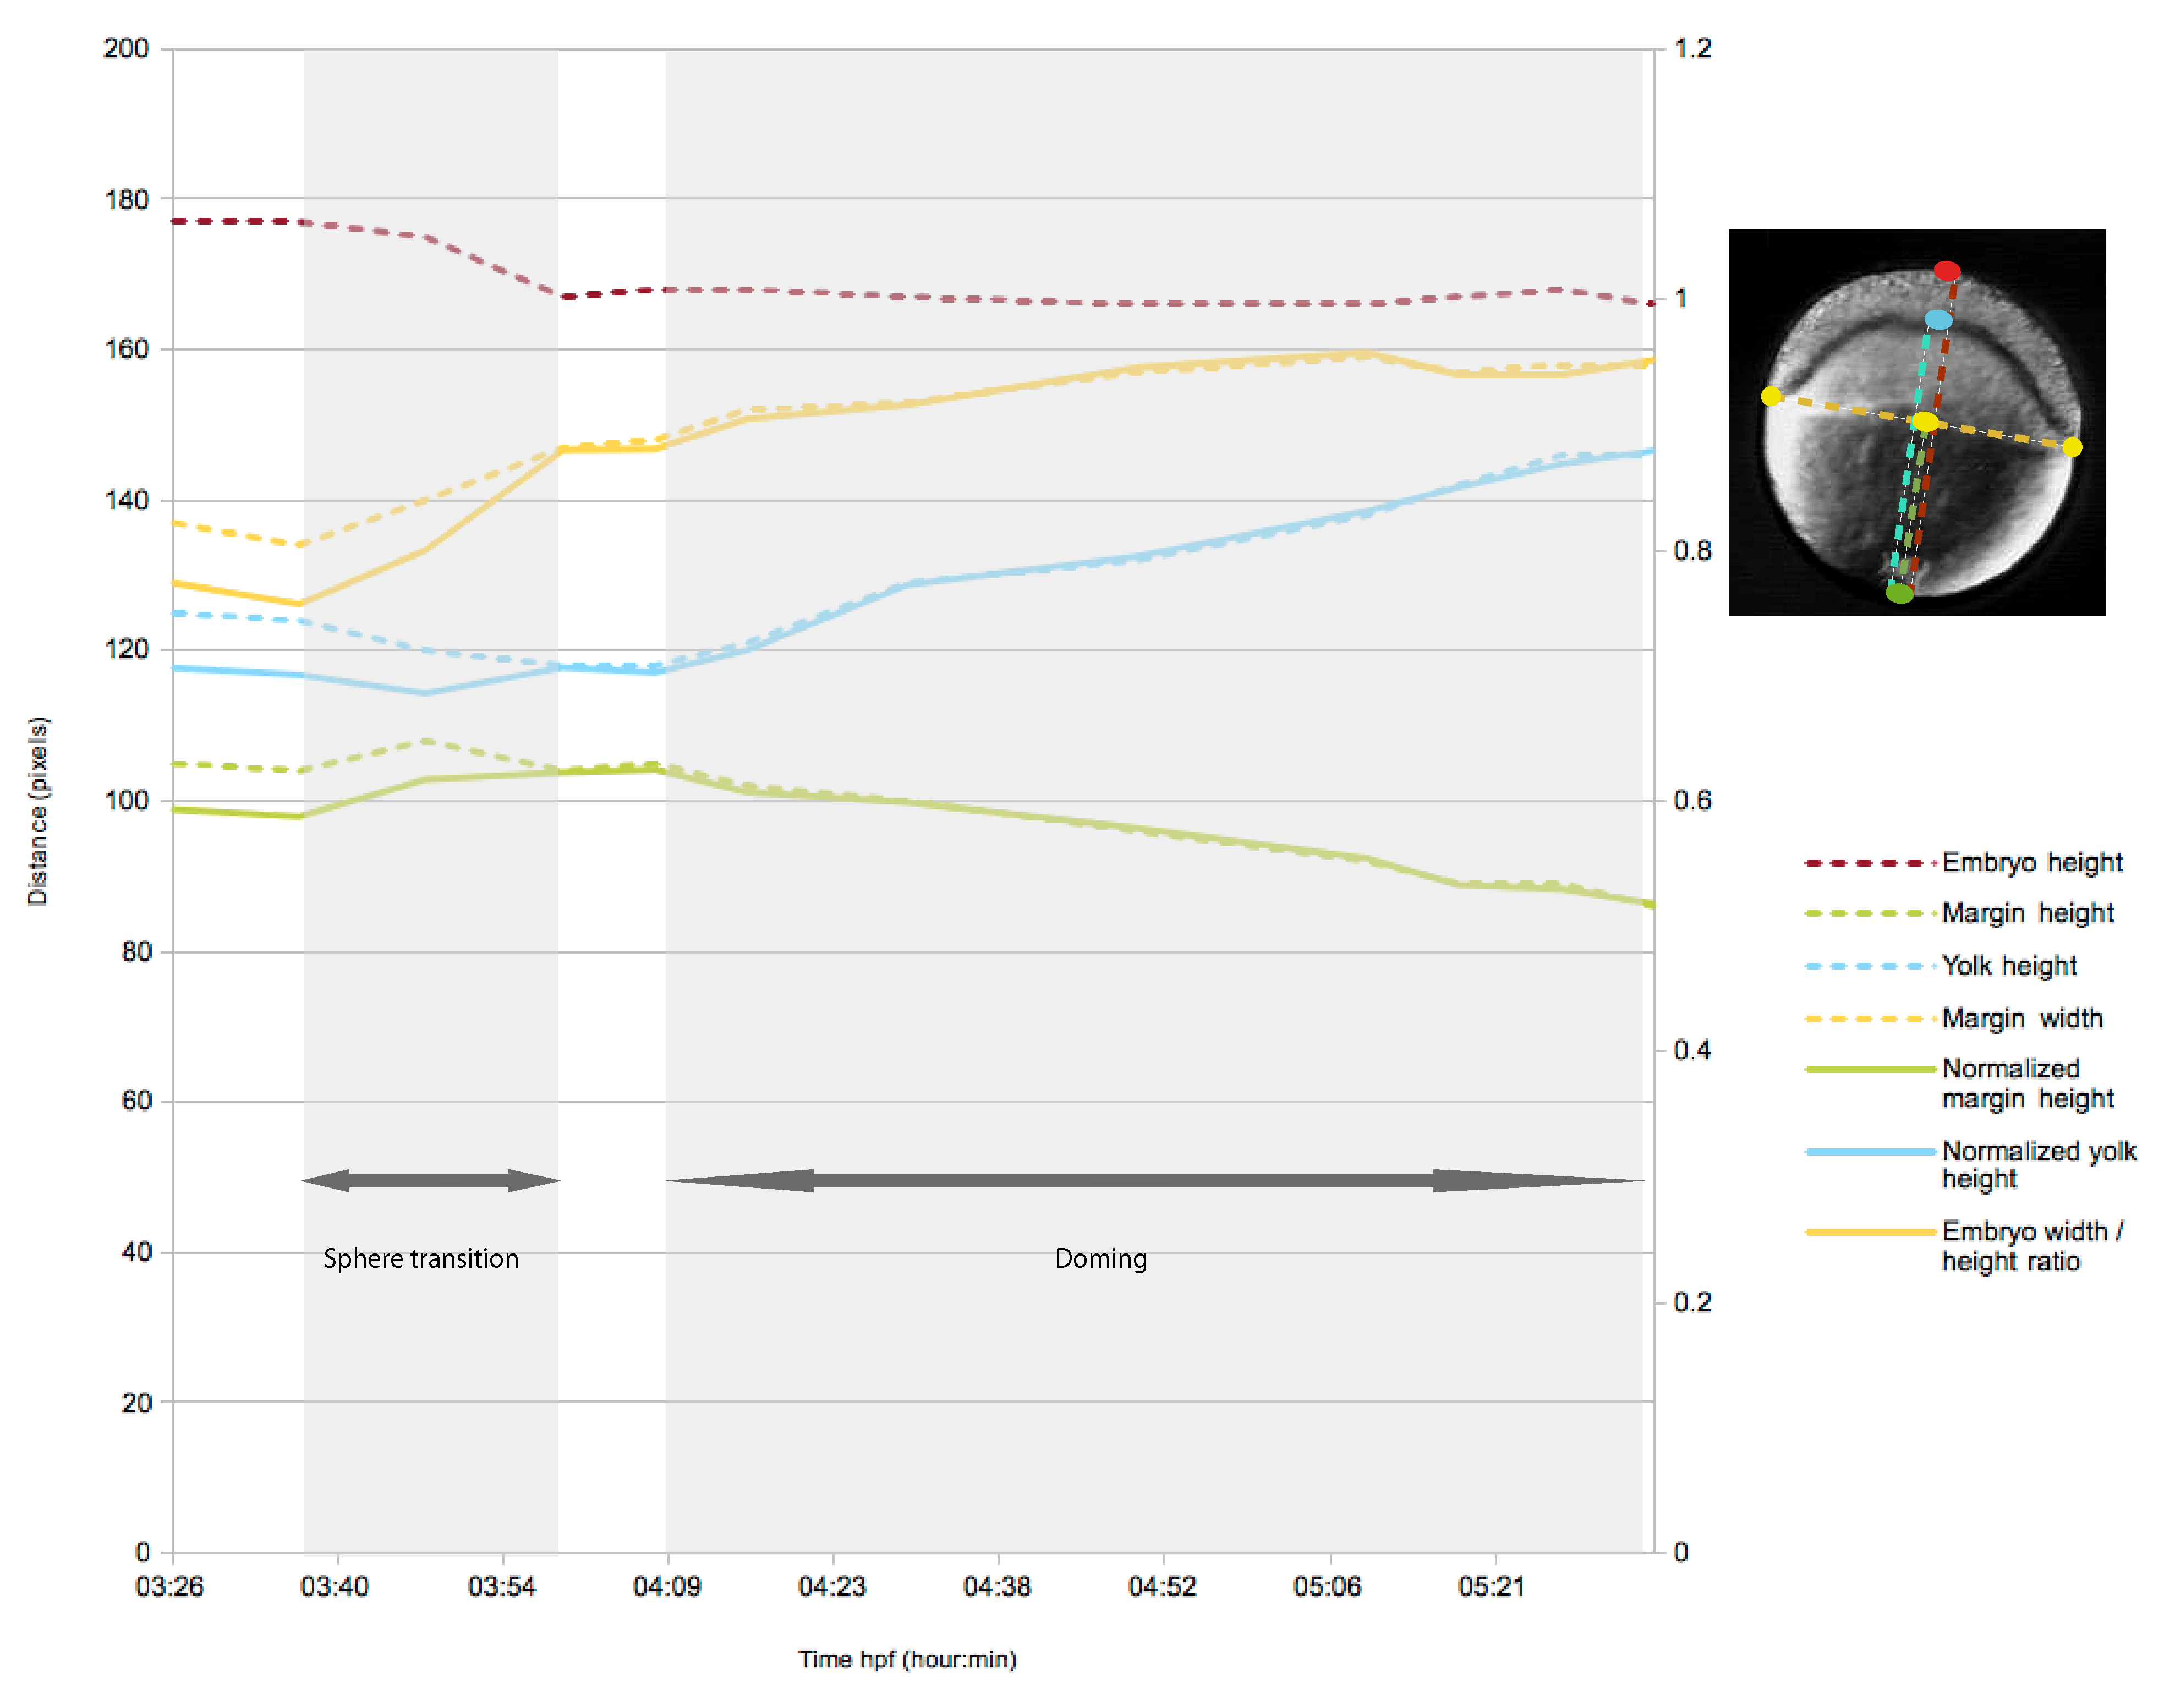
\includegraphics[width=0.8\textwidth]{../../images/Cases_Studies/Case_4_intercalation/kane_dev/fusion_plot.png}
\end{center}
\caption{\textbf{Macroscopic measures of the epibolic deformation.} The distances defined by the macroscopic landmarks displayed in Fig. \ref{kane_dev_fusion} are shown. The red line is the plot of the distance between the animal region of the embryo and the vegetal region of the yolk (embryo height). The green line is the plot of the distance between the projection of the margin on the animal-vegetal axis and the vegetal region of the yolk (margin height). The blue line is distance between the animal region of the yolk and the vegetal region of the yolk (yolk height). The yellow line is the lateral distance between lateral margin position. The dashed lines give the absolute distance between landmarks in pixels and scale on the left ordinate axis. The continuous lines give the normalized distance and scale on the right ordinate axis. The normalization is obtained by dividing each value by the current yolk height (i.e. dashed red line). The abscissa gives the time in hour post fertilization.}
\label{kane_dev_fusion_plot}
\end{figure}    figure   

  il faut normaliser pour comparer les embryons, mais la normalization fait perdre de l'information.  example: diviser par la hauteur AV de l'embryon et on perd son aplatissement 

  -> il faut plusieurs mesures    Observations kane macro measure -> normalized margin height monte un peu durant sphere transition (mais pas en absolue)  Reconstruction simulated embryos:  expliquer max yolk , min yolk , max evl, et surtout margin. contrairement au live qui est 2D, dans l'embryon simulé 3D.  Exploration selon source evl ou yolk  on espere voir une difference sur le ratio margin / height  aplatissement plus intéressant si from yolk    Resultats:   dans la simu, l'applatissement et le doming sont simultanés, et la marge est un peu plus tard dans le live, l'applatissement commence avant le doming (yolk + marge simultanée)  -> il faudrait que la marge subisse plus l'etalement         Résultats:  .compromis force/stochasticité,      Discussion:  measure microscopiques permetrons peut etre de characteriser l'intensité de la force de protrusion, qui est un parametre discutable: quel est sont range réel? les cellules n'ont pas une force de protrusion illimité.  correlation entre mesures micro et mesures macro    

\subsubsection{Hypotheses and Model }

\subsubsection{Simulation, Parameter Space and Validation }

  We observe the evolution of the cell position at the onset of epiboly. 
\begin{figure}
\begin{center}
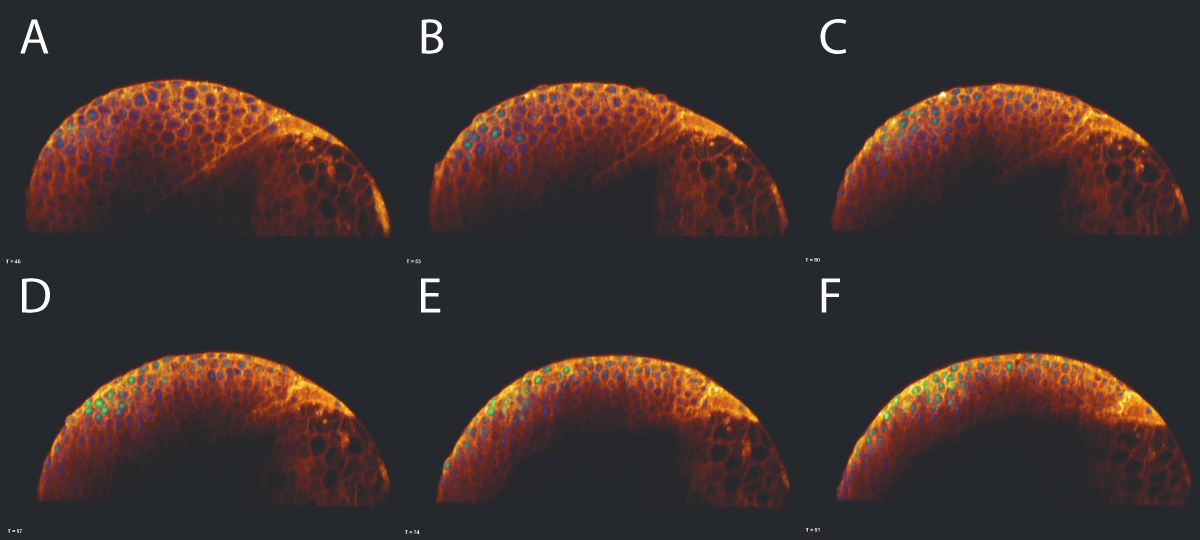
\includegraphics[width=0.9\textwidth]{../../images/Cases_Studies/Case_4_intercalation/071222bF_horizontal.png}
\end{center}
\caption{071222bF}
\label{Case_4_intercalation_071222bF_horizontal}
\end{figure}
\begin{figure}
\begin{center}
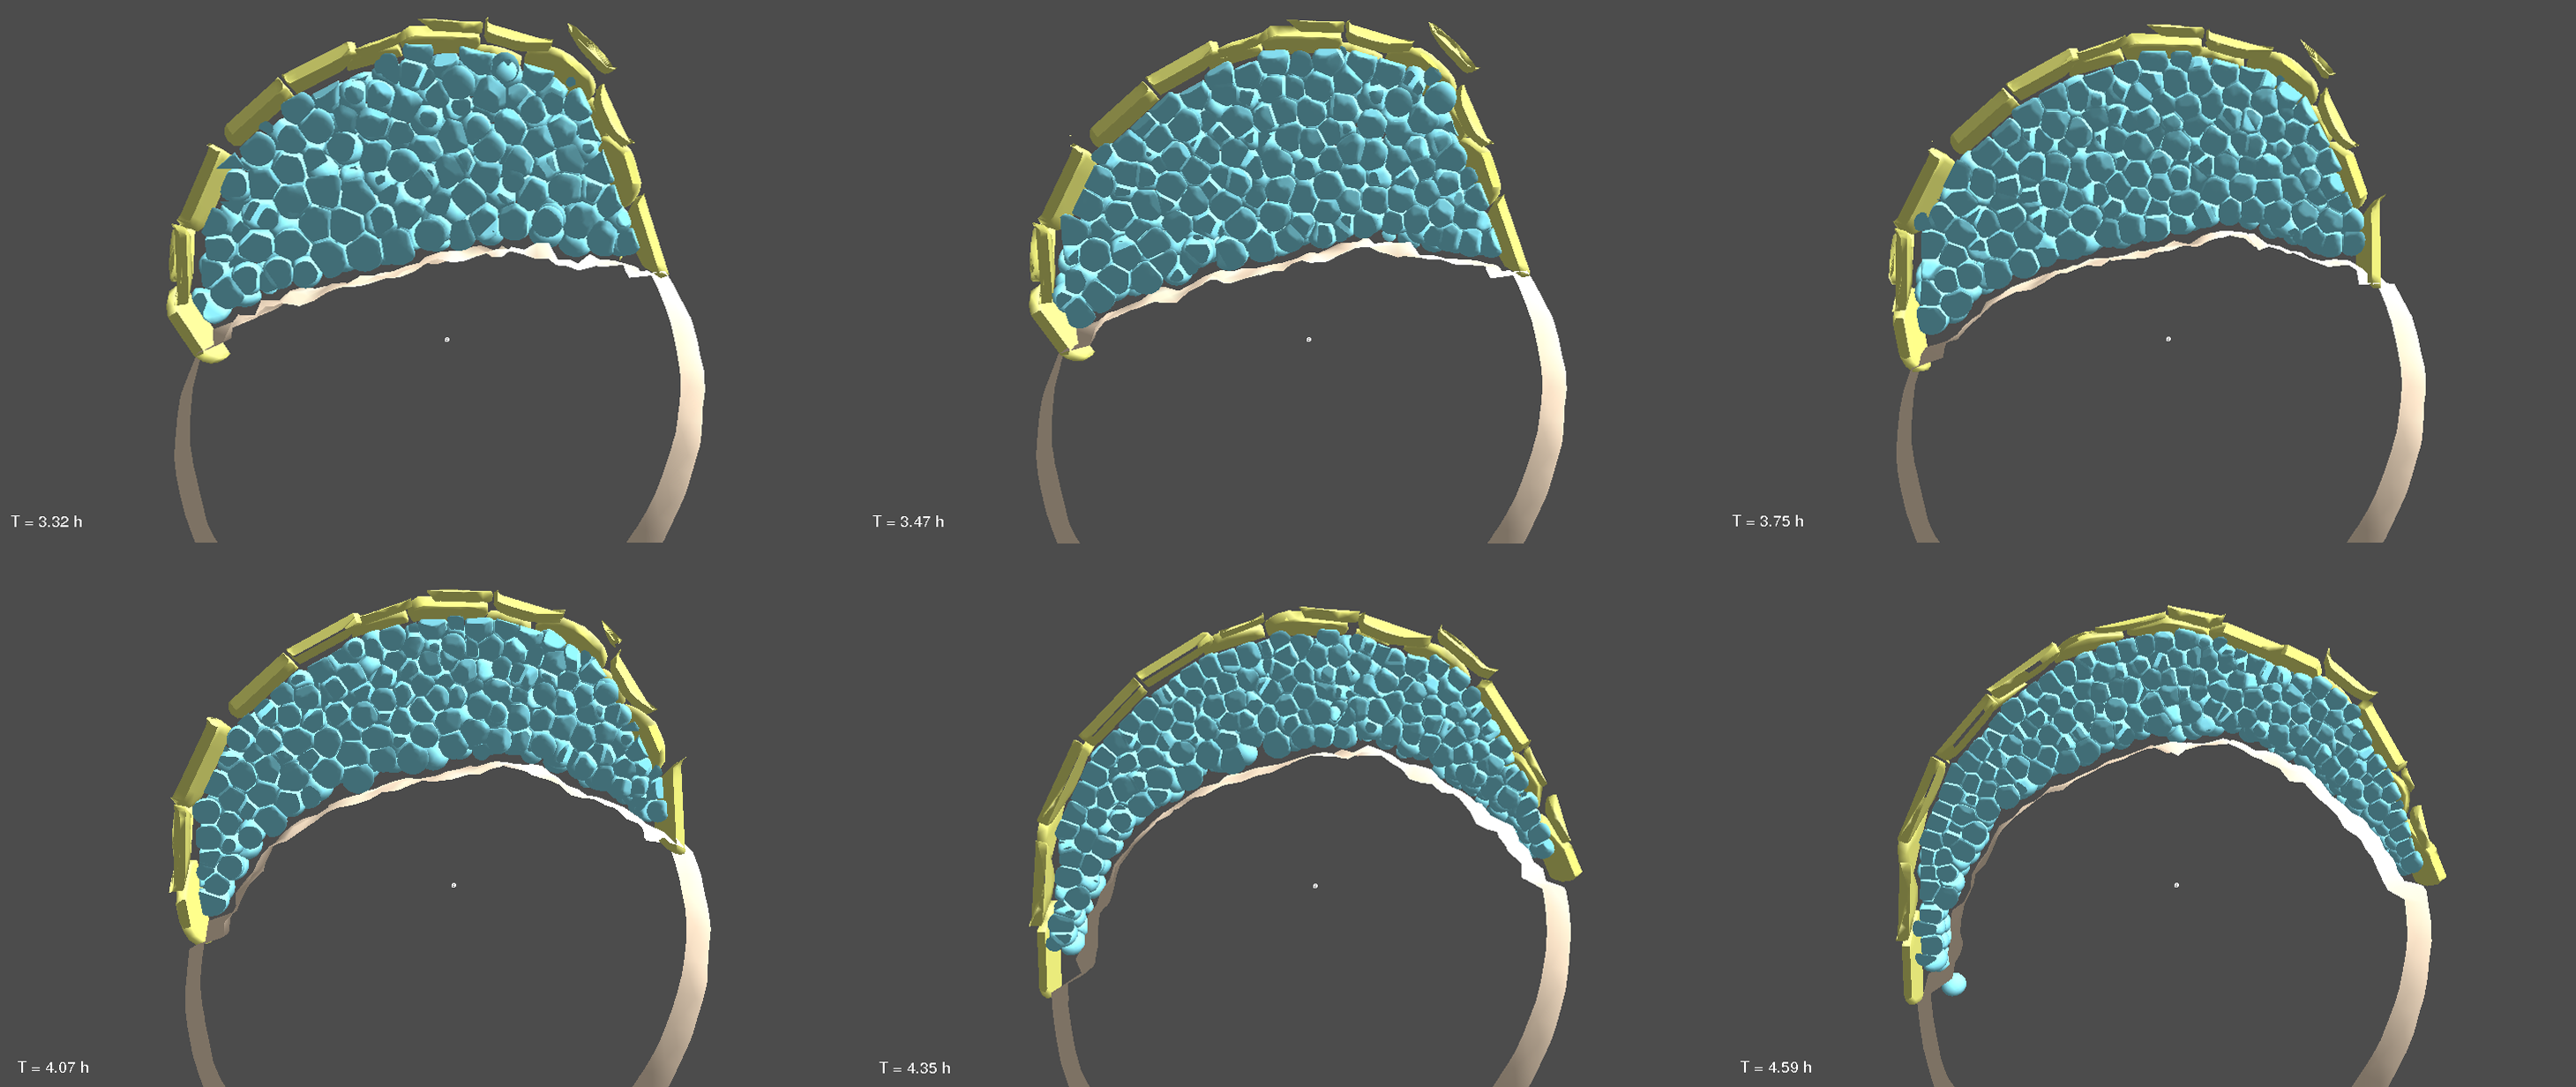
\includegraphics[width=0.9\textwidth]{../../images/Cases_Studies/Case_4_intercalation/simulation/general/simulation_general.png}
\end{center}
\caption{}
\label{simulation_general}
\end{figure}

\paragraph{Reconstruction}

  Let $T_s$ be the starting time step of the measure. At $T_s$, each cell receives a label (total $N_{label}$). As time advances and cells divide, daughter cells will inherit the label of their mother.  

  We measure at each time step which label has a neighboring contact with another label. This measure is represented by a square matrix $C(t)$ of size $N_{label} \times N_{label} $. An element $c_{i,j}(t)$ of the matrix has a value of 1 if at least a cell having a label i is in contact with at least a cell having a label j at the current time step. Otherwise, $c_{i,j}(t)$ is 0. 

  A time integration of the matrix indicates which cell lineage is. 
\begin{figure}
\begin{center}
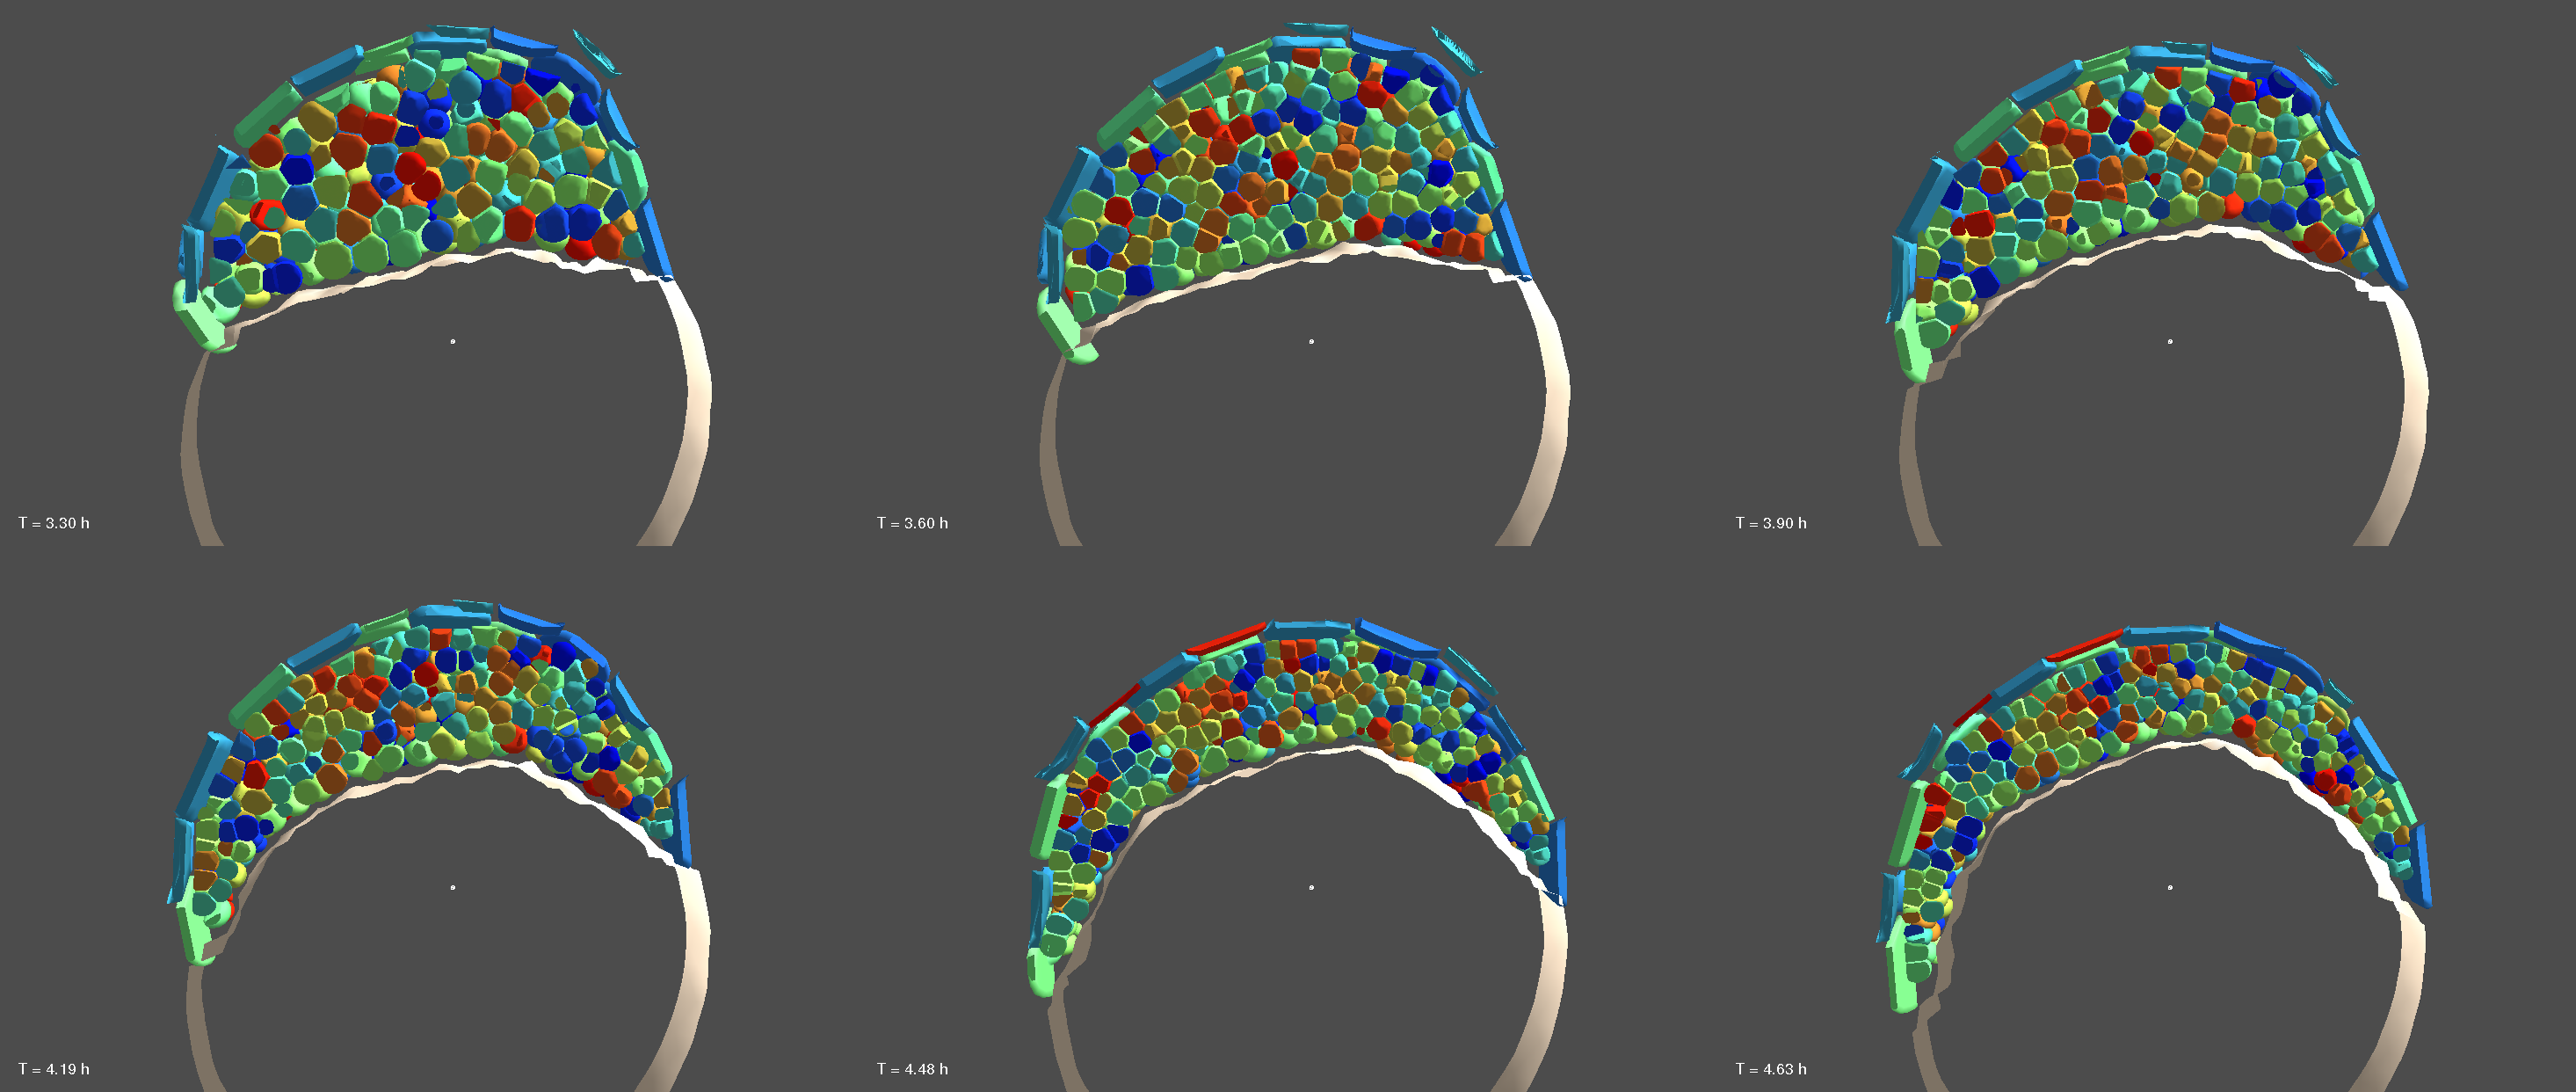
\includegraphics[width=0.9\textwidth]{../../images/Cases_Studies/Case_4_intercalation/simulation/clonal/simulation_clonal.png}
\end{center}
\caption{Cell lineage with label.}
\label{simulation_clonal}
\end{figure}
\begin{figure}
\begin{center}
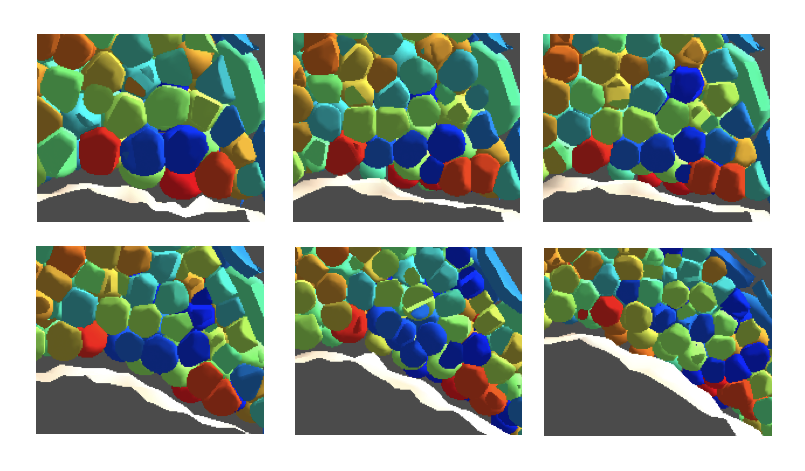
\includegraphics[width=0.7\textwidth]{../../images/Cases_Studies/Case_4_intercalation/simulation/mitosis_clonal/simulation_mitosis_clonal.png}
\end{center}
\caption{Zoom on mitoses to highlight/show label inheritance.}
\label{simulation_mitosis_clonal}
\end{figure}



\subsubsection{Discussion  }

\subsection{Gastrulation  }             epiboly pre 50%:   orientation radiale est plutot donné par yolk et non par l'evl   argument 1: espace entre blasto et evl assez tot, voir film 071222bF 3sec environ           

   Epiboly post internalization  

   hypothese: hypoblast migrates on the epiblast, and it favors the epiboly movement. See example of MZOEP mutant which is slower (figure below).  
\begin{figure}
\begin{center}
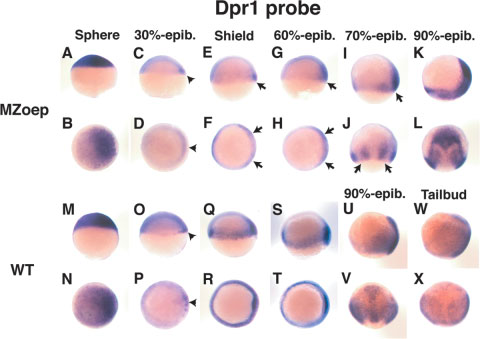
\includegraphics[width=0.8\textwidth]{../../images/Cases_Studies/Case_7_Convergence_extension/waxman_2005.png}
\end{center}
\caption{from Waxman, J.S., 2005. Regulation of the early expression patterns of the zebrafish Dishevelled-interacting proteins Dapper1 and Dapper2. Developmental dynamics : an official publication of the American Association of Anatomists, 233(1), pp.194–200. \cite{Waxman:2005fe}. Epiboly is slower - "Note that, because later epiboly (epib.) movements are delayed in MZoep embryos, dpr1 expression in MZoep embryos at $70\%$ and $90\%$ epiboly is compared with wild-type embryos at $90\%$ epiboly and tail bud stages, respectively."}
\label{Case_Epi_Convergence_extension_waxman_2005}
\end{figure}

\subsubsection{Internalization  }

\subsubsection{Margin contraction  }

\subsubsection{Convergence-Extension  }

\textbf{Hypotheses}

  Initial state of the case study: 
\begin{itemize}
	\item cell position: internalized embryo 60% epiboly
	\item polarization field: (verifier sur ancien fichier)
\end{itemize}

\textbf{Questions}

  Background (bio): 

  The formation of the antero-posterior axis of the embryo is associated with an elongation of the tissue. 

  Various cellular mechanisms may be responsible for an elongation (growth along a preferential axis): 
\begin{itemize}
	\item cell deformation along the APaxis: C. elegans, Phallusia (ascidians ?)
	\item active cell rearrangement: chord Pallusia, Drosophila
	\item oriented cell division, amplified with cell growth: XXXX ??
\end{itemize}

  During the zebrafish gastrulation, this episode is called Convergence-Extension (CE) (see Review chapitre 6 XXX). 

\paragraph{Q1. Influence of the division orientation axis on the convergence}

  -> Is it possible to have a convergence-extension behavior if the division orientation axes are random ? we can test it 

  -> Does it help to have oriented division axes along the XXXXX ? we can test it 

  We postulate that cell are re-oriented after division because of the external protrusive activity around them. On peut le montrer en mettant des divisions d'axes random et en plotant la reorientation dû aux actions mechaniques locales (protrusions des voisines.) 

  Biblio: 

\textit{In vivo} confocal imaging shows that mitotic divisions in the dorsal region of the zebrafish gastrulation are preferentially oriented along the animal vegetal axis and this orientation is a driving force of axis elongation \cite{Gong:2004bw}

   "Xdd1 disrupts convergence and extension of the dorsal tissue (Fig. 4b)11,13. It is thus possible that the disruption of oriented division observed in Xdd1-overexpressing embryos was due to compromised morphogenesis of the tissue. To address this, we generated mosaic clones of Xdd1-expressing cells in a wild-type background by injecting a single cleavage-stage blastomere. Such embryos undergo normal morphogenesis, and are indistinguishable from unmanipulated controls morphologically (data not shown). Subsequent analysis shows that these mosaic Xdd1-expressing cells have randomized division orientation, with angular distribution similar to that of embryos overexpressing Xdd1 ubiquitously (Fig. 3e, f; see Supplementary Information for details). Thus, Dsh has a cell-autonomous function and exerts its effect on division orientation directly." ... "Our experiments on the zebrafish dorsal epiblast show both a matching of division orientation and axis elongation normally, and a disruption of oriented cell division and axis elongation after inhibition of PCP signalling. We assessed the contribution of oriented cell division to axis elongation." (Gong, Y., Mo, C. \& Fraser, S.E., 2004. Planar cell polarity signalling controls cell division orientation during zebrafish gastrulation. Nature, 430(7000), pp.689–693. \cite{Gong:2004bw}) -> still a double, another mechanism, like protrusion, could also be involved. leaving this cell division orientation bias as a side effect. It would be really interesting to check in my simulation if, even with random axis, cell are re-oriented by protrusive mechanism (deactivate protrusion for the dividing cell and check if there is many differences).  

   see Segalen, M. \& Bellaã che, Y., 2009. Cell division orientation and planar cell polarity pathways. Seminars in Cell and Developmental Biology, pp.1–6. \cite{Segalen:2009fg}

  Measures, see papier Manu 
\begin{itemize}
	\item local velocity vector
	\item mitotic dipole as a function of time, evolution of the distance -> daughter cells which 
\end{itemize}    zoep: pas de plaque prechordale, pas d'endoderme -> mesoderme se debrouille    

\paragraph{Q2. Effect of the hypoblast CE on the epiblast CE.}
\begin{figure}
\begin{center}
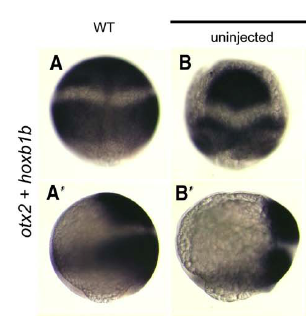
\includegraphics[width=0.5\textwidth]{../../images/Cases_Studies/Case_7_Convergence_extension/jia_2009.png}
\end{center}
\caption{WT and MZoep from Jia, S. et al., 2009. Smad2/3 activities are required for induction and patterning of the neuroectoderm in zebrafish. Developmental Biology, 333(2), pp.273–284. \cite{Jia:2009ez}. The extension is less decreased and the mass of converged cell is concentrated in the posterior region.}
\label{Case_7_Convergence_extension/jia_2009}
\end{figure}
\begin{figure}
\begin{center}
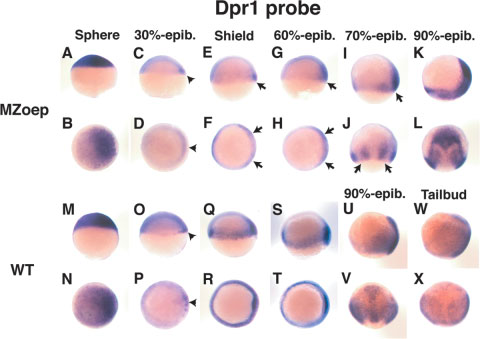
\includegraphics[width=0.8\textwidth]{../../images/Cases_Studies/Case_7_Convergence_extension/waxman_2005.png}
\end{center}
\caption{from Waxman, J.S., 2005. Regulation of the early expression patterns of the zebrafish Dishevelled-interacting proteins Dapper1 and Dapper2. Developmental dynamics : an official publication of the American Association of Anatomists, 233(1), pp.194–200. \cite{Waxman:2005fe}. Epiboly is slower - "Note that, because later epiboly (epib.) movements are delayed in MZoep embryos, dpr1 expression in MZoep embryos at $70\%$ and $90\%$ epiboly is compared with wild-type embryos at $90\%$ epiboly and tail bud stages, respectively."}
\label{Case_7_Convergence_extension/waxman_2005}
\end{figure}

  MZoep mutant does not internalize properly and lacks mesendoderm and structures (notochord, prechordal plate, paraxial/lateral mesendoderm).   

  MZoep is a mutant of the Nodal-signaling pathways and the Nodal-dependent gene (XXXX goosecoid,...) are not expressed. see Jia, S. et al., 2009. Smad2/3 activities are required for induction and patterning of the neuroectoderm in zebrafish. Developmental Biology, 333(2), pp.273–284. \cite{Jia:2009ez}

  However, its epiblast still performs a CE.    Dorsalizing genes are still expressed (XXXXX)   Its phenotype shows that the cell mass is present at the dorsal side but in a more ventral latitude (show image). 

  We postulate that the epiblast CE is unaffected by the lack of hypoblast mechanically. Its different phenotype is due to a change in the polarization field in the tissue whose difference correlates with lack of polarization source in the region of the prechorlale plate. 

  -> exemple de modelisation qui suggere une expérience: reorienter le champ en injectant qqchose au niveau de la plaque prechordale 

  Measures: 
\begin{itemize}
	\item point singulier voir Thierry et David Pastor. demander à Thierry...
	\item evolution of the convergence half ring from Carmany-Rampey, A. & Schier, A.F., 2001. Single-cell internalization during zebrafish gastrulation. Current biology : CB, 11(16), pp.1261–1265. 
	\item clonal cells alignment. see clonal modes from Petit, A.-C., Legué, E. & Nicolas, J.F., 2005. Methods in clonal analysis and applications. Reproduction Nutrition Development, 45(3), pp.321–339. \cite{Petit:2005dp}
\end{itemize}
\begin{figure}
\begin{center}
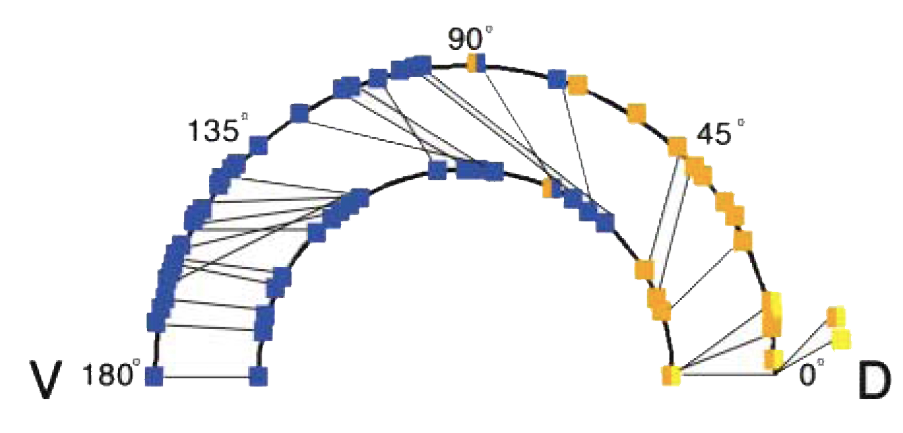
\includegraphics[width=0.6\textwidth]{../../images/Cases_Studies/Case_7_Convergence_extension/carmany_rampey_2001.png}
\end{center}
\caption{from Carmany-Rampey, A. & Schier, A.F., 2001. Single-cell internalization during zebrafish gastrulation. Current biology : CB, 11(16), pp.1261–1265. \cite{CarmanyRampey:2001uy}}
\label{Case_7_Convergence_extension_carmany_rampey_2001}
\end{figure}

\paragraph{Q3. Contribution of the CE to the epiboly.}

\subparagraph{Background}







\subsubsection{Hypotheses and Model  }

\subsubsection{Simulation, Parameter Space and Validation }

\subsubsection{Discussion  }
